%**************************************%
%*    Generated from PreTeXt source   *%
%*    on 2020-01-19T09:59:57-06:00    *%
%*                                    *%
%*      https://pretextbook.org       *%
%*                                    *%
%**************************************%
\documentclass[oneside,10pt,]{book}
%% Custom Preamble Entries, early (use latex.preamble.early)
%% Default LaTeX packages
%%   1.  always employed (or nearly so) for some purpose, or
%%   2.  a stylewriter may assume their presence
\usepackage{geometry}
%% Some aspects of the preamble are conditional,
%% the LaTeX engine is one such determinant
\usepackage{ifthen}
%% etoolbox has a variety of modern conveniences
\usepackage{etoolbox}
\usepackage{ifxetex,ifluatex}
%% Raster graphics inclusion
\usepackage{graphicx}
%% Color support, xcolor package
%% Always loaded, for: add/delete text, author tools
%% Here, since tcolorbox loads tikz, and tikz loads xcolor
\PassOptionsToPackage{usenames,dvipsnames,svgnames,table}{xcolor}
\usepackage{xcolor}
%% begin: defined colors, via xcolor package, for styling
%% end: defined colors, via xcolor package, for styling
%% Colored boxes, and much more, though mostly styling
%% skins library provides "enhanced" skin, employing tikzpicture
%% boxes may be configured as "breakable" or "unbreakable"
%% "raster" controls grids of boxes, aka side-by-side
\usepackage{tcolorbox}
\tcbuselibrary{skins}
\tcbuselibrary{breakable}
\tcbuselibrary{raster}
%% We load some "stock" tcolorbox styles that we use a lot
%% Placement here is provisional, there will be some color work also
%% First, black on white, no border, transparent, but no assumption about titles
\tcbset{ bwminimalstyle/.style={size=minimal, boxrule=-0.3pt, frame empty,
colback=white, colbacktitle=white, coltitle=black, opacityfill=0.0} }
%% Second, bold title, run-in to text/paragraph/heading
%% Space afterwards will be controlled by environment,
%% dependent of constructions of the tcb title
\tcbset{ runintitlestyle/.style={fonttitle=\normalfont\bfseries, attach title to upper} }
%% Spacing prior to each exercise, anywhere
\tcbset{ exercisespacingstyle/.style={before skip={1.5ex plus 0.5ex}} }
%% Spacing prior to each block
\tcbset{ blockspacingstyle/.style={before skip={2.0ex plus 0.5ex}} }
%% xparse allows the construction of more robust commands,
%% this is a necessity for isolating styling and behavior
%% The tcolorbox library of the same name loads the base library
\tcbuselibrary{xparse}
%% Hyperref should be here, but likes to be loaded late
%%
%% Inline math delimiters, \(, \), need to be robust
%% 2016-01-31:  latexrelease.sty  supersedes  fixltx2e.sty
%% If  latexrelease.sty  exists, bugfix is in kernel
%% If not, bugfix is in  fixltx2e.sty
%% See:  https://tug.org/TUGboat/tb36-3/tb114ltnews22.pdf
%% and read "Fewer fragile commands" in distribution's  latexchanges.pdf
\IfFileExists{latexrelease.sty}{}{\usepackage{fixltx2e}}
%% shorter subnumbers in some side-by-side require manipulations
\usepackage{xstring}
%% Text height identically 9 inches, text width varies on point size
%% See Bringhurst 2.1.1 on measure for recommendations
%% 75 characters per line (count spaces, punctuation) is target
%% which is the upper limit of Bringhurst's recommendations
\geometry{letterpaper,total={340pt,9.0in}}
%% Custom Page Layout Adjustments (use latex.geometry)
%% This LaTeX file may be compiled with pdflatex, xelatex, or lualatex executables
%% LuaTeX is not explicitly supported, but we do accept additions from knowledgeable users
%% The conditional below provides  pdflatex  specific configuration last
%% The following provides engine-specific capabilities
%% Generally, xelatex is necessary for non-Western fonts
\ifthenelse{\boolean{xetex} \or \boolean{luatex}}{%
%% begin: xelatex and lualatex-specific configuration
\ifxetex\usepackage{xltxtra}\fi
%% realscripts is the only part of xltxtra relevant to lualatex 
\ifluatex\usepackage{realscripts}\fi
%% fontspec package provides extensive control of system fonts,
%% meaning *.otf (OpenType), and apparently *.ttf (TrueType)
%% that live *outside* your TeX/MF tree, and are controlled by your *system*
%% (it is possible that a TeX distribution will place fonts in a system location)
\usepackage{fontspec}
%% We use Latin Modern (lmodern) as the default font
%% So we check that it is available as a system font
\IfFontExistsTF{Latin Modern Roman}{}{\GenericError{}{The font "Latin Modern Roman" requested by PreTeXt output is not available as a system font}{Consult the PreTeXt Guide for help with LaTeX fonts.}{}}
%% We then define various font family commands using a vanilla version,
%% with the intention of letting a style override these choices
%% \setmainfont can be re-issued, and \renewfontfamily can redefine others
\setmainfont{Latin Modern Roman}[SmallCapsFont={Latin Modern Roman Caps}, SlantedFont={Latin Modern Roman Slanted}]
\newfontfamily{\divisionfont}{Latin Modern Roman}
\newfontfamily{\contentsfont}{Latin Modern Roman}
\newfontfamily{\pagefont}{Latin Modern Roman}[SlantedFont={Latin Modern Roman Slanted}]
\newfontfamily{\tabularfont}{Latin Modern Roman}[SmallCapsFont={Latin Modern Roman Caps}]
%% begin: font information supplied by "font-xelatex-style" template
%% end: font information supplied by "font-xelatex-style" template
%% 
%% Extensive support for other languages
\usepackage{polyglossia}
%% Set main/default language based on pretext/@xml:lang value
%% document language code is "en-US", US English
%% usmax variant has extra hypenation
\setmainlanguage[variant=usmax]{english}
%% Enable secondary languages based on discovery of @xml:lang values
%% Enable fonts/scripts based on discovery of @xml:lang values
%% Western languages should be ably covered by Latin Modern Roman
%% end: xelatex and lualatex-specific configuration
}{%
%% begin: pdflatex-specific configuration
\usepackage[utf8]{inputenc}
%% PreTeXt will create a UTF-8 encoded file
%% begin: font setup and configuration for use with pdflatex
%% Portions of a document, are, or may, be affected by font-changing commands
%% These are more robust when using  xelatex  but may be employed with  pdflatex
%% The following definitons are meant to be re-defined in a style with \renewcommand
\newcommand{\divisionfont}{\relax}
\newcommand{\contentsfont}{\relax}
\newcommand{\pagefont}{\relax}
\newcommand{\tabularfont}{\relax}
%% begin: font information supplied by "font-pdflatex-style" template
\usepackage{lmodern}
\usepackage[T1]{fontenc}
%% begin: font information supplied by "font-pdflatex-style" template
%% end: font setup and configuration for use with pdflatex
%% end: pdflatex-specific configuration
}
%% Symbols, align environment, bracket-matrix
\usepackage{amsmath}
\usepackage{amssymb}
%% allow page breaks within display mathematics anywhere
%% level 4 is maximally permissive
%% this is exactly the opposite of AMSmath package philosophy
%% there are per-display, and per-equation options to control this
%% split, aligned, gathered, and alignedat are not affected
\allowdisplaybreaks[4]
%% allow more columns to a matrix
%% can make this even bigger by overriding with  latex.preamble.late  processing option
\setcounter{MaxMatrixCols}{30}
%%
%%
%% Division Titles, and Page Headers/Footers
%% titlesec package, loading "titleps" package cooperatively
%% See code comments about the necessity and purpose of "explicit" option.
%% The "newparttoc" option causes a consistent entry for parts in the ToC 
%% file, but it is only effective if there is a \titleformat for \part.
%% "pagestyles" loads the  titleps  package cooperatively.
\usepackage[explicit, newparttoc, pagestyles]{titlesec}
%% The companion titletoc package for the ToC.
\usepackage{titletoc}
%% Fixes a bug with transition from chapters to appendices in a "book"
%% See generating XSL code for more details about necessity
\newtitlemark{\chaptertitlename}
%% begin: customizations of page styles via the modal "titleps-style" template
%% Designed to use commands from the LaTeX "titleps" package
%% Plain pages should have the same font for page numbers
\renewpagestyle{plain}{%
\setfoot{}{\pagefont\thepage}{}%
}%
%% Single pages as in default LaTeX
\renewpagestyle{headings}{%
\sethead{\pagefont\slshape\MakeUppercase{\ifthechapter{\chaptertitlename\space\thechapter.\space}{}\chaptertitle}}{}{\pagefont\thepage}%
}%
\pagestyle{headings}
%% end: customizations of page styles via the modal "titleps-style" template
%%
%% Create globally-available macros to be provided for style writers
%% These are redefined for each occurence of each division
\newcommand{\divisionnameptx}{\relax}%
\newcommand{\titleptx}{\relax}%
\newcommand{\subtitleptx}{\relax}%
\newcommand{\shortitleptx}{\relax}%
\newcommand{\authorsptx}{\relax}%
\newcommand{\epigraphptx}{\relax}%
%% Create environments for possible occurences of each division
%% Environment for a PTX "acknowledgement" at the level of a LaTeX "chapter"
\NewDocumentEnvironment{acknowledgement}{mmmmmm}
{%
\renewcommand{\divisionnameptx}{Acknowledgements}%
\renewcommand{\titleptx}{#1}%
\renewcommand{\subtitleptx}{#2}%
\renewcommand{\shortitleptx}{#3}%
\renewcommand{\authorsptx}{#4}%
\renewcommand{\epigraphptx}{#5}%
\chapter*{#1}%
\addcontentsline{toc}{chapter}{#3}
\label{#6}%
}{}%
%% Environment for a PTX "preface" at the level of a LaTeX "chapter"
\NewDocumentEnvironment{preface}{mmmmmm}
{%
\renewcommand{\divisionnameptx}{Preface}%
\renewcommand{\titleptx}{#1}%
\renewcommand{\subtitleptx}{#2}%
\renewcommand{\shortitleptx}{#3}%
\renewcommand{\authorsptx}{#4}%
\renewcommand{\epigraphptx}{#5}%
\chapter*{#1}%
\addcontentsline{toc}{chapter}{#3}
\label{#6}%
}{}%
%% Environment for a PTX "chapter" at the level of a LaTeX "chapter"
\NewDocumentEnvironment{chapterptx}{mmmmmm}
{%
\renewcommand{\divisionnameptx}{Chapter}%
\renewcommand{\titleptx}{#1}%
\renewcommand{\subtitleptx}{#2}%
\renewcommand{\shortitleptx}{#3}%
\renewcommand{\authorsptx}{#4}%
\renewcommand{\epigraphptx}{#5}%
\chapter[{#3}]{#1}%
\label{#6}%
}{}%
%% Environment for a PTX "section" at the level of a LaTeX "section"
\NewDocumentEnvironment{sectionptx}{mmmmmm}
{%
\renewcommand{\divisionnameptx}{Section}%
\renewcommand{\titleptx}{#1}%
\renewcommand{\subtitleptx}{#2}%
\renewcommand{\shortitleptx}{#3}%
\renewcommand{\authorsptx}{#4}%
\renewcommand{\epigraphptx}{#5}%
\section[{#3}]{#1}%
\label{#6}%
}{}%
%% Environment for a PTX "exercises" at the level of a LaTeX "subsection"
\NewDocumentEnvironment{exercises-subsection}{mmmmmm}
{%
\renewcommand{\divisionnameptx}{Exercises}%
\renewcommand{\titleptx}{#1}%
\renewcommand{\subtitleptx}{#2}%
\renewcommand{\shortitleptx}{#3}%
\renewcommand{\authorsptx}{#4}%
\renewcommand{\epigraphptx}{#5}%
\subsection[{#3}]{#1}%
\label{#6}%
}{}%
%% Environment for a PTX "exercises" at the level of a LaTeX "subsection"
\NewDocumentEnvironment{exercises-subsection-numberless}{mmmmmm}
{%
\renewcommand{\divisionnameptx}{Exercises}%
\renewcommand{\titleptx}{#1}%
\renewcommand{\subtitleptx}{#2}%
\renewcommand{\shortitleptx}{#3}%
\renewcommand{\authorsptx}{#4}%
\renewcommand{\epigraphptx}{#5}%
\subsection*{#1}%
\addcontentsline{toc}{subsection}{#3}
\label{#6}%
}{}%
%%
%% Styles for six traditional LaTeX divisions
\titleformat{\part}[display]
{\divisionfont\Huge\bfseries\centering}{\divisionnameptx\space\thepart}{30pt}{\Huge#1}
[{\Large\centering\authorsptx}]
\titleformat{\chapter}[display]
{\divisionfont\huge\bfseries}{\divisionnameptx\space\thechapter}{20pt}{\Huge#1}
[{\Large\authorsptx}]
\titleformat{name=\chapter,numberless}[display]
{\divisionfont\huge\bfseries}{}{0pt}{#1}
[{\Large\authorsptx}]
\titlespacing*{\chapter}{0pt}{50pt}{40pt}
\titleformat{\section}[hang]
{\divisionfont\Large\bfseries}{\thesection}{1ex}{#1}
[{\large\authorsptx}]
\titleformat{name=\section,numberless}[block]
{\divisionfont\Large\bfseries}{}{0pt}{#1}
[{\large\authorsptx}]
\titlespacing*{\section}{0pt}{3.5ex plus 1ex minus .2ex}{2.3ex plus .2ex}
\titleformat{\subsection}[hang]
{\divisionfont\large\bfseries}{\thesubsection}{1ex}{#1}
[{\normalsize\authorsptx}]
\titleformat{name=\subsection,numberless}[block]
{\divisionfont\large\bfseries}{}{0pt}{#1}
[{\normalsize\authorsptx}]
\titlespacing*{\subsection}{0pt}{3.25ex plus 1ex minus .2ex}{1.5ex plus .2ex}
\titleformat{\subsubsection}[hang]
{\divisionfont\normalsize\bfseries}{\thesubsubsection}{1em}{#1}
[{\small\authorsptx}]
\titleformat{name=\subsubsection,numberless}[block]
{\divisionfont\normalsize\bfseries}{}{0pt}{#1}
[{\normalsize\authorsptx}]
\titlespacing*{\subsubsection}{0pt}{3.25ex plus 1ex minus .2ex}{1.5ex plus .2ex}
\titleformat{\paragraph}[hang]
{\divisionfont\normalsize\bfseries}{\theparagraph}{1em}{#1}
[{\small\authorsptx}]
\titleformat{name=\paragraph,numberless}[block]
{\divisionfont\normalsize\bfseries}{}{0pt}{#1}
[{\normalsize\authorsptx}]
\titlespacing*{\paragraph}{0pt}{3.25ex plus 1ex minus .2ex}{1.5em}
%%
%% Styles for five traditional LaTeX divisions
\titlecontents{part}%
[0pt]{\contentsmargin{0em}\addvspace{1pc}\contentsfont\bfseries}%
{\Large\thecontentslabel\enspace}{\Large}%
{}%
[\addvspace{.5pc}]%
\titlecontents{chapter}%
[0pt]{\contentsmargin{0em}\addvspace{1pc}\contentsfont\bfseries}%
{\large\thecontentslabel\enspace}{\large}%
{\hfill\bfseries\thecontentspage}%
[\addvspace{.5pc}]%
\dottedcontents{section}[3.8em]{\contentsfont}{2.3em}{1pc}%
\dottedcontents{subsection}[6.1em]{\contentsfont}{3.2em}{1pc}%
\dottedcontents{subsubsection}[9.3em]{\contentsfont}{4.3em}{1pc}%
%%
%% Begin: Semantic Macros
%% To preserve meaning in a LaTeX file
%%
%% \mono macro for content of "c", "cd", "tag", etc elements
%% Also used automatically in other constructions
%% Simply an alias for \texttt
%% Always defined, even if there is no need, or if a specific tt font is not loaded
\newcommand{\mono}[1]{\texttt{#1}}
%%
%% Following semantic macros are only defined here if their
%% use is required only in this specific document
%%
%% Used to markup acronyms, text or titles
\newcommand{\acronym}[1]{\textsc{\MakeLowercase{#1}}}
\DeclareRobustCommand{\acronymintitle}[1]{\texorpdfstring{#1}{#1}}
%% Used for inline definitions of terms
\newcommand{\terminology}[1]{\textbf{#1}}
%% End: Semantic Macros
%% Division Numbering: Chapters, Sections, Subsections, etc
%% Division numbers may be turned off at some level ("depth")
%% A section *always* has depth 1, contrary to us counting from the document root
%% The latex default is 3.  If a larger number is present here, then
%% removing this command may make some cross-references ambiguous
%% The precursor variable $numbering-maxlevel is checked for consistency in the common XSL file
\setcounter{secnumdepth}{3}
%%
%% AMS "proof" environment is no longer used, but we leave previously
%% implemented \qedhere in place, should the LaTeX be recycled
\newcommand{\qedhere}{\relax}
%%
%% A faux tcolorbox whose only purpose is to provide common numbering
%% facilities for most blocks (possibly not projects, 2D displays)
%% Controlled by  numbering.theorems.level  processing parameter
\newtcolorbox[auto counter, number within=section]{block}{}
%%
%% This document is set to number PROJECT-LIKE on a separate numbering scheme
%% So, a faux tcolorbox whose only purpose is to provide this numbering
%% Controlled by  numbering.projects.level  processing parameter
\newtcolorbox[auto counter, number within=section]{project-distinct}{}
%% A faux tcolorbox whose only purpose is to provide common numbering
%% facilities for 2D displays which are subnumbered as part of a "sidebyside"
\newtcolorbox[auto counter, number within=tcb@cnt@block, number freestyle={\noexpand\thetcb@cnt@block(\noexpand\alph{\tcbcounter})}]{subdisplay}{}
%%
%% tcolorbox, with styles, for THEOREM-LIKE
%%
%% theorem: fairly simple numbered block/structure
\tcbset{ theoremstyle/.style={bwminimalstyle, runintitlestyle, blockspacingstyle, after title={\space}, } }
\newtcolorbox[use counter from=block]{theorem}[3]{title={{Theorem~\thetcbcounter\notblank{#1#2}{\space}{}\notblank{#1}{\space#1}{}\notblank{#2}{\space(#2)}{}}}, phantomlabel={#3}, breakable, parbox=false, after={\par}, fontupper=\itshape, theoremstyle, }
%%
%% tcolorbox, with styles, for REMARK-LIKE
%%
%% remark: fairly simple numbered block/structure
\tcbset{ remarkstyle/.style={bwminimalstyle, runintitlestyle, blockspacingstyle, after title={\space}, } }
\newtcolorbox[use counter from=block]{remark}[2]{title={{Remark~\thetcbcounter\notblank{#1}{\space\space#1}{}}}, phantomlabel={#2}, breakable, parbox=false, after={\par}, remarkstyle, }
%%
%% tcolorbox, with styles, for EXAMPLE-LIKE
%%
%% example: fairly simple numbered block/structure
\tcbset{ examplestyle/.style={bwminimalstyle, runintitlestyle, blockspacingstyle, after title={\space}, after upper={\space\space\hspace*{\stretch{1}}\(\square\)}, } }
\newtcolorbox[use counter from=block]{example}[2]{title={{Example~\thetcbcounter\notblank{#1}{\space\space#1}{}}}, phantomlabel={#2}, breakable, parbox=false, after={\par}, examplestyle, }
%%
%% xparse environments for introductions and conclusions of divisions
%%
%% introduction: in a structured division
\NewDocumentEnvironment{introduction}{m}
{\notblank{#1}{\noindent\textbf{#1}\space}{}}{\par\medskip}
%%
%% tcolorbox, with styles, for miscellaneous environments
%%
%% assemblage: fairly simple un-numbered block/structure
\tcbset{ assemblagestyle/.style={size=normal, colback=white, colbacktitle=white, coltitle=black, colframe=black, rounded corners, titlerule=0.0pt, center title, fonttitle=\normalfont\bfseries, blockspacingstyle, } }
\newtcolorbox{assemblage}[2]{title={\notblank{#1}{#1}{}}, phantomlabel={#2}, breakable, parbox=false, assemblagestyle}
%% Divisional exercises (and worksheet) as LaTeX environments
%% Third argument is option for extra workspace in worksheets
%% Hanging indent occupies a 5ex width slot prior to left margin
%% Experimentally this seems just barely sufficient for a bold "888."
%% Division exercises, not in exercise group
\tcbset{ divisionexercisestyle/.style={bwminimalstyle, runintitlestyle, exercisespacingstyle, left=5ex, breakable, parbox=false } }
\newtcolorbox{divisionexercise}[4]{divisionexercisestyle, before title={\hspace{-5ex}\makebox[5ex][l]{#1.}}, title={\notblank{#2}{#2\space}{}}, phantom={\hypertarget{#4}{}}, after={\notblank{#3}{\newline\rule{\workspacestrutwidth}{#3\textheight}\newline}{}}}
%% Localize LaTeX supplied names (possibly none)
\renewcommand*{\chaptername}{Chapter}
%% Equation Numbering
%% Controlled by  numbering.equations.level  processing parameter
%% No adjustment here implies document-wide numbering
\numberwithin{equation}{section}
%% "tcolorbox" environment for a single image, occupying entire \linewidth
%% arguments are left-margin, width, right-margin, as multiples of
%% \linewidth, and are guaranteed to be positive and sum to 1.0
\tcbset{ imagestyle/.style={bwminimalstyle} }
\NewTColorBox{image}{mmm}{imagestyle,left skip=#1\linewidth,width=#2\linewidth}
%% For improved tables
\usepackage{array}
%% Some extra height on each row is desirable, especially with horizontal rules
%% Increment determined experimentally
\setlength{\extrarowheight}{0.2ex}
%% Define variable thickness horizontal rules, full and partial
%% Thicknesses are 0.03, 0.05, 0.08 in the  booktabs  package
\newcommand{\hrulethin}  {\noalign{\hrule height 0.04em}}
\newcommand{\hrulemedium}{\noalign{\hrule height 0.07em}}
\newcommand{\hrulethick} {\noalign{\hrule height 0.11em}}
%% We preserve a copy of the \setlength package before other
%% packages (extpfeil) get a chance to load packages that redefine it
\let\oldsetlength\setlength
\newlength{\Oldarrayrulewidth}
\newcommand{\crulethin}[1]%
{\noalign{\global\oldsetlength{\Oldarrayrulewidth}{\arrayrulewidth}}%
\noalign{\global\oldsetlength{\arrayrulewidth}{0.04em}}\cline{#1}%
\noalign{\global\oldsetlength{\arrayrulewidth}{\Oldarrayrulewidth}}}%
\newcommand{\crulemedium}[1]%
{\noalign{\global\oldsetlength{\Oldarrayrulewidth}{\arrayrulewidth}}%
\noalign{\global\oldsetlength{\arrayrulewidth}{0.07em}}\cline{#1}%
\noalign{\global\oldsetlength{\arrayrulewidth}{\Oldarrayrulewidth}}}
\newcommand{\crulethick}[1]%
{\noalign{\global\oldsetlength{\Oldarrayrulewidth}{\arrayrulewidth}}%
\noalign{\global\oldsetlength{\arrayrulewidth}{0.11em}}\cline{#1}%
\noalign{\global\oldsetlength{\arrayrulewidth}{\Oldarrayrulewidth}}}
%% Single letter column specifiers defined via array package
\newcolumntype{A}{!{\vrule width 0.04em}}
\newcolumntype{B}{!{\vrule width 0.07em}}
\newcolumntype{C}{!{\vrule width 0.11em}}
%% More flexible list management, esp. for references
%% But also for specifying labels (i.e. custom order) on nested lists
\usepackage{enumitem}
%% hyperref driver does not need to be specified, it will be detected
%% Footnote marks in tcolorbox have broken linking under
%% hyperref, so it is necessary to turn off all linking
%% It *must* be given as a package option, not with \hypersetup
\usepackage[hyperfootnotes=false]{hyperref}
%% configure hyperref's  \url  to match listings' inline verbatim
\renewcommand\UrlFont{\small\ttfamily}
%% Hyperlinking active in electronic PDFs, all links solid and blue
\hypersetup{colorlinks=true,linkcolor=blue,citecolor=blue,filecolor=blue,urlcolor=blue}
\hypersetup{pdftitle={Business Calculus with Excel}}
%% If you manually remove hyperref, leave in this next command
\providecommand\phantomsection{}
%% If tikz has been loaded, replace ampersand with \amp macro
%% tcolorbox styles for sidebyside layout
\tcbset{ sbsstyle/.style={raster before skip=2.0ex, raster equal height=rows, raster force size=false} }
\tcbset{ sbspanelstyle/.style={bwminimalstyle} }
%% Enviroments for side-by-side and components
%% Necessary to use \NewTColorBox for boxes of the panels
%% "newfloat" environment to squash page-breaks within a single sidebyside
%% "xparse" environment for entire sidebyside
\NewDocumentEnvironment{sidebyside}{mmmm}
  {\begin{tcbraster}
    [sbsstyle,raster columns=#1,
    raster left skip=#2\linewidth,raster right skip=#3\linewidth,raster column skip=#4\linewidth]}
  {\end{tcbraster}}
%% "tcolorbox" environment for a panel of sidebyside
\NewTColorBox{sbspanel}{mO{top}}{sbspanelstyle,width=#1\linewidth,valign=#2}
%% extpfeil package for certain extensible arrows,
%% as also provided by MathJax extension of the same name
%% NB: this package loads mtools, which loads calc, which redefines
%%     \setlength, so it can be removed if it seems to be in the 
%%     way and your math does not use:
%%     
%%     \xtwoheadrightarrow, \xtwoheadleftarrow, \xmapsto, \xlongequal, \xtofrom
%%     
%%     we have had to be extra careful with variable thickness
%%     lines in tables, and so also load this package late
\usepackage{extpfeil}
%% Custom Preamble Entries, late (use latex.preamble.late)
%% Begin: Author-provided packages
%% (From  docinfo/latex-preamble/package  elements)
%% End: Author-provided packages
%% Begin: Author-provided macros
%% (From  docinfo/macros  element)
%% Plus three from MBX for XML characters

\newcommand{\lt}{<}
\newcommand{\gt}{>}
\newcommand{\amp}{&}
%% End: Author-provided macros
\begin{document}
\frontmatter
%% begin: half-title
\thispagestyle{empty}
{\centering
\vspace*{0.28\textheight}
{\Huge Business Calculus with Excel}\\}
\clearpage
%% end:   half-title
%% begin: adcard
\thispagestyle{empty}
\null%
\clearpage
%% end:   adcard
%% begin: title page
%% Inspired by Peter Wilson's "titleDB" in "titlepages" CTAN package
\thispagestyle{empty}
{\centering
\vspace*{0.14\textheight}
%% Target for xref to top-level element is ToC
\addtocontents{toc}{\protect\hypertarget{x:book:index}{}}
{\Huge Business Calculus with Excel}\\[3\baselineskip]
{\Large Mike May, S.J.}\\[0.5\baselineskip]
{\Large Saint Louis University}\\[3\baselineskip]
{\Large Anneke Bart}\\[0.5\baselineskip]
{\Large Saint Louis University}\\[3\baselineskip]
{\Large January 19, 2020}\\}
\clearpage
%% end:   title page
%% begin: copyright-page
\thispagestyle{empty}
\hypertarget{g:colophon:idm291768310592}{}\vspace*{\stretch{2}}
\noindent\textcopyright{}2012\textendash{}2017\quad{}Mike May, S.J. and Anneke Bart\\[0.5\baselineskip]
 This work is licensed under a \href{http://creativecommons.org/licenses/by-nc-sa/4.0/}{Creative Commons Attribution-NonComercial-ShareAlike 4.0 International License}.\par\medskip
\vspace*{\stretch{1}}
\null\clearpage
%% end:   copyright-page
%
%
\typeout{************************************************}
\typeout{Acknowledgements  Acknowledgements}
\typeout{************************************************}
%
\begin{acknowledgement}{Acknowledgements}{}{Acknowledgements}{}{}{g:acknowledgement:idm291768498800}
This book got its start at a talk by Felkel and Richardson  at ICTCM in 2000 where they claimed "Business students should be taught math using spreadsheets."  A number of years later I tried teaching with their book and found much to appreciate from their approach.  Their book, Networked Business Mathematics, is the initial inspiration of this book.  However, as often happens when an academic looks at a textbook, I found the authors had made some choices I disagreed with, so I wanted to write my own text.  As I was going through beta versions of this book, I  discovered the 2004 report of the Curriculum Reform Across the First Two Years (CRAFTY) sub-committee of the Mathematical Association of America (MAA), and the MAA's 2004 curriculum guide.  That report has guided many decision concerning this text.%
\par
This year the book has been rewritten in MathBook XML (\href{http://mathbook.pugetsound.edu}{http:\slash{}\slash{}mathbook.pugetsound.edu}), making it possible to quickly output print, web, \acronym{PDF} versions and more from the same source.%
\par
The continued development of my attempt to make make courses that better fit the needs of business students has  has received support from the National Science Foundation (Award \#DUE-16251423.)%
\end{acknowledgement}
%
%
\typeout{************************************************}
\typeout{Preface  Preface}
\typeout{************************************************}
%
\begin{preface}{Preface}{}{Preface}{}{}{g:preface:idm291768591856}
This text is intended for a one semester calculus course for business students with the equivalent of a college algebra prerequisite.  Rather than being a three-semester engineering calculus course that has been watered down to fit into one semester it is designed for the business students.%
\par
We assume that%
%
\begin{itemize}[label=\textbullet]
\item{}The student has easy access to a spreadsheet and the internet.%
\item{}This is probably the last math class the student will take.%
\item{}The student is either majoring in business, or will use mathematics in a business setting.%
\end{itemize}
This text tries to follow the recommendations of the CAFTY reports.%
\par
The MAA curriculum guide (2004) notes that many of our current math courses were designed in the last century in response to the needs of physics and engineering. One might caricaturize a standard textbook for business calculus, often called brief calculus as a watered down version of a three-semester course in calculus that was designed for physics or math majors. Since it is trying to cover more topics in less time, the main emphasis is skill in symbolic manipulation. The standard text for a one semester survey of calculus is also used for both business and the life sciences. To allow for broad marketing the text is technology agnostic, follows the arrangement of a course for majors, and uses the notational conventions of mathematics.%
\par
In contrast, following the Curriculum Reform Project recommendations, a course for business calculus should:%
%
\begin{itemize}[label=\textbullet]
\item{}Use spreadsheets as the primary computational engine.%
\item{}Have greater emphasis on constructing mathematical models from data.%
\item{}Increase the emphasis on numerical methods rather than symbolic manipulation.%
\item{}Whenever possible use the terminology and notational conventions of the business world.%
\item{}Consistently use examples that the students will recognize as relevant to the courses in their major.%
\end{itemize}
Following the CRAFTY guidelines lead to a number of subtle but pervasive shifts in a calculus text.%
%
\begin{itemize}[label=\textbullet]
\item{}Teaching the technology in a way that makes it portable: Experience showed, as expected, that the students would have to be taught to use Excel. Since the intent was to have the students see the material as usable outside of class, the text does not use any macros or instructor provided tools. Students are also expected to use “Good Excel Style” and make worksheets readable with sufficient documentation.%
\item{}Use of business terminology and conventions: Economics examples traditionally use p and q axes with q as the independent variable. In business disciplines a marginal function is not a derivative, as it is often described in calculus texts, but a difference quotient with denominator 1.%
\item{}Use of business examples: The standard textbook example for related rates is that of a person on a ladder that is sliding down a wall. One student commented that he learned to never stand on an unsecured ladder. In contrast our text uses the Cobb-Douglas equation and rate of change of revenue with respect to cost to illustrate related rates, given that both are functions of quantity. Other examples in the text include the standard supply and demand problems, marginal cost, revenue and profit problems, and present and future value of an investment.%
\item{}Change of order of topics: Checking with business faculty we have found that partial derivatives are considered more important than integrals. We reorder the sequence of topics to do multivariable functions and partial derivatives before integration.%
\item{}Numerical techniques: With a spreadsheet, approximations of the derivative using the symmetric difference and Riemann sums for integration are reasonable tasks that work effectively for a wide variety of functions. The numerical examples shift from simply being theoretical underpinnings to being a practical approach. With the use of numerical techniques presented first, the main examples are introduced before the student has learned symbolic techniques.%
\item{}Use of CAS: Finding the current value of a revenue stream is an application of integration at the end of the course. The students know enough to set up the problem, but only have the integration techniques for solving symbolically if the stream is constant or exponential. Using simple CAS allows the focus to remain on a conceptual understanding of the problem.%
\item{}An increased emphasis on real data and modeling: With a spreadsheet is becomes reasonable to have students collect data from the web and to find a variety of best fitting curves. In the review of pre-calculus topics students are asked to decide which model should be expected to go with the data in a situation and then to find real data and produce an appropriate best fitting curve.%
\item{}Focus on communication and application: As mentioned above, the conventions of school mathematics use a terse style with one letter names like x, y, f, and g used as variable and function names to aid in symbol manipulation. If the goal is to produce work that someone else can read and understand 6 months later more descriptive variable and function names are used, and having sufficient documentation is considered part of answering the question.%
\end{itemize}
 , The initial reaction from students and teachers to the text have been positive.  In particular, many report leaving the course with an understanding of how the course connects to the rest of their business curriculum%
\par
This book remains a work in progress.  Feel free to send comments, corrections, or rebuttals.%
\nopagebreak\par%
\hfill\begin{tabular}[t]{l@{}}
Mike May, S.J.\\
mike dot may at slu dotedu\\
St Louis, MO 2018
\end{tabular}\\\par
\end{preface}
%% begin: table of contents
%% Adjust Table of Contents
\setcounter{tocdepth}{1}
\renewcommand*\contentsname{Contents}
\tableofcontents
%% end:   table of contents
\mainmatter
%
%
\typeout{************************************************}
\typeout{Chapter 1 Integration}
\typeout{************************************************}
%
\begin{chapterptx}{Integration}{}{Integration}{}{}{x:chapter:chap-7-Intergration}
\begin{introduction}{}%
Suppose that for a given company the marginal cost has been determined to be%
%
\begin{equation*}
MC(x)=x^3+3x^2
\end{equation*}
We would like to re-construct the cost function from this data. Suppose we also know that the fixed cost is equal to \textdollar{}100. How do we find out the cost for producing \(x\) items?%
%
\begin{itemize}[label=\textbullet]
\item{}Start with the fixed cost.%
\item{}Add the marginal cost for each consecutive item.%
\item{}Create a running cost column to keep track of the cost as we accumulate the data.%
\end{itemize}
For this example we would get:%
\begin{sidebyside}{1}{0.1}{0.1}{0}%
\begin{sbspanel}{0.8}%
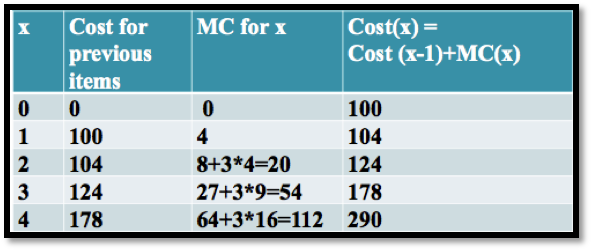
\includegraphics[width=\linewidth]{images/sec7-0-1.png}
\end{sbspanel}%
\end{sidebyside}%
\par
We would like to relate this data to the original graph of the marginal cost. When we consider this graph we see that the estimated cost actually corresponds to the area underneath the Marginal Cost function MC(x).%
\begin{sidebyside}{1}{0.2}{0.2}{0}%
\begin{sbspanel}{0.6}%
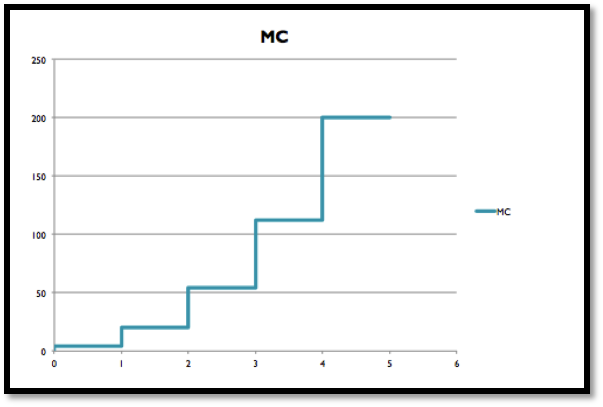
\includegraphics[width=\linewidth]{images/sec7-0-2.png}
\end{sbspanel}%
\end{sidebyside}%
\par
In other words, the cost function is the accumulation of the derivative (the marginal cost). Graphically, the cost function corresponds to the area underneath the marginal cost function.%
\par
We want to consider the accumulation of continuous functions.  In the language of calculus this is called finding an integral.%
\end{introduction}%
%
%
\typeout{************************************************}
\typeout{Section 1.1 Approximating Definite Integrals as Sums}
\typeout{************************************************}
%
\begin{sectionptx}{Approximating Definite Integrals as Sums}{}{Approximating Definite Integrals as Sums}{}{}{x:section:sec-7-1-RiemannSums}
\href{./Examples/Section-7-1-Examples.xlsx}{Link to worksheets used in this section}%
\par
The standard approach to accumulation is to reduce the problem to an area problem.  If we let f(t) be a velocity function, then the area under the y=f(t) curve between a starting value of t=a and a stopping value of t=b is the distance traveled in that time period.  In the easiest case, the velocity is constant and we use the simple formula%
%
\begin{equation*}
distance = velocity * time 
\end{equation*}
\begin{example}{Distance with Constant Speed.}{g:example:idm291770756960}%
Find the distance traveled if I go 60 mph from 12:30 until 3:00.%
\par
This problem is easy to do without any calculus.  If we graph the velocity function%
\begin{sidebyside}{1}{0.2}{0.2}{0}%
\begin{sbspanel}{0.6}%
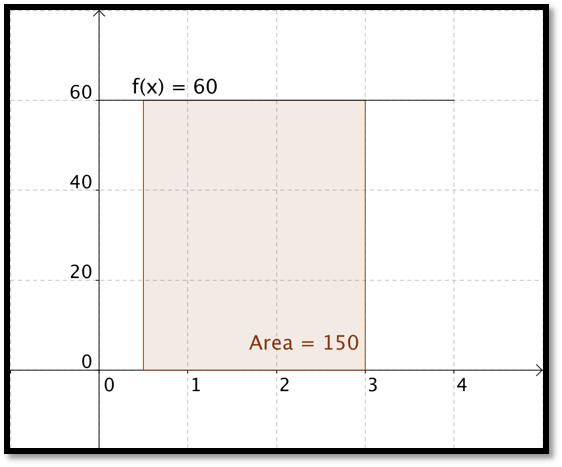
\includegraphics[width=\linewidth]{images/sec7-1-1.png}
\end{sbspanel}%
\end{sidebyside}%
\par
we find the area of the rectangle by taking base times height and noting \(60*(3-0.5)=150\).  Note that we do the same computation if I ask how much I earn over a period of 2.5 years if I make \textdollar{}60K a year, or how much oil is produced in 2 and a half hours form an oil well that produces 60 barrels of oil an hour.%
\end{example}
In a similar manner, if the function I am accumulating is linear, I can find area by using the area formula of a triangle, one half base time height.  The question becomes more difficult when I want to find the area under a curve that is not linear.  Suppose for example that we want to find the area under the curve%
%
\begin{equation*}
y = x * (4-x)
\end{equation*}
between x=0 and x=4.%
\begin{sidebyside}{1}{0.2}{0.2}{0}%
\begin{sbspanel}{0.6}%
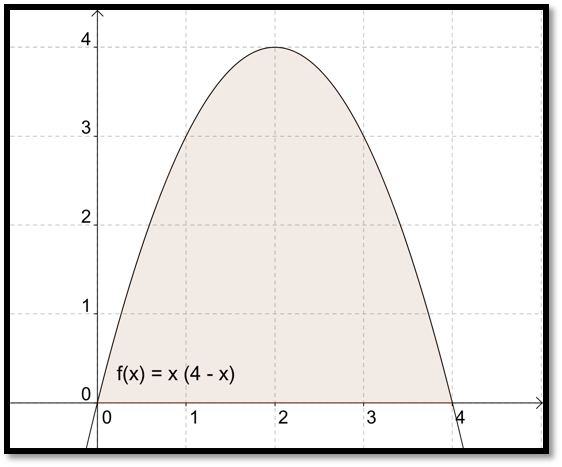
\includegraphics[width=\linewidth]{images/sec7-1-2.png}
\end{sbspanel}%
\end{sidebyside}%
\par
We no longer have a nice formula from geometry for the area.  Thus we start making approximations.  The easiest approximation is to note that the area has to be less than the area of the 4 by 4 rectangle we can draw around the region.%
\begin{sidebyside}{1}{0.2}{0.2}{0}%
\begin{sbspanel}{0.6}%
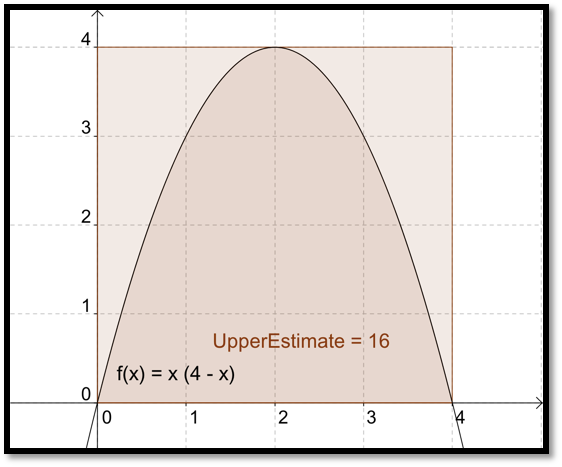
\includegraphics[width=\linewidth]{images/sec7-1-3.png}
\end{sbspanel}%
\end{sidebyside}%
\par
We can improve our estimate by dividing the interval [0, 4] into 4 equal subintervals and then taking the combined area of the 4 rectangles we need to contain the region.  This reduces our upper estimate from 16 to 14.%
\begin{sidebyside}{1}{0.2}{0.2}{0}%
\begin{sbspanel}{0.6}%
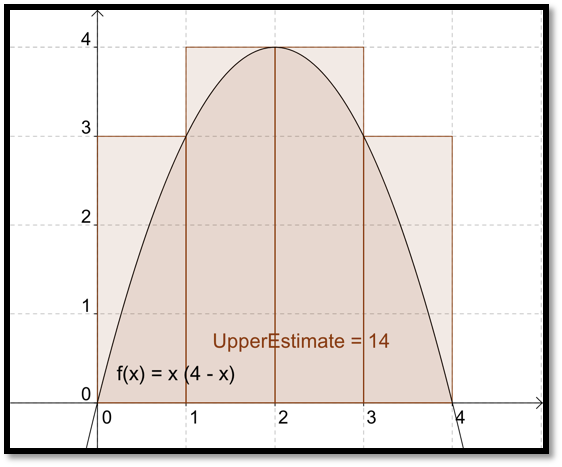
\includegraphics[width=\linewidth]{images/sec7-1-4.png}
\end{sbspanel}%
\end{sidebyside}%
\par
Similarly we could get a better estimate by looking at 8 subintervals and seeing that the area under the parabola is no more than 12.5%
\begin{sidebyside}{1}{0.2}{0.2}{0}%
\begin{sbspanel}{0.6}%
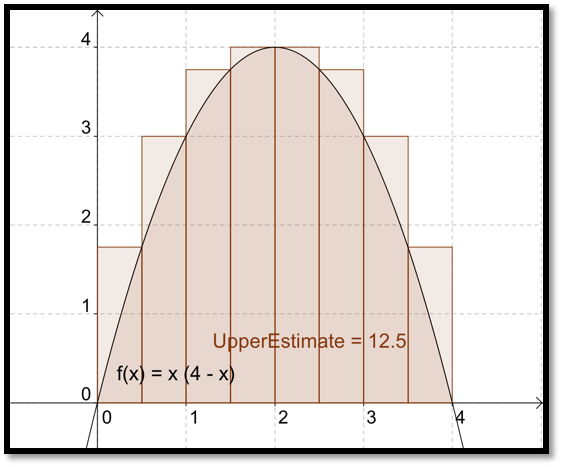
\includegraphics[width=\linewidth]{images/sec7-1-5.png}
\end{sbspanel}%
\end{sidebyside}%
\par
If we continue the process with 100 subintervals, our estimate is down to 10.83.  From the picture, it looks like a fairly good estimate.%
\begin{sidebyside}{1}{0.2}{0.2}{0}%
\begin{sbspanel}{0.6}%
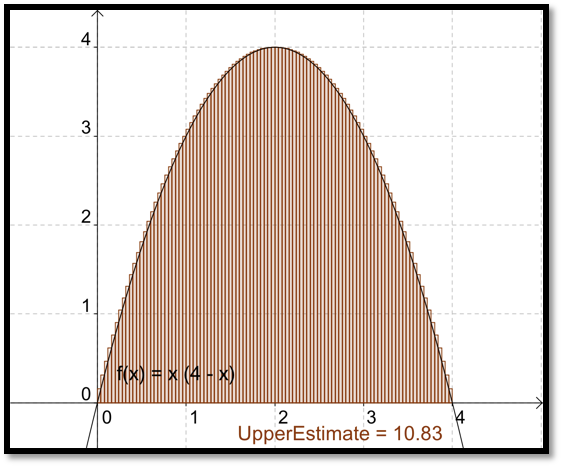
\includegraphics[width=\linewidth]{images/sec7-1-6.png}
\end{sbspanel}%
\end{sidebyside}%
\par
While this process would be very long and tedious by hand, the process of finding the area of each of 100 rectangles and adding the areas is rather easy in Excel.  Before going to Excel, we want to make a small adjustment in our method.  The method we used always gives an overestimate.  It also requires that we know where the function reaches a maximum on each subinterval.  It will be easier if we estimate area by always taking the height of the rectangle at the right end of the subinterval.  With 4 subintervals this gives an estimate of 10 for our area.%
\begin{sidebyside}{1}{0.2}{0.2}{0}%
\begin{sbspanel}{0.6}%
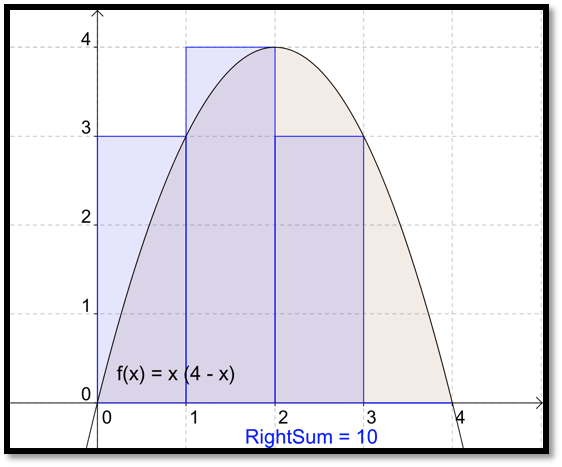
\includegraphics[width=\linewidth]{images/sec7-1-7.png}
\end{sbspanel}%
\end{sidebyside}%
\par
When we increase the number of subintervals to 100, we once again get a fairly good estimate of the area.  From the picture, it is hard to see difference between the area defined by the curve and the area defined by the rectangles.%
\begin{sidebyside}{1}{0.2}{0.2}{0}%
\begin{sbspanel}{0.6}%
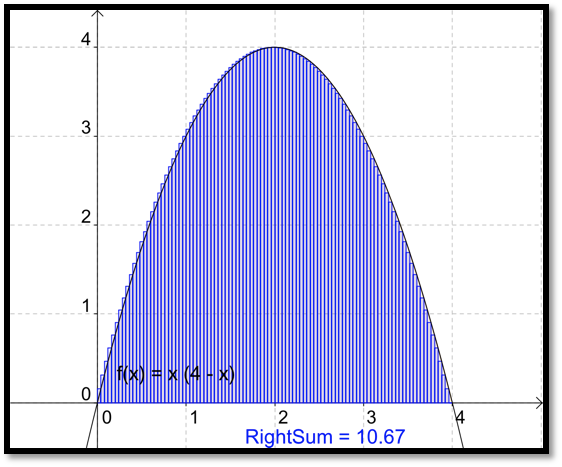
\includegraphics[width=\linewidth]{images/sec7-1-8.png}
\end{sbspanel}%
\end{sidebyside}%
\begin{example}{Approximating an Area with a Riemann Sum.}{x:example:area-parabola-down}%
Find the area under the curve \(y=x*(4-x)\) with \(x\) between 0 and 4 with Excel%
\par
We will approximate the area with 100 rectangles.  We set up a worksheet to find the area of the first rectangle.%
\begin{sidebyside}{1}{0.15}{0.15}{0}%
\begin{sbspanel}{0.7}%
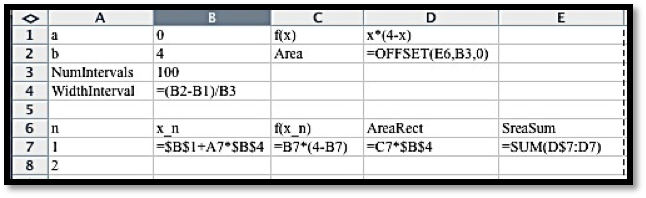
\includegraphics[width=\linewidth]{images/sec7-1-9.png}
\end{sbspanel}%
\end{sidebyside}%
\par
Following our standard practice, we set up the question and answer in labeled areas at the top of the worksheet.  The width of a subinterval is the width of the whole interval divided by the number of subintervals.  The column \(x_n\) is for the x value at the right side of the n-th subinterval.   The value of \(x_n\) is the starting point plus n times the width of a subinterval.  We then evaluate the function at \(x_n\).  The area of the n-th rectangle is the height, or \(f(x_n)\), times the width of the subinterval.  The last column is the total area for the first n rectangles.  The area for 100 rectangles is our area estimate.%
\par
To find the area we quick fill our worksheet.%
\begin{sidebyside}{1}{0.25}{0.25}{0}%
\begin{sbspanel}{0.5}%
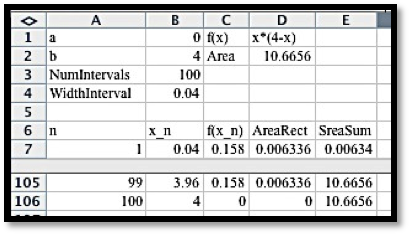
\includegraphics[width=\linewidth]{images/sec7-1-10.png}
\end{sbspanel}%
\end{sidebyside}%
\par
For a more accurate estimate we divide into smaller rectangles.%
\begin{sidebyside}{1}{0.25}{0.25}{0}%
\begin{sbspanel}{0.5}%
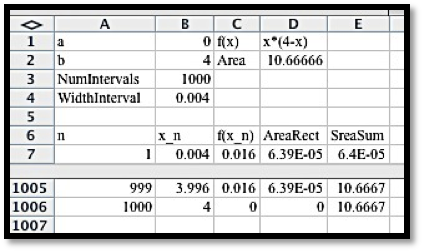
\includegraphics[width=\linewidth]{images/sec7-1-11.png}
\end{sbspanel}%
\end{sidebyside}%
\end{example}
While 100 subintervals will be close enough for most of the problems we are interested is, the "area", or definite integral will be defined as the limit of this sum as the number of subintervals goes to infinity.  Thus%
\begin{assemblage}{}{g:assemblage:idm291770856640}%
%
\begin{equation*}
\int_a^bf(x)  dx=\lim_{n\to \infty} \sum_{i=1}^nf (x_i)\Delta x 
\end{equation*}
%
\par
with \(\Delta x=\frac{b-a}{n}\)  and  \(x_i=a+i*\Delta x\).%
\end{assemblage}
The sums of the form, \(\sum_{i=1}^n  f(x_i)\Delta x\) with \(\Delta x=\frac{b-a}{n}\) and \(x_i=a+i*\Delta x\), are called \terminology{Riemann sums}.  The limit, written \(\int_a^bf(x)  dx\), is called a \terminology{definite integral}.%
\par
As a memory aid, it is worth noting that the symbol used for the sum is an upper case sigma, or S for sum in the Greek alphabet.  When we take the limit we use an integral sign, which is a stylized S in the Latin alphabet.%
\par
It is worth noting that in this definition we are finding “signed area under a curve.”  If the function \(f(x)\) is negative over the interval, the integral will also be negative, in the same we would have a negative change in our bank statement if we were steadily removing money.  Similarly we can get a negative integral when the ends of the interval are reversed.  If I am steadily adding money to an account, the net change is negative if I measure from 5 years in the future back to today.%
\par
We should note that, for functions nice enough to be considered in this class, we get to the same limit by using rectangles with the function evaluated on the right side of the rectangle or the left side of the rectangle, or any point in the rectangle we choose.  Choosing the right hand side for evaluation makes our formulas a little simpler.%
\begin{example}{Present Value of a Revenue Stream.}{g:example:idm291770872496}%
The estimated current value of the revenue stream, in billions of dollars, of a company being bought out is \(f(x)=\exp(-0.06*x)*0.235\). The present value of that revenue stream is the area of the region under the curve \(y=f(x)\) from \(x=0\) to \(x=15\).  Use 500 intervals to estimate the present value.%
\par
Although the data in the question for this example is quite different from the previous example, the setup for the worksheet to evaluate the Riemann sum is the same.%
\begin{sidebyside}{1}{0.1}{0.1}{0}%
\begin{sbspanel}{0.8}%
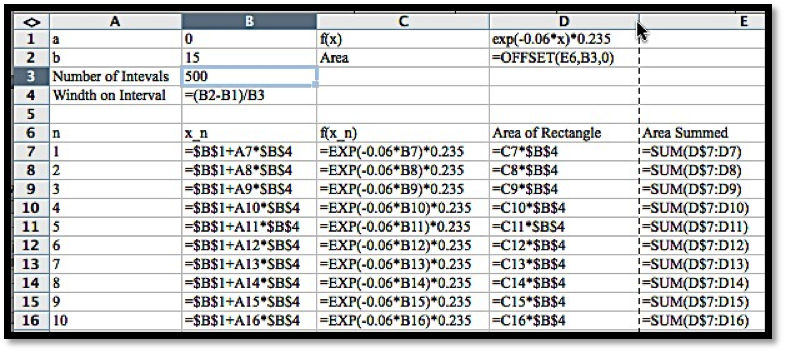
\includegraphics[width=\linewidth]{images/sec7-1-12.png}
\end{sbspanel}%
\end{sidebyside}%
\par
With 500 intervals we estimate the present value of the revenue stream to be worth \textdollar{}2.3222 Billion.  If we had only used 100 intervals, the estimate would have been for \textdollar{}2.318 Billion, while 1000 intervals gives an estimate of \textdollar{}2.3232 Billion.%
\end{example}
%
%
\typeout{************************************************}
\typeout{Exercises 1.1.1 Exercises: Approximating Definite Integrals as Sums Problems}
\typeout{************************************************}
%
\begin{exercises-subsection}{Exercises: Approximating Definite Integrals as Sums Problems}{}{Exercises: Approximating Definite Integrals as Sums Problems}{}{}{x:exercises:exercises-set-sec-7-1}
\begin{divisionexercise}{1}{}{}{g:exercise:idm291770913312}%
Let \(f(x) = 4 x + 5\).  Estimate the area under \(f(x)\) on the interval \(0 \le  x \lt 7\) using 100 rectangles and a right hand rule.%
\par\smallskip%
\noindent\textbf{Solution}.\hypertarget{g:solution:idm291770916336}{}\quad{}The Excel commands are:%
\begin{sidebyside}{1}{0}{0}{0}%
\begin{sbspanel}{1}%
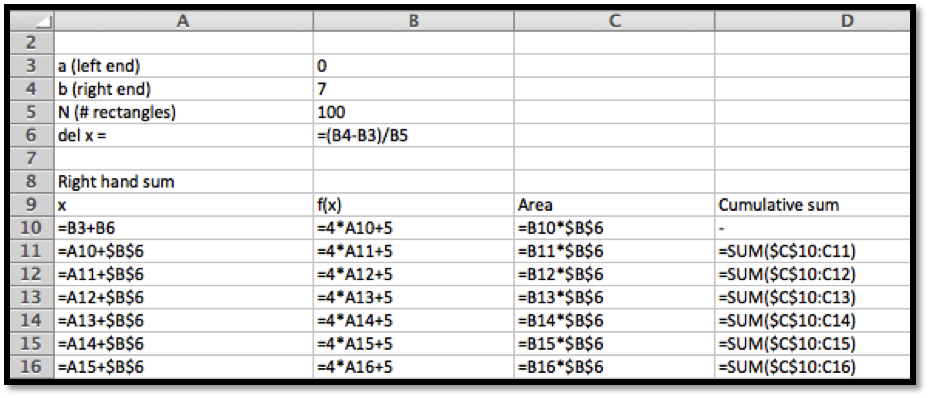
\includegraphics[width=\linewidth]{images/sec7-1-sol1a.png}
\end{sbspanel}%
\end{sidebyside}%
\par
The answer is given as follows. Note that in this screen grab the center part of the sidebyside was hidden so that the image is a reasonable size%
\par
The area is approximately 133.98%
\begin{sidebyside}{1}{0.2}{0.2}{0}%
\begin{sbspanel}{0.6}%
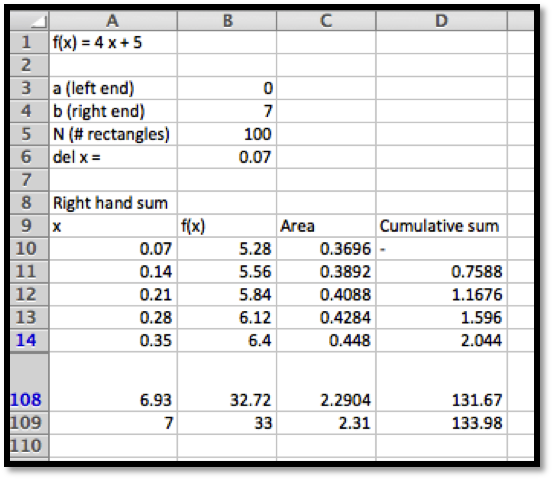
\includegraphics[width=\linewidth]{images/sec7-1-sol1b.png}
\end{sbspanel}%
\end{sidebyside}%
\end{divisionexercise}%
\begin{divisionexercise}{2}{}{}{g:exercise:idm291770926480}%
Let \(f(x) = 5 – 3 x\).  Estimate the area under \(f(x)\) on the interval \(2 \le  x \lt 10\) using 200 rectangles and a right hand rule.%
\end{divisionexercise}%
\begin{divisionexercise}{3}{}{}{g:exercise:idm291770924640}%
Let \(f(x) = x^2  + 3 x + 1\).  Estimate the area on the interval \(-10\le  x \lt -2\) under \(f(x)\) using 200 rectangles and a right hand rule.%
\par\smallskip%
\noindent\textbf{Solution}.\hypertarget{g:solution:idm291770963840}{}\quad{}The set-up is very similar to the one in problem 1.%
\begin{sidebyside}{1}{0}{0}{0}%
\begin{sbspanel}{1}%
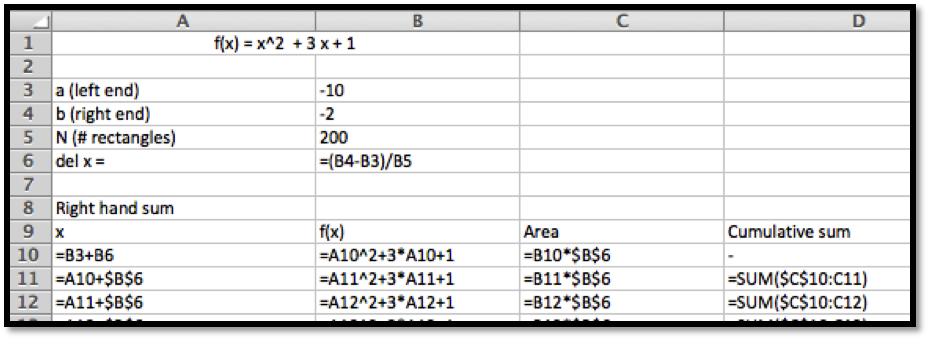
\includegraphics[width=\linewidth]{images/sec7-1-sol3a.png}
\end{sbspanel}%
\end{sidebyside}%
\par
The area underneath the curve is approximately 193.228 according to the Excel computation.%
\begin{sidebyside}{1}{0.2}{0.2}{0}%
\begin{sbspanel}{0.6}%
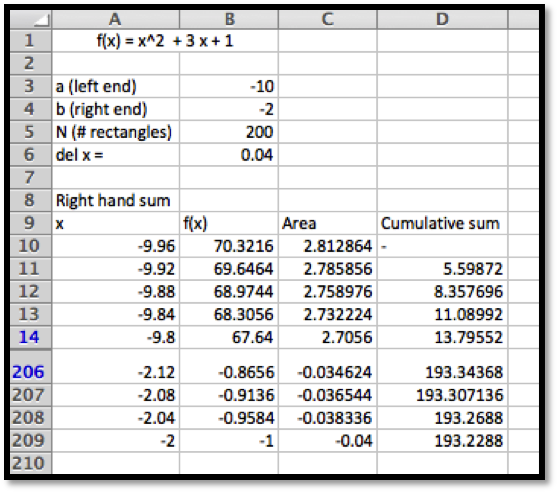
\includegraphics[width=\linewidth]{images/sec7-1-sol3b.png}
\end{sbspanel}%
\end{sidebyside}%
\end{divisionexercise}%
\begin{divisionexercise}{4}{}{}{g:exercise:idm291770006704}%
Let \(f(x) = -x^2  + 7 x - 10\).  Estimate the area below the curve \(y =  f(x)\) and above the x-axis using 100 rectangles and a right hand rule.%
\end{divisionexercise}%
\begin{divisionexercise}{5}{}{}{g:exercise:idm291770005216}%
Let \(f(x) = 3 \ln(x)\).  Estimate the area under \(f(x)\) on the interval \(1 \le  x \lt 10\) using 50 rectangles and a right hand rule.%
\par\smallskip%
\noindent\textbf{Solution}.\hypertarget{g:solution:idm291770003504}{}\quad{}\begin{sidebyside}{1}{0.25}{0.25}{0}%
\begin{sbspanel}{0.5}%
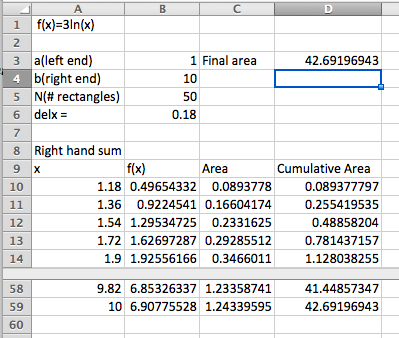
\includegraphics[width=\linewidth]{images/sec7-1-sol5a.png}
\end{sbspanel}%
\end{sidebyside}%
\par
A set-up similar to the one in problems 1 and 3 gives us an approximation for the area of  42.69.%
\end{divisionexercise}%
\begin{divisionexercise}{6}{}{}{g:exercise:idm291770001184}%
Let \(f(x) = x \exp(-0.7 x)\).  Estimate the area on the interval \(1 \le  x \lt 5\) under \(f(x)\) using 100 rectangles and a right hand rule.%
\end{divisionexercise}%
\begin{divisionexercise}{7}{}{}{g:exercise:idm291769999296}%
Let \(f(x) = (5 x + 3) \exp(-0.7 x)\).  Estimate the area under \(f(x)\) on the interval \(0 \le  x \lt 5\) using 100 rectangles and a right hand rule.%
\par\smallskip%
\noindent\textbf{Solution}.\hypertarget{g:solution:idm291769997584}{}\quad{}\begin{sidebyside}{1}{0.2}{0.2}{0}%
\begin{sbspanel}{0.6}%
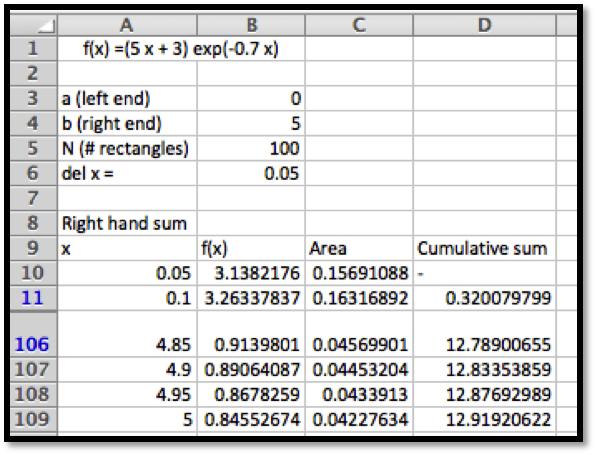
\includegraphics[width=\linewidth]{images/sec7-1-sol7a.png}
\end{sbspanel}%
\end{sidebyside}%
\par
The area underneath the curve is approximately 12.92%
\end{divisionexercise}%
\begin{divisionexercise}{8}{}{}{g:exercise:idm291769995312}%
Consider the area under the line \(y = 5 x + 7\) on the interval \(1 \le  x \le  5\).%
%
\begin{enumerate}[label=(\alph*)]
\item{}Using only what you know about areas of rectangles and triangles, find the exact area.%
\item{}Find the approximations to the area using Riemann sums with 50, 100, and 200 intervals.%
\item{}Find the error for each of the three approximations you made.%
\item{}For this case, make an estimate of the error in terms of the number of intervals used.%
\end{enumerate}
\end{divisionexercise}%
\begin{divisionexercise}{9}{}{}{g:exercise:idm291769990720}%
Consider the area under the line \(y = x^2\) on the interval \(0 \le  x \le  3\).  In later sections we will show that the exact area is 9.%
%
\begin{enumerate}[label=(\alph*)]
\item{}Find the approximations to the area using Riemann sums with 1, 10, 100, and 1000 intervals.%
\item{}Find the error for each of the four approximations you made.%
\item{}For this case, make an estimate of the error in terms of the number of intervals used.%
\item{}How many intervals would we need for an error of less that \(10^{-6}\)?%
\end{enumerate}
\par\smallskip%
\noindent\textbf{Solution}.\hypertarget{g:solution:idm291769985840}{}\quad{}%
\begin{enumerate}[label=(\alph*)]
\item{}\begin{sidebyside}{1}{0}{0}{0}%
\begin{sbspanel}{1}%
{\centering%
{\tabularfont%
\begin{tabular}{ccc}\hrulethick
N&Riemann Sum&Error\tabularnewline\hrulethin
1&27&18\tabularnewline\hrulethin
10&10.395&1.395\tabularnewline\hrulethin
100&9.135&0.135\tabularnewline\hrulethin
1000&9.0135&0.0135\tabularnewline\hrulethin
\end{tabular}
}%
\par}
\end{sbspanel}%
\end{sidebyside}%
%
\item{}The errors are included in the sidebyside above. Subtract 9 from the approximation found in Excel.  Note that there is a bit of a pattern.%
\item{}The larger values of N seem to have an error of about \(\frac{13.5}{N}\)%
\item{}If  error \(\lt 10^{-6}\). Then \(\frac{13.5}{N}\lt 10^{-6}\). Then \(\frac{N}{13.5}\gt 1,000,000\), and hence \(N\gt 13,500,000\).%
\end{enumerate}
\end{divisionexercise}%
\begin{divisionexercise}{10}{}{}{g:exercise:idm291769970848}%
You have a natural gas well.  You have been told that as gas is extracted and the pressure in the well lessens, the rate of extraction also decreases. The weekly production is \(10000 \exp(-0.01 t)\) cubic feet per week.%
%
\begin{enumerate}[label=(\alph*)]
\item{}Estimate the production in the first year.%
\item{}Estimate the production in the third year.%
\end{enumerate}
\end{divisionexercise}%
\begin{divisionexercise}{11}{}{}{g:exercise:idm291769967776}%
Sales of your new gadget are estimated at \(500*2^{.08 t}\) units per month.%
%
\begin{enumerate}[label=(\alph*)]
\item{}Estimate the total sales in the first year.%
\item{}Estimate the total sales in the fourth year.%
\item{}Estimate the total sales over the first 5 years.%
\end{enumerate}
\par\smallskip%
\noindent\textbf{Solution}.\hypertarget{g:solution:idm291769964400}{}\quad{}%
\begin{enumerate}[label=(\alph*)]
\item{}Estimate the total sales in the first year.%
\par
The total sales would be the sum of the sales each month. This is the same as a right hand sum of the function \(Sales(t)= 500*2^{.08 t}\) on the interval [0,12] with 12 subdivisions. The Excel commands are as follows (quick fill down to complete the Excel table)%
\begin{sidebyside}{1}{0.1}{0.1}{0}%
\begin{sbspanel}{0.8}%
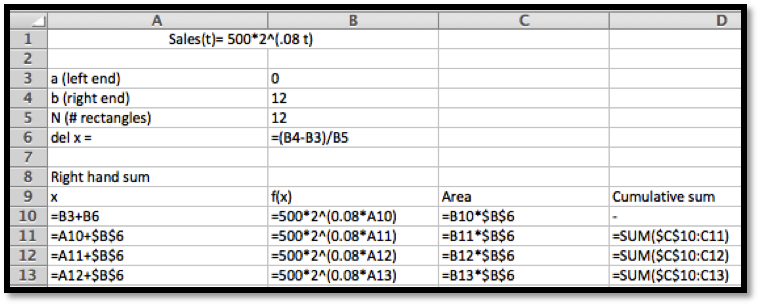
\includegraphics[width=\linewidth]{images/sec7-1-sol11a.png}
\end{sbspanel}%
\end{sidebyside}%
\par
Results:%
\begin{sidebyside}{1}{0.25}{0.25}{0}%
\begin{sbspanel}{0.5}%
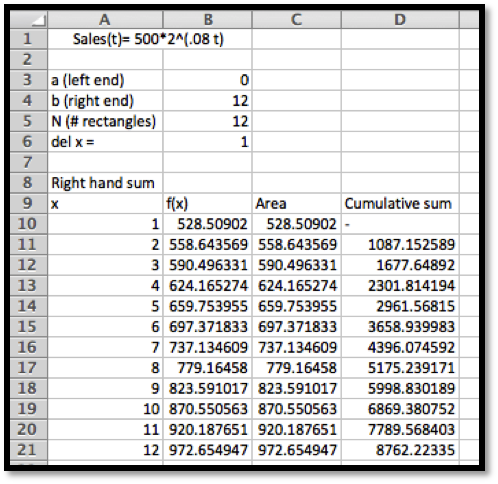
\includegraphics[width=\linewidth]{images/sec7-1-sol11b.png}
\end{sbspanel}%
\end{sidebyside}%
\par
So the total sales is \textdollar{}8,762.22%
\item{}Estimate the total sales in the fourth year.%
\par
We need to adjust the computation so that the sales added correspond to the sales of the fourth year only. This would be from month 36 to 48. We can just adjust the values in the EXCEL table above!%
\begin{sidebyside}{1}{0.25}{0.25}{0}%
\begin{sbspanel}{0.5}%
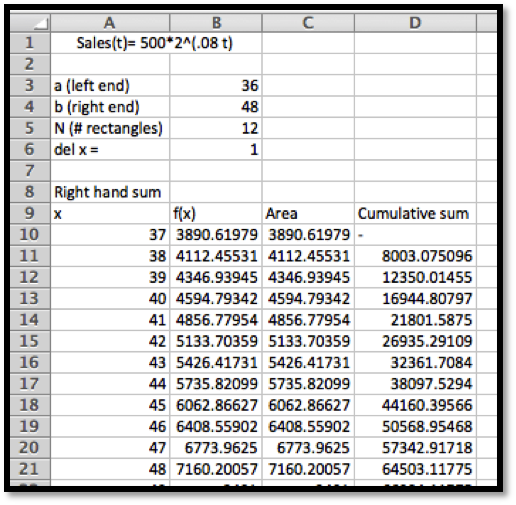
\includegraphics[width=\linewidth]{images/sec7-1-sol11c.png}
\end{sbspanel}%
\end{sidebyside}%
\par
So the total sales in the fourth year are \textdollar{}64,503.12%
\item{}Estimate the total sales over the first 5 years.%
\par
This will be a much larger range. We will add the sales for the first 5 years. In other words: the first 60 months. Note that this means we want to change \(N\) to 60 (we want to do the computation for each month) The rows from 13 to 65 have been hidden from views to create a smaller size image for this solution manual:%
\begin{sidebyside}{1}{0.15}{0.15}{0}%
\begin{sbspanel}{0.7}%
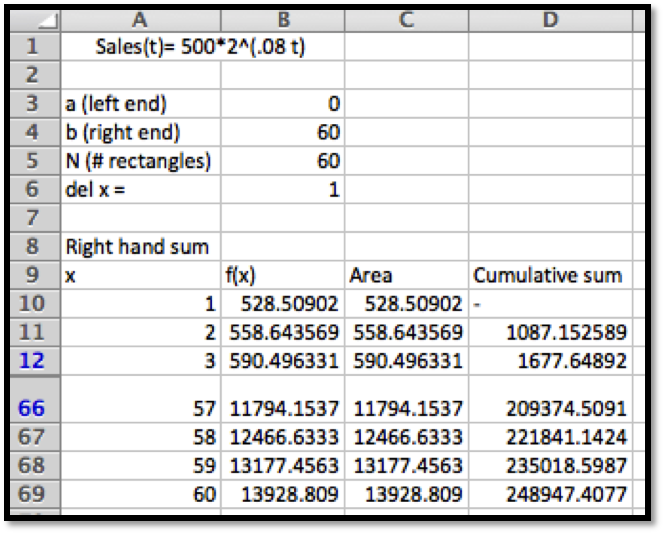
\includegraphics[width=\linewidth]{images/sec7-1-sol11d.png}
\end{sbspanel}%
\end{sidebyside}%
\par
The total sales for the first 5 years is \textdollar{}248,947.41%
\end{enumerate}
\end{divisionexercise}%
\begin{divisionexercise}{12}{}{}{g:exercise:idm291769951200}%
You run a low cost, high volume widget manufacturing plant.  For reports, you write your reports in terms of millions of units.  When measured in units of one million widgets and one million dollars, the marginal profit function is \(p(x) = -1 + 10 x – x^2\).%
%
\begin{enumerate}[label=(\alph*)]
\item{}Find the profit from making 12 million widgets.%
\item{}What quantities have 0 marginal profit?%
\item{}What is the maximum profit to be made manufacturing widgets?%
\end{enumerate}
\end{divisionexercise}%
\end{exercises-subsection}
\end{sectionptx}
%
%
\typeout{************************************************}
\typeout{Section 1.2 The Fundamental Theorem of Calculus}
\typeout{************************************************}
%
\begin{sectionptx}{The Fundamental Theorem of Calculus}{}{The Fundamental Theorem of Calculus}{}{}{x:section:sec-7-2-FundamentalTheoremCalculius}
\href{./Examples/Section-7-2-Examples.xlsx}{Link to worksheets used in this section}%
\par
In the last section we defined the definite integral, \(\int_a^b f(t)dt\), the signed area under the curve \(y= f(t)\) from \(t=a\) to \(t=b\), as the limit of the area found by approximating the region with thinner and thinner rectangles.  We also saw that we can easily find a reasonable approximation to the area using Excel to find such a sum with a fairly large number of rectangles.%
\par
In the trivial case where we have a constant function \(f(t)=c\) we can find the area of the area with a simple formula, \(\int_a^bc dt=c(b-a)=cb-ca\). If we define an area function, \(F(x)\), as the area under the curve \(y=f(t)\) from \(t=0\) to \(t=x\), then the area function in this case is  \(F(x)=c*x\).  We would like to be able to evaluate more integrals with a process like this, where we have a simple area function.%
\begin{remark}{Note on variables used.}{g:remark:idm291769939632}%
We shifted the independent variable from \(t\) for the function \(f\) to \(x\) for the function \(F\) because we have two independent variables in our discussion and we want to keep them separate to avoid confusion.  We will consider \(f\) as a function of \(t\), and want to find the area under the graph of \(f(t)\).  We will consider \(F\) as a function of \(x\), and understand it as the area under the curve \(y=f(t)\) from some starting point \(t=a\) to \(t=x\).%
\end{remark}
We start by exploring cases where we can justify an area function without using calculus.  We will then look at some cases where we can experimentally verify the area function with Excel.  Finally we will give the general rule for the area function, the Fundamental Theorem of Calculus, and will give some justification.%
\begin{example}{Area function for constant by geometry.}{g:example:idm291741605248}%
Let \(f(t)=c\).  For a constant function, \(f(t)=c\), the area under the curve will be the area of a rectangle of height \(c\) and width \(b-a\).  The obvious area function is \(F(x)=c*x\).  Then%
%
\begin{equation*}
\int_a^b c dt=F(b)-F(a)=c*b-c*a=c(b-a).
\end{equation*}
It is worth noting that this formula gives "signed area."  If c or b-a is negative, the "area" is negative.%
\begin{sidebyside}{1}{0.2}{0.2}{0}%
\begin{sbspanel}{0.6}%
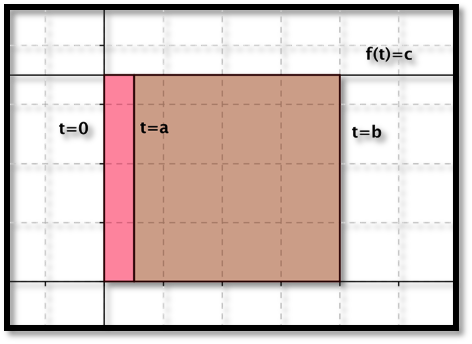
\includegraphics[width=\linewidth]{images/sec7-2-1.png}
\end{sbspanel}%
\end{sidebyside}%
\end{example}
\begin{example}{Area function for linear function by geometry.}{g:example:idm291741599744}%
Let \(f(t) = c*t\).  For a linear function, \(f(t) = c*t\), the area under the curve from 0 to \(b\) will be the area of a triangle of height \(c*b\) and width \(b\).%
\begin{sidebyside}{1}{0.2}{0.2}{0}%
\begin{sbspanel}{0.6}%
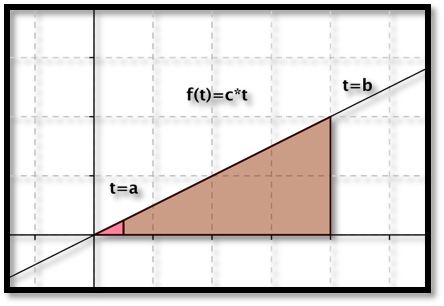
\includegraphics[width=\linewidth]{images/sec7-2-2.png}
\end{sbspanel}%
\end{sidebyside}%
\par
The obvious area function is \(F(x)=c*x^2/2\).  If \(a\) is also nonzero, the area is the difference of the areas of two triangles.%
%
\begin{equation*}
\int_a^b c*t dt=F(b)-F(a)=
\frac{c*b^2}{2}-\frac{c*a^2}{2}=\frac{c (b^2-a^2 )}{2}.
\end{equation*}
\end{example}
\begin{remark}{A note on versions of Riemann sum used.}{g:remark:idm291741593344}%
As we consider finding area with Excel and Riemann sums, rather than use a right-hand rule for the rectangles, we are going to use a midpoint rule where we find the area of rectangles evaluated at the middle of each interval.%
\begin{sidebyside}{1}{0.2}{0.2}{0}%
\begin{sbspanel}{0.6}%
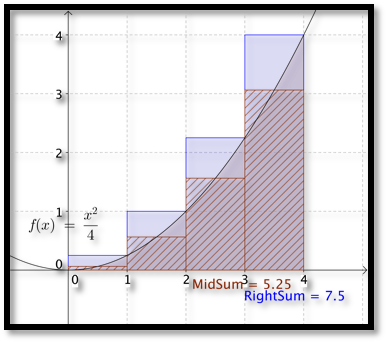
\includegraphics[width=\linewidth]{images/sec7-2-3.png}
\end{sbspanel}%
\end{sidebyside}%
\par
The right-hand rule uses an easier formula, so we used it first.  For the ith rectangle we evaluate at \(x_i=a+i\Delta x\).  For the midpoint formula, we evaluate at the midpoint of the interval, at \(mid_i=a+i\Delta x-\Delta x/2\).  As the picture suggests, the midpoint formula gives a better approximation.  The right-hand rule always overestimates an increasing function.  The midpoint rule is exact for linear functions where the midpoint is the average value.%
\end{remark}
In both of the examples we have examined the area function has the original function as its derivative.  We would like to use Excel to test a few more cases. In the worksheets we set up in the last section, SumArea is the area function we are looking for.  We will plot the area function and use a best-fit curve to find the equation of the area function.%
\begin{example}{Best fitting area function for a linear function.}{g:example:idm291741588128}%
Repeat the last example, finding the area under \(f(x)=6x\), with Excel.  With a linear function we have use the following to produce an area function.%
\begin{sidebyside}{1}{0.05}{0.05}{0}%
\begin{sbspanel}{0.9}%
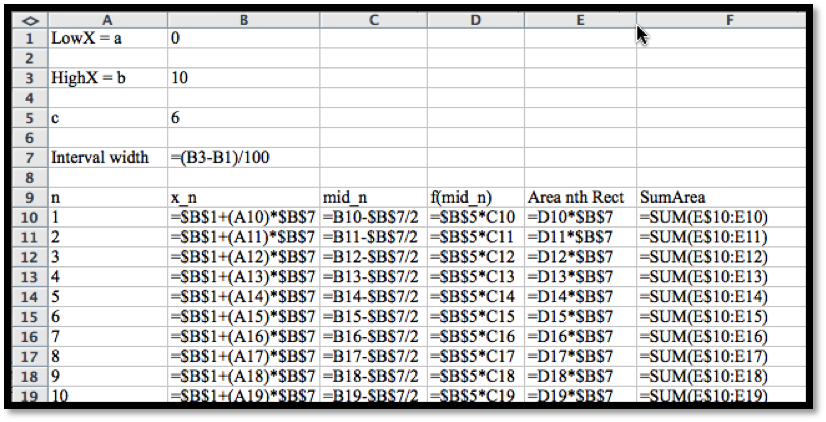
\includegraphics[width=\linewidth]{images/sec7-2-4.png}
\end{sbspanel}%
\end{sidebyside}%
\par
Column C has our list of \(t\) values in the center of each interval.  Column D has the value of \(f(t)\) evaluated at those points.  The area of the rectangle is the height \(f(mid_n)\) times the width, Interval width.  SumArea is our running area function.  When we plot the area function we have something that seems to be quadratic with leading coefficient \(c/2\) and very small linear and constant coefficients.  In fact the linear and constant coefficients are zero up to a rounding factor for numbers of the size we are using.%
\begin{sidebyside}{1}{0.1}{0.1}{0}%
\begin{sbspanel}{0.8}%
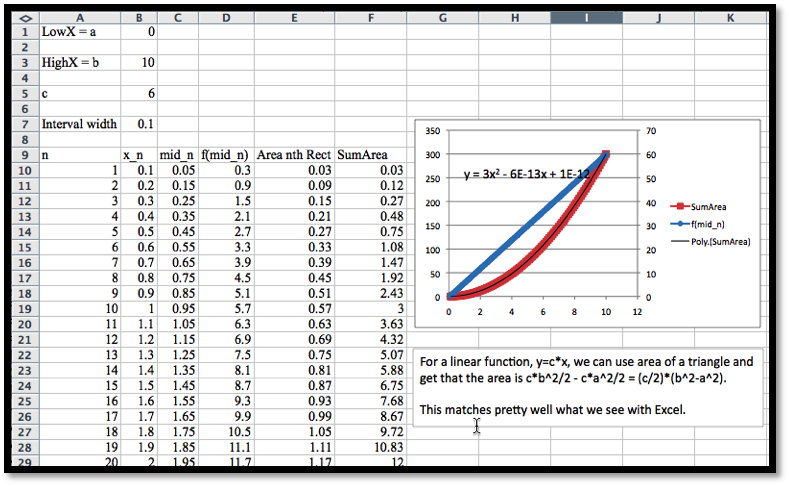
\includegraphics[width=\linewidth]{images/sec7-2-5.png}
\end{sbspanel}%
\end{sidebyside}%
\end{example}
 a This matches the result we had solving the problem with geometry.  However, we can repeat the process with Excel and use functions of higher order.%
\begin{example}{Best fitting area function for a quadratic function.}{g:example:idm291741580416}%
Find the area function when \(f(t) = 6t^2\).%
\par
For this problem we essentially repeat the work of the previous example with a quadratic function for \(f(t)\).%
\begin{sidebyside}{1}{0.05}{0.05}{0}%
\begin{sbspanel}{0.9}%
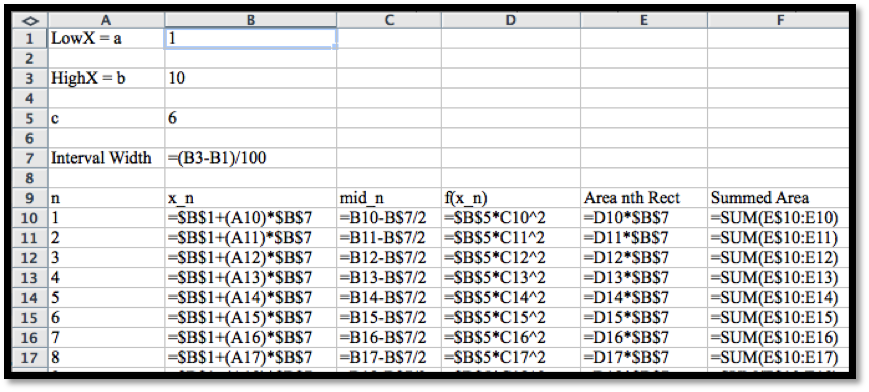
\includegraphics[width=\linewidth]{images/sec7-2-6.png}
\end{sbspanel}%
\end{sidebyside}%
\par
When we plot the area function we get a very good fit with a cubic function.  Once again, allowing for the way best-fit curves may return small random values for coefficients that should be zero, we see that if \(f(t) =c*t^2\), then the related area function is%
%
\begin{equation*}
F(x)=c*t^3/3\text{.}
\end{equation*}
\begin{sidebyside}{1}{0}{0}{0}%
\begin{sbspanel}{1}%
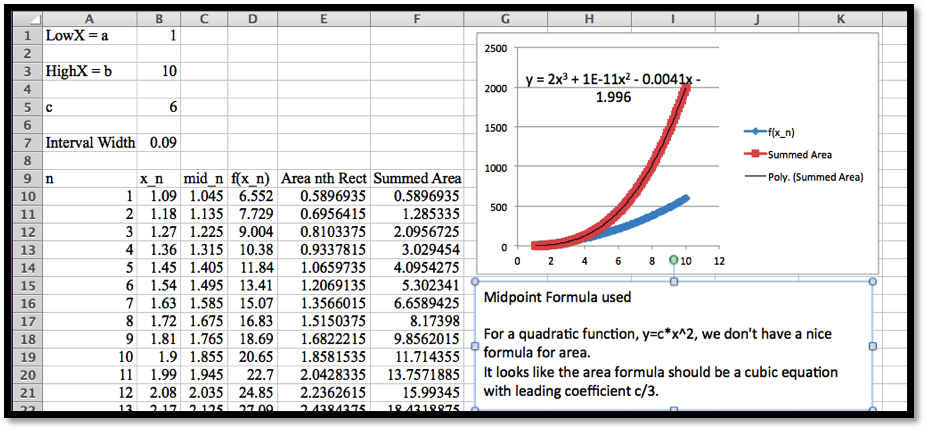
\includegraphics[width=\linewidth]{images/sec7-2-7.png}
\end{sbspanel}%
\end{sidebyside}%
\end{example}
\begin{example}{Best fitting area function for a cubic function.}{g:example:idm291741573232}%
Find the area when \(f(x)=6 x^3\).%
\par
Once again, we can use Excel to produce an area function.  The area function seems to be \(F(x)=1.5 x^4\).%
\begin{sidebyside}{1}{0}{0}{0}%
\begin{sbspanel}{1}%
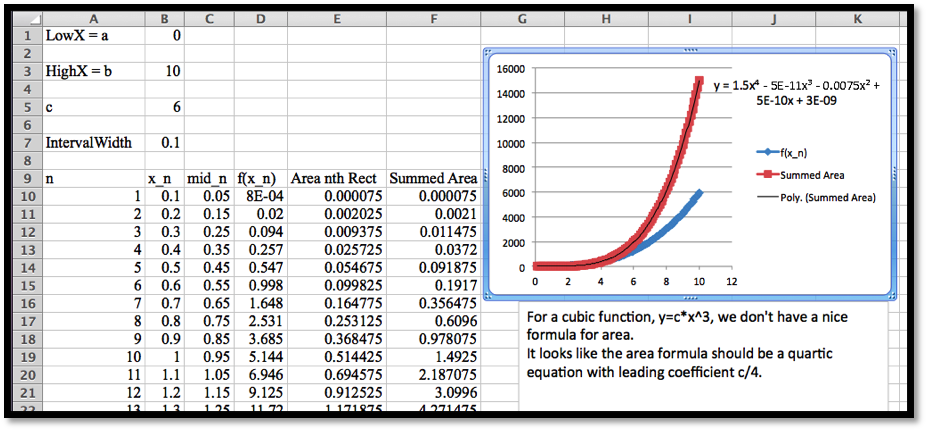
\includegraphics[width=\linewidth]{images/sec7-2-8.png}
\end{sbspanel}%
\end{sidebyside}%
\end{example}
In all the examples above we note that the area function, \(F(x)\),  has \(f(x)\), the curve we are finding the area under, as its derivative.  Thus, in these cases, the area is an anti-derivative of \(f(x)\).  This observation generalizes to the Fundamental Theorem of Calculus, which has two versions:%
\begin{assemblage}{}{g:assemblage:idm291741567248}%
\begin{theorem}{Fundamental Theorem of Calculus (first version).}{}{g:theorem:idm291741566848}%
Let \(f(x)\) be a continuous function on the interval \([a, b]\).  On that interval define an area function by \(F(x)=\int_a^x f(t)  dt\). Then \(\frac{d}{dx} F(x)=f(x)\).\end{theorem}
%
\end{assemblage}
\begin{assemblage}{}{g:assemblage:idm291741563952}%
\begin{theorem}{Fundamental Theorem of Calculus (second version).}{}{g:theorem:idm291741563552}%
Let \(f(x)\) be a continuous function on the interval \([a, b]\).  Suppose \(F(x)\) is any continuous,  differentiable function with \(\frac{d}{dx} F(x)=f(x)\).  Then \(\int_a^b f(t) dt=F(b)-F(a)\).\end{theorem}
%
\end{assemblage}
In practice we use the second version of the fundamental theorem to evaluate definite integrals.  We find a function \(F(x)\) whose derivative is the integrand \(f(x)\) and then evaluate \(F(x)\) at the endpoints. It is easier to prove or justify the first version of the fundamental theorem.  The basic argument notes that is \(F(x)=\int_a^xf(t) \ dt\), then formally%
%
\begin{equation*}
\frac{d}{dx} F(x)=\lim_{h\to 0}
\frac{(F(x+h)-F(x))}{h}.
\end{equation*}
\begin{sidebyside}{1}{0.15}{0.15}{0}%
\begin{sbspanel}{0.7}%
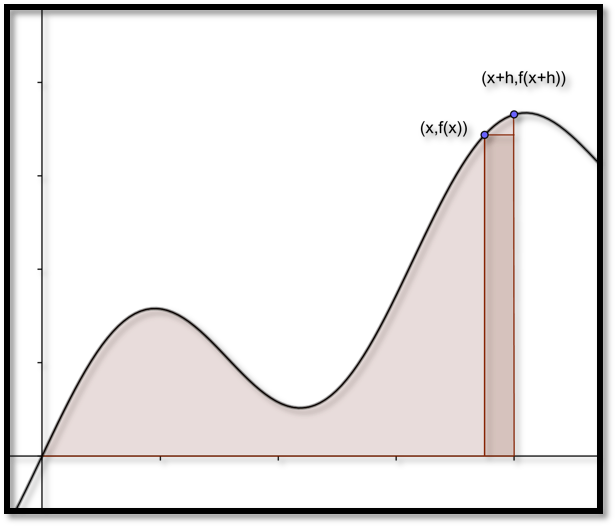
\includegraphics[width=\linewidth]{images/sec7-2-9.png}
\end{sbspanel}%
\end{sidebyside}%
\par
But if \(h\) is small, \(F(x+h)-F(x)\) is approximately the area of a rectangle of height \(f(x)\) and with \(h\), so the \(F'(x) = f(x)\).  We then note that any two anti-derivatives of a function differ by a constant.%
\begin{example}{Redoing an old area problem by the  FTC.}{g:example:idm291741553264}%
In \hyperref[x:example:area-parabola-down]{example~\ref{x:example:area-parabola-down}} in the previous section, we used Riemann sums with 100 and 1000 intervals to approximate the area under \(y = x*(4-x)\) with \(x\) between 0 and 4.  Find the area using the fundamental theorem of calculus,%
\par
We rewrite the curve as \(f(x) = 4x – x^2\) and note that one anti-derivative of \(f(x)\) is \(F(x) = 2 x^2 - x^3/3\).  Then%
%
\begin{equation*}
\int_0^4 f(x)\ dx=F(4)-F(0)=\left(32-\frac{64}{3}\right)-(0)=10 \frac{2}{3}.
\end{equation*}
\end{example}
To get the same answer to 4 decimal places, we needed to use 1000 intervals with Riemann sums.  Clearly, it is easier to solve this problem with the fundamental theorem of calculus than to make an approximation with that many intervals.%
\begin{example}{Verifying an antiderivative to find area.}{g:example:idm291741547744}%
Let \(f(x)=x^2 e^{-x}\).  We are told \(F(x)=(x^2+2 x+2) (-e^{-x})\)  is an anti-derivative of \(f(x)\).  Verify the anti-derivative and find the area under the curve with \(x\) between 0 and 2.%
\par
Using the product rule,%
%
\begin{equation*}
F'(x)=(2x+2) (-e^{-x}) + (x^2+2x+2) (e^{-x})=x^2 e^{-x}=f(x)
\end{equation*}
The area is%
%
\begin{equation*}
F(2) – F(0) = 10(-e^{-2}) – 2(e^{0}) = -2 – 10/e^2 = -3.3534
\end{equation*}
\end{example}
We also want to revisit our first three examples in light of the fundamental theorem if calculus.  In all of those examples we used Excel to find a best fitting curve for an area function.  We can now check our work by taking the derivative, adjusting parameters as needed to find an anti-derivative.  For constant and linear functions we have already done the adjusting because we could find the area function from geometry.%
\begin{example}{Using the FTC to guess and check area under a quadratic.}{g:example:idm291741542352}%
Example 3a: Find the area function when \(f(t) = 6t^2\).%
\par
We have already used Excel to find a best fitting curve.%
\begin{sidebyside}{1}{0}{0}{0}%
\begin{sbspanel}{1}%
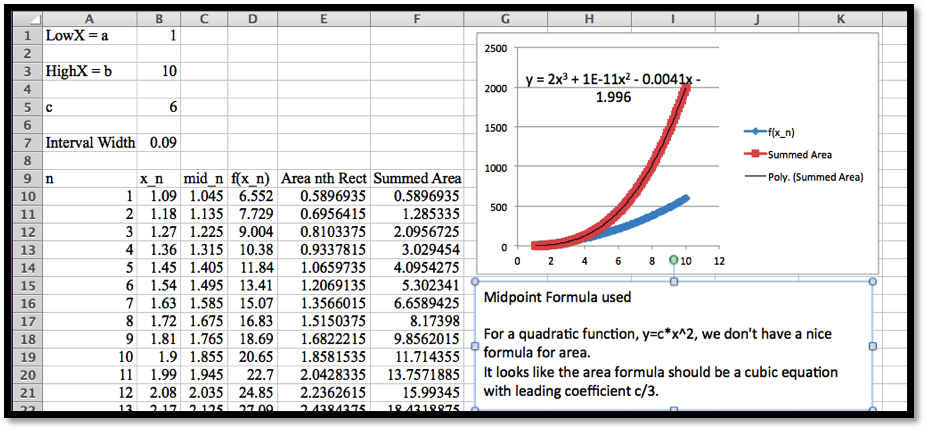
\includegraphics[width=\linewidth]{images/sec7-2-10.png}
\end{sbspanel}%
\end{sidebyside}%
\par
We are thus suspicious that the anti-derivative should be a cubic polynomial.  We need%
%
\begin{equation*}
6t^2=d/dt (at^3+bt^2+ct+d)=3at^2+2bt+c.
\end{equation*}
Setting coefficients equal for each power, we see \(a = 2\) and \(b = c = 0\).  Thus our area function has the form \(F(t) = 2 t^3 + d\).  Since \(F(0)\) is the area of a region between \(t = 0\) and \(t = 0\), we conclude \(d = 0\) and our area function is \(F(t) = 2 t^3\).%
\end{example}
\begin{example}{Verifying the best fitting function for area under a cubic function.}{g:example:idm291741534000}%
Find the area when \(f(x) = 6 x^3\).%
\par
Using Excel we guessed the area function \(F(x) = 1.5 x^4\).  We can now verify that the derivative of \(F(x)\) is \(f(x)\), so we have found an anti-derivative.%
\end{example}
It is worth noting that using the fundamental theorem to evaluate integrals requires us to be able to find an anti-derivative of a function.  Finding an anti-derivative may be quite hard or even an impossible task.  The method we have just used is often referred to as the “guess and check” method of finding anti-derivatives.  We will look at methods of finding anti-derivatives in the next several sections.%
%
%
\typeout{************************************************}
\typeout{Exercises 1.2.1 Exercises: The Fundamental Theorem of Calculus Problems}
\typeout{************************************************}
%
\begin{exercises-subsection}{Exercises: The Fundamental Theorem of Calculus Problems}{}{Exercises: The Fundamental Theorem of Calculus Problems}{}{}{x:exercises:exercises-set-sec-7-2}
\begin{divisionexercise}{1}{}{}{g:exercise:idm291741529008}%
Let \(f(x) = 4 x + 5\).  We are told that \(F(x) = 2 x^2 + 5 x + 7\) is an anti-derivative.%
%
\begin{enumerate}[label=(\alph*)]
\item{}Verify that \(f(x)\) is a derivative of \(F(x)\).%
\item{}Use the fundamental theorem of calculus to evaluate \(\int_1^5 f(x)\ dx\).%
\item{}Approximate \(\int_1^5 f(x)\ dx\), using Riemann sums and 100 intervals.%
\end{enumerate}
\par\smallskip%
\noindent\textbf{Solution}.\hypertarget{g:solution:idm291741523264}{}\quad{}%
\begin{enumerate}[label=(\alph*)]
\item{}%
\begin{equation*}
F' (x)=\frac{d}{dx}  (2 x^2+ 5 x + 7)=4x+5     
\end{equation*}
%
\item{}%
\begin{equation*}
\int_1^5 f(x) dx=F(5)-F(1)= 82-14=68
\end{equation*}
%
\item{}The midpoint sum gives us an approximation of 68.%
\begin{sidebyside}{1}{0.25}{0.25}{0}%
\begin{sbspanel}{0.5}%
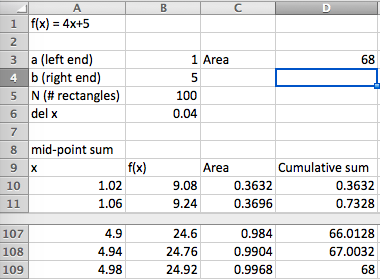
\includegraphics[width=\linewidth]{images/sec7-2-sol1a.png}
\end{sbspanel}%
\end{sidebyside}%
\end{enumerate}
\end{divisionexercise}%
\begin{divisionexercise}{2}{}{}{g:exercise:idm291741518704}%
Let \(f(x) = 6 x^2 + 3\).  We are told that \(F(x) = 2 x^3 + 3 x - 2\) is an anti-derivative.%
%
\begin{enumerate}[label=(\alph*)]
\item{}Verify that \(f(x)\) is a derivative of \(F(x)\).%
\item{}Use the fundamental theorem of calculus to evaluate \(\int_{-2}^4 f(x)\  dx\).%
\item{}Approximate \(\int_{-2}^4 f(x)\ dx\), using Riemann sums and 100 intervals.%
\end{enumerate}
\end{divisionexercise}%
\begin{divisionexercise}{3}{}{}{g:exercise:idm291741512912}%
Let \(f(x) = 5/x\).  We are told that \(F(x) = \ln(x^5) + 9\) is an anti-derivative.%
%
\begin{enumerate}[label=(\alph*)]
\item{}Verify that \(f(x)\) is a derivative of \(F(x)\).%
\item{}Use the fundamental theorem of calculus to evaluate \(\int_1^{20} f(x)\ dx\).%
\item{}Approximate \(\int_1^{20} f(x)\ dx\), using Riemann sums and 200 intervals.%
\end{enumerate}
\par\smallskip%
\noindent\textbf{Solution}.\hypertarget{g:solution:idm291741507280}{}\quad{}%
\begin{enumerate}[label=(\alph*)]
\item{}%
\begin{equation*}
F' (x)=\frac{d}{dx} [\ln(x^5 )+ 9]=\frac{1}{x^5}   (5x^4 )+ 0=\frac{5}{x}
\end{equation*}
or%
%
\begin{equation*}
F' (x)=\frac{d}{dx} [\ln(x^5 )+ 9]=\frac{d}{dx} [5\ln(x)+ 9]=5\frac{1}{x}+ 0=\frac{5}{x}
\end{equation*}
\item{}%
\begin{equation*}
\int_1^{20}\frac{5}{x} dx=F(20)-F(1)=\ln(20^5 )+9-(\ln(1)+9)=ln(20^5) =14.98
\end{equation*}
%
\item{}The midpoint sum with N = 200 gives an approximation of 14.978%
\begin{sidebyside}{1}{0.25}{0.25}{0}%
\begin{sbspanel}{0.5}%
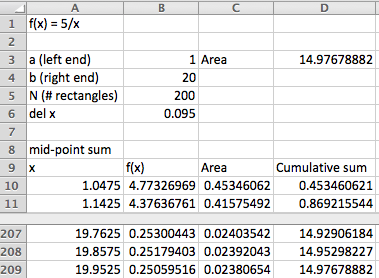
\includegraphics[width=\linewidth]{images/sec7-2-sol3a.png}
\end{sbspanel}%
\end{sidebyside}%
\end{enumerate}
\end{divisionexercise}%
\begin{divisionexercise}{4}{}{}{g:exercise:idm291741501600}%
Let \(f(x) = (2 x +3)^4\).  We are told that \(F(x) = 0.1 (2 x + 3)^5\) is an anti-derivative.%
%
\begin{enumerate}[label=(\alph*)]
\item{}Verify that \(f(x)\) is a derivative of \(F(x)\).%
\item{}Use the fundamental theorem of calculus to evaluate \(\int_{-1}^1 f(x)\ dx\).%
\item{}Approximate \(\int_{-1}^1 f(x)\ dx,\) using Riemann sums and 100 intervals.%
\end{enumerate}
\end{divisionexercise}%
\begin{divisionexercise}{5}{}{}{g:exercise:idm291741495808}%
Let \(f(x) = x exp(-0.05 x)\).  We are told that \(F(x) = -20 (x+20) \exp(-0.05x)+3\) is an anti-derivative.%
%
\begin{enumerate}[label=(\alph*)]
\item{}Verify that \(f(x)\) is a derivative of \(F(x)\).%
\item{}Use the fundamental theorem of calculus to evaluate \(\int_0^{10} f(x)\ dx\).%
\item{}Approximate \(\int_0^{10} f(x)\ dx\), using Riemann sums and 100 intervals.%
\end{enumerate}
\par\smallskip%
\noindent\textbf{Solution}.\hypertarget{g:solution:idm291741490144}{}\quad{}%
\begin{enumerate}[label=(\alph*)]
\item{}%
\begin{equation*}
F'(x)=\frac{d}{dx}  [-20(x+20)  e^{-0.05x}+3]
\end{equation*}
%
\begin{equation*}
=-20 [(1)  e^{-0.05x}+(x+20)  e^{-0.05x} (-0.05)] 
\end{equation*}
%
\begin{equation*}
= [(-20)  e^{-0.05x}+(x+20)  e^{-0.05x}]    
\end{equation*}
%
\begin{equation*}
=e^{-0.05x}  [(-20)+(x+20)] 
\end{equation*}
%
\begin{equation*}
=e^{-0.05x} x 
\end{equation*}
%
\item{}%
\begin{equation*}
\int_0^{10}x e^{-0.05 x} dx=F(10)-F(0)=-360.92-(-397)=36.08>
\end{equation*}
%
\item{}The midpoint sum with N = 100 gives an approximation of 38.06%
\begin{sidebyside}{1}{0.25}{0.25}{0}%
\begin{sbspanel}{0.5}%
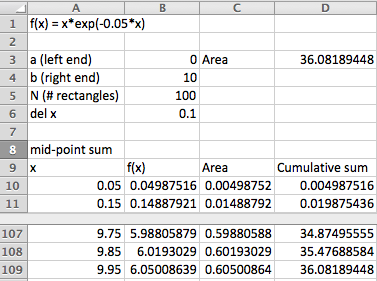
\includegraphics[width=\linewidth]{images/sec7-2-sol5a.png}
\end{sbspanel}%
\end{sidebyside}%
\end{enumerate}
\end{divisionexercise}%
\begin{divisionexercise}{6}{}{}{g:exercise:idm291741483376}%
Explain why, if \(F(x)\) is an anti-derivative of \(f(x)\), then \(F(x) + 7\) is also an anti-derivative of \(f(x)\).%
\end{divisionexercise}%
\begin{divisionexercise}{7}{}{}{g:exercise:idm291741480992}%
Using an area function from Riemann sums and best fitting curves we have guessed that a quadratic function will have a cubic anti-derivative.%
%
\begin{enumerate}[label=(\alph*)]
\item{}Find an anti-derivative of \(f(x)=-x^2+6x-2\)%
\item{}Use the fundamental theorem of calculus to evaluate%
\begin{itemize}[label=\textbullet]
\item{}\(\displaystyle \int_0^3 f(x)\ dx\)%
\item{}\(\displaystyle \int_{-2}^4 (x)\ dx\)%
\end{itemize}
.%
\end{enumerate}
\par\smallskip%
\noindent\textbf{Solution}.\hypertarget{g:solution:idm291741476576}{}\quad{}%
\begin{enumerate}[label=(\alph*)]
\item{}The anti-derivative should be a cubic, so something of the form%
%
\begin{equation*}
F(x)=ax^3+bx^2+cx+d
\end{equation*}
And the derivative should be \(f(x)= -x^2+6x-2\).%
\par
We can '{}'{}guess and check'{}'{}: \(F(x)=-1/3 x^3+3x^2-2x+0\) and sure enough, the derivative is \(f(x)\).%
\par
If you are not comforsidebyside with that method note that%
%
\begin{equation*}
F' (x)=3ax^2+2bx+c
\end{equation*}
So \(3a= -1\),\(2b=6\), and \(c=-2\).%
\par
Hence \(a= -1/3\),   \(b=3\), and \(c=-2\).%
\par
There are no conditions on \(d\), so that coefficient can be anything. We picked 0 to keep things simple. But then%
%
\begin{equation*}
F(x)=ax^3+bx^2+cx+d=-1/3 x^3+3x^2-2x
\end{equation*}
\item{}Use the fundamental theorem of calculus to evaluate%
\begin{itemize}[label=\textbullet]
\item{}%
\begin{equation*}
\int_0^3 f(x)\ dx=F(3)-F(0)=(-9+27-6)-(0)= 12
\end{equation*}
%
\item{}%
\begin{equation*}
\int_{-2}^4 (x)\ dx=F(4)-F(-2)
\end{equation*}
%
\begin{equation*}
=(-64/3+48-8)-(8/3+12+4)= -24+40-16=0
\end{equation*}
%
\end{itemize}
.%
\end{enumerate}
\end{divisionexercise}%
\begin{divisionexercise}{8}{}{}{g:exercise:idm291741464112}%
Using an area function from Riemann sums and best fitting curves we have guessed that a cubic function will have a fourth degree anti-derivative.%
%
\begin{enumerate}[label=(\alph*)]
\item{}Find an anti-derivative of \(f(x)=x^3+9x^2+7x-3\).%
\item{}Use the fundamental theorem of calculus to evaluate \(\int_1^5 f(x)\ dx\).%
\end{enumerate}
\end{divisionexercise}%
\begin{divisionexercise}{9}{}{}{g:exercise:idm291741460480}%
I am interested in finding an anti-derivative for \(f(x)=e^{2x}\).%
%
\begin{enumerate}[label=(\alph*)]
\item{}Using Excel and 100 subintervals of \(0 \le  x \le  2\), compute an approximate area function for \(f(x)\).  Find a best fitting curve that fits the data well.  (It may help to use a secondary axis for the area data.)%
\item{}Based on your best fitting curve, use guess and check to find the anti-derivative.%
\end{enumerate}
\par\smallskip%
\noindent\textbf{Solution}.\hypertarget{g:solution:idm291741456528}{}\quad{}%
\begin{enumerate}[label=(\alph*)]
\item{}A quick computation gives the total area:%
\begin{sidebyside}{1}{0}{0}{0}%
\begin{sbspanel}{1}%
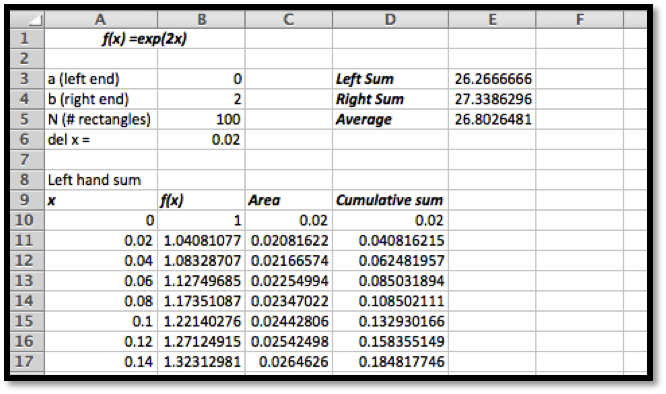
\includegraphics[width=\linewidth]{images/sec7-2-sol9a.png}
\end{sbspanel}%
\end{sidebyside}%
\par
The area under the curve is approx. 26.8.%
\par
The area under the curve looks like an exponential curve.%
\par
A curve fitting using the Trendlines gives us that%
%
\begin{equation*}
F(x)= 0.1618 e^2.739x
\end{equation*}
Note that this is not a very good approximation. The curve does not follow the data very well on the right hand side of the graph.%
\item{}Based on the curve we would say that the anti-derivative should be an exponential function. The derivative of \(e^{2x}\) is \(2e^{2x}\), so it seems reasonable to start with the anti-derivative being \(F(x)=A e^{2x}+B\).%
\par
Then the derivative has to  be \(f(x)\).%
%
\begin{equation*}
F' (x)=A e^2x  (2)+0=2A e^2x+0=e^2x
\end{equation*}
Hence A=0.5 and we may choose B to be any constant we want. Then%
%
\begin{equation*}
F(x)=1/2  e^2x+B  
\end{equation*}
That shows us where the problem is in our estimate.  Excel’s best fitting routine does not allow for constants in exponential functions.  Since \(F(0)=.5+B\), and \(Area(0)=0\), we need to add .5 to the area to get a good best fit curve.  Then the best fit line works.%
\begin{sidebyside}{1}{0}{0}{0}%
\begin{sbspanel}{1}%
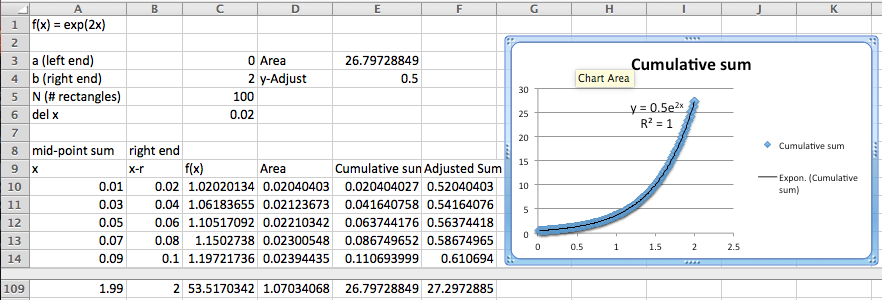
\includegraphics[width=\linewidth]{images/sec7-2-sol9b.png}
\end{sbspanel}%
\end{sidebyside}%
\end{enumerate}
\end{divisionexercise}%
\begin{divisionexercise}{10}{}{}{g:exercise:idm291741443408}%
I am interested in finding an anti-derivative for \(f(x)=e^{-5x}\).%
%
\begin{enumerate}[label=(\alph*)]
\item{}Using Excel and 100 subintervals of \(0 \le  x \le  2\), compute an approximate area function for \(f(x)\).  Find a best fitting curve that fits the data well.  (It may help to use a secondary axis for the area data.)%
\item{}Based on your best fitting curve, use guess and check to find the anti-derivative.%
\end{enumerate}
\end{divisionexercise}%
\begin{divisionexercise}{11}{}{}{g:exercise:idm291741439312}%
I am interested in finding an anti-derivative for \(f(x)=1/x\).%
%
\begin{enumerate}[label=(\alph*)]
\item{}Using Excel and 100 subintervals of \(1 \le  x \le  5\), compute an approximate area function for \(f(x)\).  Find a best fitting curve that fits the data well.  (It may help to use a secondary axis for the area data.)%
\item{}Based on your best fitting curve, use guess and check to find the anti-derivative.%
\end{enumerate}
\par\smallskip%
\noindent\textbf{Solution}.\hypertarget{g:solution:idm291741435360}{}\quad{}%
\begin{enumerate}[label=(\alph*)]
\item{}\begin{sidebyside}{1}{0}{0}{0}%
\begin{sbspanel}{1}%
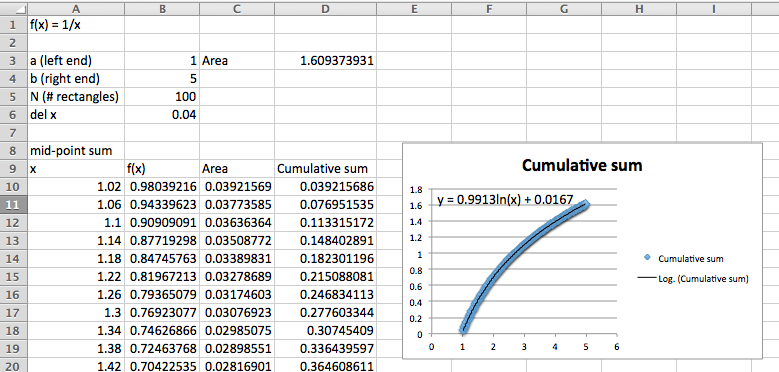
\includegraphics[width=\linewidth]{images/sec7-2-sol11a.png}
\end{sbspanel}%
\end{sidebyside}%
\par
The cumulative function looks like a logarithmic function.%
\par
The Trendline approximation gives the equation \(y = 0.9913ln(x) + 0.0167\).%
\par
We can make the fit better when we realize that we are evaluating at the midpoint of each interval but taking the are to the end of the interval.  We want to look at an adjusted x at the right side of each interval.%
\begin{sidebyside}{1}{0}{0}{0}%
\begin{sbspanel}{1}%
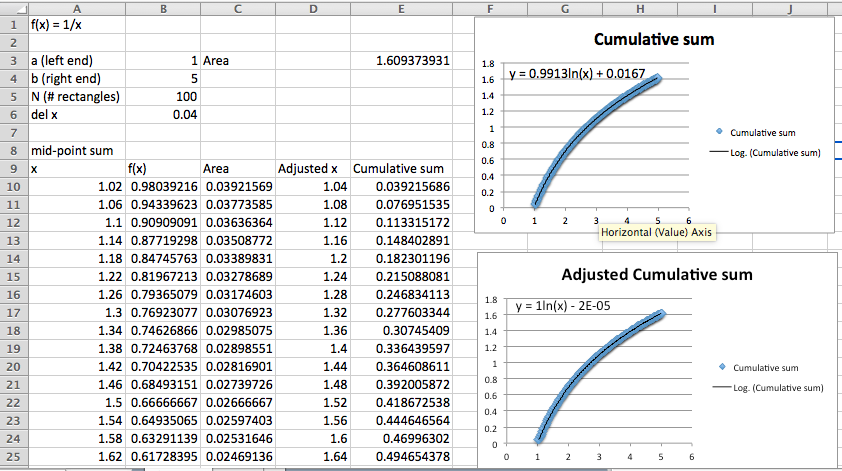
\includegraphics[width=\linewidth]{images/sec7-2-sol11b.png}
\end{sbspanel}%
\end{sidebyside}%
\par
Rounding off the coefficients, we would have that%
%
\begin{equation*}
F(x) = ln(x) 
\end{equation*}
\item{}We would say that the anti-derivative is \(F(x)=\ln(x)+constant\).%
\par
And we have seen before that%
%
\begin{equation*}
F'(x)=\frac{d}{dx}  \ln(x)+\frac{d}{dx} constant=\frac{1}{x}
\end{equation*}
\end{enumerate}
\end{divisionexercise}%
\end{exercises-subsection}
\end{sectionptx}
%
%
\typeout{************************************************}
\typeout{Section 1.3 Basic Antidifferentiation}
\typeout{************************************************}
%
\begin{sectionptx}{Basic Antidifferentiation}{}{Basic Antidifferentiation}{}{}{x:section:sec-7-3-BasicAntidifferentiation}
In the last section we looked at the fundamental theorem of calculus and saw that it could be used to find definite integrals.  We saw%
\begin{assemblage}{}{g:assemblage:idm291741423824}%
\terminology{Fundamental Theorem of Calculus (second version)} Let \(f(x)\) be a continuous function on the interval \([a, b]\).  Suppose \(F(x)\) is any continuous,  differentiable function with \(\frac{d}{dx} F(x)=f(x)\).  Then \(\int_a^b f(t)\ dt=F(b)-F(a)\).%
\end{assemblage}
We thus find it very useful to be able to systematically find an anti-derivative of a function.  The standard notation is to use an integral sign without the limits of integration to denote the general anti-derivative. Thus \(\int_a^b f(t)dt\) is referred to as the definite integral of \(f(x)\) from \(a\) to \(b\),  and is a number.  In contrast, \(\int f(x) dx\) is the indefinite integral of \(f(x)\) and it is a function.  We use indefinite integrals or anti-derivatives to evaluate definite integrals or areas.%
\par
We find anti-derivatives by starting with the differentiation formulas of basic functions and manipulating them so the derivative is a nice function%
\par
\terminology{Elementary Anti-derivative 1} – Find a formula for \(\int x^n\  dx\). We start with the closest differentiation formula \(\frac{d}{dx} x^n=nx^{n-1}\), and manipulate it so \(x^n\) is on the right hand side.  We first replace \(n\) with \(n+1\) to get \(\frac{d}{dx}  x^{n+1}=(n+1)x^n\).  We then divide both sides by \(n+1\) to obtain \(x^n=\frac{d}{dx}   x^{n+1}/(n+1)\).  Finally, we note that adding a constant \(C\) does not change the derivative, so  \(x^n=\frac{d}{dx}  (x^{n+1}/(n+1)+C)\).  Since we have divided by \(n+1\), we need to insist that \(n+1\ne 0\).  Using the notation of indefinite integrals we obtain our power rule formula:%
\begin{assemblage}{}{g:assemblage:idm291741410688}%
%
\begin{equation*}
\int x^n\  dx=\frac{x^{n+1}}{n+1}+C, \hbox{assuming }n\ne -1.
\end{equation*}
%
\end{assemblage}
Note that this matches the pattern we found in the last section.%
\par
\terminology{Elementary Anti-derivative 2} – Find a formula for \(\int 1/x \ dx\). We start with the closest differentiation formula \(\frac{d}{dx}   \ln (x)=1/x\).  In this case we need to note that natural logarithms are only defined positive numbers and we would like a formula that is true for positive and negative numbers.  We can do this with an appropriate use of absolute value bars.  Thus \(\frac{d}{dx} (\ln(|x|)+C)=1/x\), and we have our second formula:%
\begin{assemblage}{}{g:assemblage:idm291741407040}%
%
\begin{equation*}
\int 1/x\  dx=\ln |x|+C.
\end{equation*}
%
\end{assemblage}
\terminology{Elementary Anti-derivative 3} – Find a formula for \(\int e^x\  dx\). Once again, we start with the closest differentiation formula \(\frac{d}{dx}  e^x=e^x\). In this case we don't have to do any manipulation, and we have our formula:%
\begin{assemblage}{}{g:assemblage:idm291741404512}%
%
\begin{equation*}
\int e^x \ dx=e^x+C.
\end{equation*}
%
\end{assemblage}
\terminology{Elementary Anti-derivative 4} – Find a formula for \(\int a^x\  dx\) for a positive number a. This formula requires a bit more work.  We start with the formula \(\frac{d}{dx}  a^x=\ln (a) a^x\).   Dividing both sides by the constant ln(a) gives \(a^x=\frac{d}{dx}  (a^x/\ln (a) +C)\)  Thus our integral is:%
\begin{assemblage}{}{g:assemblage:idm291741401664}%
%
\begin{equation*}
\int a^x  dx=\frac{a^x}{\ln (a)} +C.
\end{equation*}
%
\end{assemblage}
\terminology{Sum, Difference, and Constant Multiple rules} – The rules we had for taking derivatives of sums, differences, and constant multiples of functions translate into similar rules for integrals.%
\par
The derivatives of a sum rule, \(\frac{d}{dx}(f(x)+g(x))=\frac{d}{dx}f(x)+\frac{d}{dx}g(x)\), becomes the%
\begin{assemblage}{}{g:assemblage:idm291741399184}%
\terminology{Integral of a Sum Rule}:%
\par
%
\begin{equation*}
\int (f(x)+g(x))\ dx=\int f(x)\ dx+\int g(x)\ dx
\end{equation*}
%
\end{assemblage}
The derivatives of a difference rule, \(\frac{d}{dx}(f(x)-g(x))=\frac{d}{dx}f(x)-\frac{d}{dx}g(x)\), becomes the%
\begin{assemblage}{}{g:assemblage:idm291741396848}%
\terminology{Integral of a Difference Rule}:%
\par
%
\begin{equation*}
\int (f(x)-g(x))\ dx=\int f(x)\ dx-\int g(x)\ dx
\end{equation*}
%
\end{assemblage}
\begin{assemblage}{}{g:assemblage:idm291741395424}%
\terminology{Integral of a Constant Multiple Rule}:%
\par
%
\begin{equation*}
\int cf(x) dx=c\int f(x)\ dx
\end{equation*}
%
\end{assemblage}
We can use these rules to find the indefinite integrals on a lot of functions.  They cover all polynomials.%
\begin{example}{Antiderivative of integral powers.}{g:example:idm291741393360}%
Find the integral \(\int 3x^5+4x^2+5+\frac{7}{x}\ dx\).%
\par
\terminology{Solution}%
%
\begin{equation*}
\int 3x^5+4x^2+5+\frac{7}{x}\ dx
\end{equation*}
%
\begin{equation*}
=\int 3x^5\ dx+\int 4x^2\ dx+\int 5\ dx+\int \frac{7}{x}\ dx\qquad\hbox{(sum rule)}
\end{equation*}
%
\begin{equation*}
=3\int x^5\ dx+4\int x^2\ dx+5\int \ dx+\int 7\frac{1}{x}\ dx\qquad\hbox{(constant multiple rule)}
\end{equation*}
%
\begin{equation*}
=3\int x^5\ dx+4\int x^2\ dx+5\int \ dx+ 7\ln|x|+C\qquad\hbox{(natural log rule)}
\end{equation*}
%
\begin{equation*}
=\frac{3}{6} x^6+\frac{4}{3}x^3+5x+ 7\ln|x|+C\qquad\hbox{(power rule)}
\end{equation*}
One might argue that the last line should have been%
%
\begin{equation*}
=\frac{3}{6} x^6+C_1+\frac{4}{3}x^3+C_2+5x+C_3+ 7\ln|x|+C_4
\end{equation*}
since each indefinite integral gets a constant C.  However all of the \(C_i\)’s used here are arbitrary constants and they can be collapsed together into a single constant C.%
\end{example}
We can also use these rules to find indefinite integrals for roots.%
\begin{example}{Antiderivative of fractional powers.}{g:example:idm291741386384}%
Find the integral \(\int \sqrt{2x}+\sqrt[3]{4x}\ dx\).%
\par
Solution%
%
\begin{equation*}
\int \sqrt{2x}+\sqrt[3]{4x}\ dx
=\int \sqrt{2x}\ dx+\int \sqrt[3]{4x}\ dx\qquad\hbox{(sum rule)}
\end{equation*}
%
\begin{equation*}
=\sqrt{2}\int \sqrt{x}\ dx+\sqrt[3]{4}\int \sqrt[3]{x}\ dx \qquad\hbox{(constant multiple rule)}
\end{equation*}
%
\begin{equation*}
=\sqrt{2}\int x^{(1/2)}\ dx+\sqrt[3]{4}\int x^{(1/3)}\ dx\qquad\hbox{(rules of exponents)}
\end{equation*}
%
\begin{equation*}
=\sqrt{2} x^{(3/2)}(2/3)+\sqrt[3]{4}x^{(4/3)}(3/4)+C\qquad\hbox{(power rule)}
\end{equation*}
\end{example}
We can also find anti-derivatives of exponential and power functions.%
\begin{example}{Antiderivative of power and exponential functions.}{g:example:idm291741381904}%
Find the integral \(\int 2*3^x+4e^x\ dx\).%
\par
Solution%
%
\begin{equation*}
\int 2*3^x+4e^x\ dx=\int 2*3^x\ dx+\int 4e^x\ dx\qquad\hbox{(sum rule)}
\end{equation*}
%
\begin{equation*}
=2\int 3^x\ dx+4\int e^x\ dx\qquad\hbox{(constant multiple rule)}
\end{equation*}
%
\begin{equation*}
=\frac{2}{\ln(3)} 3^x+4 e^x+C\qquad\hbox{(exponential rules)}
\end{equation*}
\end{example}
As we mentioned earlier in the section, the normal reason for wanting to find indefinite integrals is to be able to use them with the fundamental theorem of calculus to find definite integrals.%
\begin{example}{Area under a polynomial function.}{g:example:idm291741377856}%
Evaluate the definite integral \(\int_1^3 6x^2+2\ dx\).%
\par
Solution%
\par
We first evaluate the indefinite integral to find an anti-derivative.%
%
\begin{equation*}
\int 6x^2+2\ dx=2x^3+2x+C.
\end{equation*}
Since we can use any anti-derivative, we simplify by setting \(C = 0\) and choosing the anti-derivative  \(F(x)=2x^3+2x\).%
%
\begin{equation*}
\int_1^3 6x^2+2\ dx=F(3)-F(1)=60-4=56.
\end{equation*}
\end{example}
\begin{example}{Area under \(\frac{1}{x}\).}{g:example:idm291741373168}%
Evaluate the definite integral \(\int_1^{100}\frac{1}{x} dx\).%
\par
Solution%
\par
We first evaluate the indefinite integral to find an antiderivative.%
%
\begin{equation*}
\int \frac{1}{x}\ dx=\ln(|x|)+C
\end{equation*}
Since we can use any antiderivative, we simplify by setting \(C = 0\) and choosing that anti-derivative  \(F(x)=\ln(|x|)\).%
%
\begin{equation*}
\int_1^{100}\frac{1}{x}\ dx=F(100)-F(1)=\ln(100)-\ln(1)=\ln(100).
\end{equation*}
\end{example}
\begin{example}{Using the FTC when the function is fit from data.}{g:example:idm291741368208}%
From experience, I know that the output of an oil well follows a model of exponential decay.  I have the following data for the production, in barrels, for the first 5 months.%
\begin{sidebyside}{1}{0}{0}{0}%
\begin{sbspanel}{1}%
{\centering%
{\tabularfont%
\begin{tabular}{cccccc}\hrulethick
Month&Jan&Feb&Mar&Apr&May\tabularnewline\hrulethin
Production&1000&971&925&887&859\tabularnewline\hrulemedium
\end{tabular}
}%
\par}
\end{sbspanel}%
\end{sidebyside}%
\par
Find the production over the first 5 years.%
\par
Solution%
\par
The total production for 5 years will be the definite integral of the production function for the first 60 months.  We first use Excel to find a best fitting exponential function.%
\begin{sidebyside}{1}{0.1}{0.1}{0}%
\begin{sbspanel}{0.8}%
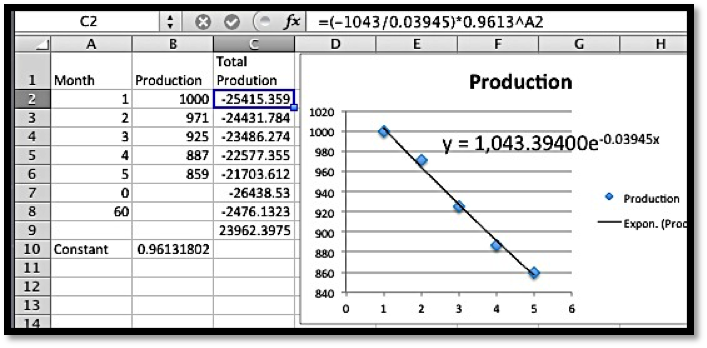
\includegraphics[width=\linewidth]{images/sec7-3-1.png}
\end{sbspanel}%
\end{sidebyside}%
\par
The production function (P) in terms of the number of months (x) is given by%
%
\begin{equation*}
P(x)=1043 e^{-0.03945 x}
\end{equation*}
We would like to take an anti-derivative, but we don’t have a formula for this anti-derivative yet.  However, we note%
%
\begin{equation*}
e^{-0.03945 x}=  (e^{-0.03945} )^x=0.9613^x
\end{equation*}
and we know that \(\ln (0.9613)=-0.03945\). We can now use our exponential rule, and%
%
\begin{equation*}
AntiderivP(x)=\frac{(1043*0.9613^x)}{(-0.03945)}+C
\end{equation*}
Since we can use any anti-derivative, we simplify by setting \(C = 0\). We can do this without creating any problems because we are using the equation where two values of the anti-derivative will be subtracted from one another, and hence the C values would cancel anyways. We now evaluate our integral.%
%
\begin{equation*}
TotalP(60)= ArtiderivP(60)– AntiderivP(0)
\end{equation*}
%
\begin{equation*}
= (-2467) – (-26438) = 23962
\end{equation*}
Thus over 5 years the well will produce 23,962 barrels.%
\end{example}
Another application for anti-derivatives is solving an initial value problem.  In that case we want to a particular anti-derivative that has a particular value for a specified x. In this situation we may not set C to zero. In fact, part of the problem will be to find the appropriate value of C.%
\begin{example}{Finding a value of C to match initial conditions.}{g:example:idm291741351088}%
The marginal cost (MC) of producing a certain quantity (q) of widgets is given by%
%
\begin{equation*}
MC(q)=5-0.002 q
\end{equation*}
The cost of producing 1000 widgets is \textdollar{}6,000.  Assume that the derivative of the cost function is approximated closely enough by the marginal cost to be used interchangeably.  Find a cost function for producing widgets.%
\par
\terminology{Solution}: Since Cost is an anti-derivative of the Marginal Cost we have \(Cost(q) = 5q - 0.001*q^2  + C\)%
\par
We also know \(Cost(1000) = 6000\).  Plugging that in gives%
%
\begin{equation*}
Cost(1000)= 5*1000 - 0.001*1000^2  + C=6000
\end{equation*}
Solving for C gives \(C = 2000\).  Thus our cost function is%
%
\begin{equation*}
Cost(q) = 5q - 0.001*q^2  + 2000
\end{equation*}
\end{example}
\begin{example}{Building a profit function form data.}{g:example:idm291741345152}%
Experience tells me that the marginal profit of producing gadgets is a linear function.  My start-up costs are \textdollar{}2 million.  I have the following data with my units being thousands of dollars per millions of units.%
\begin{sidebyside}{1}{0}{0}{0}%
\begin{sbspanel}{1}%
{\centering%
{\tabularfont%
\begin{tabular}{cccccc}\hrulethick
Production&0&1&2&3&4\tabularnewline\hrulethin
Marginal Profit&\textdollar{}3,3967&\textdollar{}3,603&\textdollar{}3,236&\textdollar{}2,795&\textdollar{}2,384\tabularnewline\hrulemedium
\end{tabular}
}%
\par}
\end{sbspanel}%
\end{sidebyside}%
\par
Produce a profit function, find the number of units that maximizes profit, and find the maximum profit%
\par
Solution%
\par
I start by finding a best fitting line to the data.%
\begin{sidebyside}{1}{0.1}{0.1}{0}%
\begin{sbspanel}{0.8}%
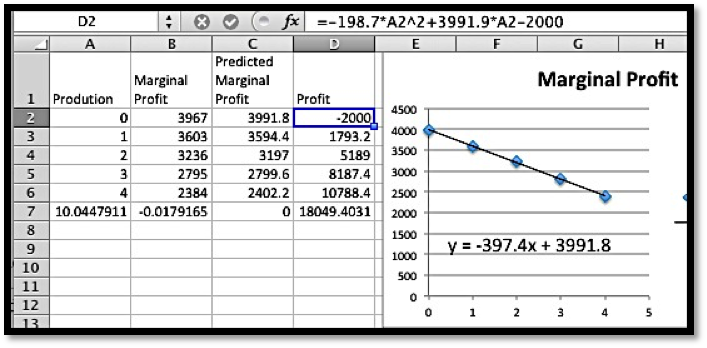
\includegraphics[width=\linewidth]{images/sec7-3-2.png}
\end{sbspanel}%
\end{sidebyside}%
\par
Excel tells me the marginal profit function is%
%
\begin{equation*}
MP(x) = -397.4 x + 3991.8
\end{equation*}
We have maximum profit when the marginal profit is zero.  Using Goal Seek, the Marginal Profit is zero with a production of 10.0448 millions of units.  The anti-derivative of this function is%
%
\begin{equation*}
P(x)= -198.7 x^2  + 3991.8x + C
\end{equation*}
Plugging in the initial costs into the production model, recalling that our function is written in thousands of dollars per millions of widgets, gives%
%
\begin{equation*}
P(0) = -2000 = C
\end{equation*}
So our profit function is%
%
\begin{equation*}
P(x)= -198.7 x^2  + 3991.8 x-2000
\end{equation*}
We saw that \(MP(x) = 0\), when \(x = 10.0448\). The maximum profit is the computed by evaluating \(P(x)\) at \(x = 10.0448\). A quick computation shows that the  maximum profit is \textdollar{}18,049 thousands of dollars, or a bit more than \textdollar{}18 million.%
\end{example}
\begin{assemblage}{}{g:assemblage:idm291741328432}%
It is worthwhile summarizing our list of integration formulas.%
\begin{sidebyside}{1}{0}{0}{0}%
\begin{sbspanel}{1}%
{\centering%
{\tabularfont%
\begin{tabular}{cc}\hrulethick
\(f(x)\)&\(\int f(x)\ dx\)\tabularnewline\hrulethin
\(\displaystyle x^n\hbox{, assuming }n\ne 1\)&\(\displaystyle \frac{x^{n+1}}{n+1}+C\)\tabularnewline\hrulemedium
\(\displaystyle \frac{1}{x}\)&\(\displaystyle \ln|x|+C\)\tabularnewline\hrulemedium
\(\displaystyle e^x\)&\(\displaystyle e^x+C\)\tabularnewline\hrulemedium
\(\displaystyle a^x\)&\(\displaystyle \frac{a^x}{\ln(a)}+C\)\tabularnewline\hrulemedium
\(\displaystyle (f+g)(x)\)&\(\displaystyle \int f(x)dx+\int g(x)dx\)\tabularnewline\hrulemedium
\(\displaystyle (f-g)(x)\)&\(\displaystyle \int f(x)dx-\int g(x)dx\)\tabularnewline\hrulemedium
\(\displaystyle c*f(x)\)&\(\displaystyle c*\int f(x)dx\)\tabularnewline\hrulemedium
\end{tabular}
}%
\par}
\end{sbspanel}%
\end{sidebyside}%
\end{assemblage}
A word of warning – The anti-differentiation formulas we have produced only work for the functions given, allowing for changes in variables.  At this point the only way we have for finding  \(\int(3x+5)^2 dx\) is expand the integrand getting  \(\int(9x^2+30x+25)dx\) before applying our rules.  In general the process of finding anti-derivatives symbolically is an art form that we only begin to work with in this course.%
%
%
\typeout{************************************************}
\typeout{Exercises 1.3.1 Exercises: Basic Antidifferentiation Problems}
\typeout{************************************************}
%
\begin{exercises-subsection}{Exercises: Basic Antidifferentiation Problems}{}{Exercises: Basic Antidifferentiation Problems}{}{}{x:exercises:exercises-set-sec-7-3}
Find antiderivatives for the given functions.%
\begin{divisionexercise}{1}{}{}{g:exercise:idm291741309936}%
%
\begin{equation*}
f(x)=3x+5.
\end{equation*}
\par\smallskip%
\noindent\textbf{Solution}.\hypertarget{g:solution:idm291741309408}{}\quad{}%
\begin{equation*}
F(x)=\frac{3x^2}{2}+5x+Constant
\end{equation*}
\end{divisionexercise}%
\begin{divisionexercise}{2}{}{}{g:exercise:idm291741308688}%
%
\begin{equation*}
f(x)=5x^3+4x+3.
\end{equation*}
\end{divisionexercise}%
\begin{divisionexercise}{3}{}{}{g:exercise:idm291741308032}%
%
\begin{equation*}
f(x)=x^{3,124,567}+2x^{473}+327 x^{-2,786,534}.
\end{equation*}
\par\smallskip%
\noindent\textbf{Solution}.\hypertarget{g:solution:idm291741307456}{}\quad{}%
\begin{equation*}
F(x)=\frac{x^{3,124,568}}{3,124,568}+2 \frac{x^{474}}{474}+327 \frac{x^{-2,786,533}}{-2,786,533}+Constant
\end{equation*}
\end{divisionexercise}%
\begin{divisionexercise}{4}{}{}{g:exercise:idm291741306528}%
%
\begin{equation*}
f(x)=\sqrt{11x}+\frac{5}{x}.
\end{equation*}
\end{divisionexercise}%
\begin{divisionexercise}{5}{}{}{g:exercise:idm291741305840}%
%
\begin{equation*}
f(x)=e^x+\left(\frac{1}{2}\right)^x.
\end{equation*}
\par\smallskip%
\noindent\textbf{Solution}.\hypertarget{g:solution:idm291741305280}{}\quad{}%
\begin{equation*}
F(x)=e^x+\frac{\left(\frac{1}{2}\right)^x}{\ln\left(\frac{1}{2}\right)}+Constant
\end{equation*}
\end{divisionexercise}%
\begin{divisionexercise}{6}{}{}{g:exercise:idm291741304368}%
\(f(x)=\pi^x+\pi^\pi+x^\pi.\)\end{divisionexercise}%
Evaluate the definite integrals by first finding an antiderivative.%
\begin{divisionexercise}{7}{}{}{g:exercise:idm291741303200}%
%
\begin{equation*}
\int_0^5 x+7\  dx
\end{equation*}
\par\smallskip%
\noindent\textbf{Solution}.\hypertarget{g:solution:idm291741301744}{}\quad{}%
\begin{equation*}
\int_0^5 (x+7)dx=F(5)- F(0)=\frac{25}{2}+35-0=\frac{95}{2}
\end{equation*}
\end{divisionexercise}%
\begin{divisionexercise}{8}{}{}{g:exercise:idm291741301008}%
%
\begin{equation*}
\int_1^{10}\frac{1}{x}\  dx
\end{equation*}
\end{divisionexercise}%
\begin{divisionexercise}{9}{}{}{g:exercise:idm291741300320}%
%
\begin{equation*}
\int_2^{10} 3x+\frac{5}{x}\  dx
\end{equation*}
\par\smallskip%
\noindent\textbf{Solution}.\hypertarget{g:solution:idm291741299760}{}\quad{}The anti-derivative is: \(F(x)=(3x^2)/2+5 \ln|x|\)%
%
\begin{equation*}
\int_2^{10} 3x+\frac{5}{x}  dx =F(10)-F(2)
=\frac{300}{2}+5 \ln(10)-\left(\frac{12}{2}+5 \ln(2) \right)
\end{equation*}
%
\begin{equation*}
=150+5 \ln(10)-6-5 \ln(2)=144+5(\ln(10)-\ln(2) )
\end{equation*}
%
\begin{equation*}
= 144+5 \ln\left(\frac{10}{2}\right)=144+5 \ln(5)
\end{equation*}
\end{divisionexercise}%
\begin{divisionexercise}{10}{}{}{g:exercise:idm291741297040}%
%
\begin{equation*}
\int_1^{100}\left(\frac{1}{2}\right)^x\   dx.
\end{equation*}
\end{divisionexercise}%
\begin{divisionexercise}{11}{}{}{g:exercise:idm291741296336}%
%
\begin{equation*}
\int_{-10}^2 e^x+e \  dx
\end{equation*}
\par\smallskip%
\noindent\textbf{Solution}.\hypertarget{g:solution:idm291741295792}{}\quad{}The anti-derivative is: \(F(x)=e^x+e x\)%
%
\begin{equation*}
\int_{-10}^2 e^x+e  dx =F(2)-F(-10)=e^2+2e-(e^{-10}-10 e)
\end{equation*}
%
\begin{equation*}
= e^2-\frac{1}{e^{10}} -8 e
\end{equation*}
\end{divisionexercise}%
\begin{divisionexercise}{12}{}{}{g:exercise:idm291741293632}%
%
\begin{equation*}
\int_{-2}^5 x^{-2}+x^{-1} \  dx
\end{equation*}
\end{divisionexercise}%
Solve the Initial value problem.%
\begin{divisionexercise}{13}{}{}{g:exercise:idm291741292480}%
Let \(f(x)=4x+3\).  The function \(F(x)\) is an antiderivative, and \(F(0)=7\).%
\par\smallskip%
\noindent\textbf{Solution}.\hypertarget{g:solution:idm291741290672}{}\quad{}The anti-derivative is: \(F(x)=2x^2+3x+C\).%
\par
\(F(0)= 7\) implies that \(F(0)=0+C=7\), so \(C = 7\)%
\par
Then \(F(x)=2x^2+3x+7\).%
\end{divisionexercise}%
\begin{divisionexercise}{14}{}{}{g:exercise:idm291741287200}%
Let \(f(x)=3x^2-6x+5\).  The function \(F(x)\)  is an antiderivative, and \(F(3)=17\).%
\end{divisionexercise}%
\begin{divisionexercise}{15}{}{}{g:exercise:idm291741285248}%
Let \(f(x)=100(0.95)^x\).  The function \(F(x)\)  is an antiderivative, and \(F(5)=9\).%
\par\smallskip%
\noindent\textbf{Solution}.\hypertarget{g:solution:idm291741283424}{}\quad{}The anti-derivative is:%
%
\begin{equation*}
F(x)=\frac{100 (0.95)^x }{\ln(0.95)}   +C
\end{equation*}
\(F(5)= 9\) implies that%
%
\begin{equation*}
F(5)=\frac{100 (0.95^5 )}{\ln(0.95)} +C=9
\end{equation*}
%
\begin{equation*}
C=9-\frac{100 (0.95^5 )}{\ln(0.95)}\approx 9+1508.54=1517.54
\end{equation*}
Then%
%
\begin{equation*}
F(x)\approx\frac{100 (0.95^x )}{\ln(0.95)} +1517.54
\end{equation*}
\end{divisionexercise}%
\begin{divisionexercise}{16}{}{}{g:exercise:idm291741279648}%
Let \(f(x)=7/x+x^2\).  The function \(F(x)\)  is an antiderivative, and \(F(1)=11\).%
\end{divisionexercise}%
\begin{divisionexercise}{17}{}{}{g:exercise:idm291741277696}%
An investment provides an income stream of \(1000 (0.95)^t\) dollars per year.  How much is received in the first 10 years?%
\par\smallskip%
\noindent\textbf{Solution}.\hypertarget{g:solution:idm291741276528}{}\quad{}%
\begin{equation*}
Income=\int_0^{10}1000(0.95)^t  dt
=\left.\frac{1000(0.95)^t)}{\ln(0.95)} \right|_{t=0}^{t=10}
\end{equation*}
%
\begin{equation*}
=\frac{1000(0.95)^{10}}{\ln(0.95)} -\frac{1000(0.95)^0)}{\ln(0.95)} 
\end{equation*}
%
\begin{equation*}
\approx -11672.81+19495.73=7822.91
\end{equation*}
\end{divisionexercise}%
\begin{divisionexercise}{18}{}{}{g:exercise:idm291741274688}%
A firm has a marginal profit function of \(MP(x) = 50 – 3 x\) in thousands of dollars per thousands of units.  How much is profit increased if production is shifted from 10 to 15 thousand units.%
\end{divisionexercise}%
\begin{divisionexercise}{19}{}{}{g:exercise:idm291741273424}%
After the first year, the rate of sales of a fad product are \(sales(t) = \frac{1000}{t}\) with time in years.  How many units are sold from the end of the first year to the end of the tenth year?%
\par\smallskip%
\noindent\textbf{Solution}.\hypertarget{g:solution:idm291741272320}{}\quad{}%
\begin{equation*}
sales=\int_1^{10}\frac{1000}{t} dt=1000 \ln(t) |_{t=1}^{t=10}
\end{equation*}
%
\begin{equation*}
=1000(\ln(10)-\ln(0) )
\end{equation*}
%
\begin{equation*}
=1000\ln(10)\approx 2302.58
\end{equation*}
\end{divisionexercise}%
\begin{divisionexercise}{20}{}{}{g:exercise:idm291741270576}%
A software company allows your company to expand the number of licenses your company owns by charging a marginal rate of \(MR(licenses)=\frac{200}{\sqrt{licenses}}\).  How much does it cost to increase your license from 1000 to 2000 licenses?%
\end{divisionexercise}%
\begin{divisionexercise}{21}{}{}{g:exercise:idm291741269280}%
The production function for a given oil well is \(rate(t) = 400(0.9)^t\) with time measured in years and production measured in millions of barrels of oil.%
%
\begin{enumerate}[label=(\alph*)]
\item{}How much oil is produced in the first year?%
\item{}How much oil is produced in the tenth year?%
\item{}If I need to produce 75 thousand barrels of oil per year for the well to be financially viable, what is the life of the well?%
\item{}How much oil will the well produce before being shut down?%
\end{enumerate}
\par\smallskip%
\noindent\textbf{Solution}.\hypertarget{g:solution:idm291741264992}{}\quad{}%
\begin{enumerate}[label=(\alph*)]
\item{}%
\begin{equation*}
Production=\int_0^{1}400(0.9)^t dt
=\left.\frac{400}{\ln(0.9)}  (0.9)^t \right|_{t=0}^{t=1}
\end{equation*}
%
\begin{equation*}
=\frac{400}{\ln(0.9)} (0.9-1)\approx 379.649
\end{equation*}
%
\item{}%
\begin{equation*}
Production=\int_9^{10}400(0.9)^t dt
=\left.\frac{400}{\ln(0.9)}  (0.9)^t \right|_{t=9}^{t=10}
\end{equation*}
%
\begin{equation*}
=\frac{400}{\ln(0.9)} (0.9^{10}-0.9^{9})\approx 147.08
\end{equation*}
%
\item{}%
\begin{equation*}
0.075=400*(0.9)^t
\end{equation*}
%
\begin{equation*}
t=ln(0.75/400)/ln(0.9)\approx 81.451
\end{equation*}
%
\item{}Use Goal seek.%
%
\begin{equation*}
75=400(0.9^t)
\end{equation*}
%
\begin{equation*}
t\approx 15.8881
\end{equation*}
\end{enumerate}
\end{divisionexercise}%
\begin{divisionexercise}{22}{}{}{g:exercise:idm291741259360}%
The expected value received from a particular revenue stream should be an exponential function.  I have the following data for income received over the past 5-year period.%
\begin{sidebyside}{1}{0}{0}{0}%
\begin{sbspanel}{1}%
{\centering%
{\tabularfont%
\begin{tabular}{cccccc}\hrulethick
Year&1&2&3&4&5\tabularnewline\hrulethin
Income&\textdollar{}1,030&\textdollar{}1,078&\textdollar{}1,110&\textdollar{}1,169&\textdollar{}1,225\tabularnewline\hrulemedium
\end{tabular}
}%
\par}
\end{sbspanel}%
\end{sidebyside}%
\par
How much do I expect to receive over the next 10 years?%
\end{divisionexercise}%
\begin{divisionexercise}{23}{}{}{g:exercise:idm291741251712}%
From experience, I expect the marginal revenue for my firm to be a quadratic function.  I have the following data on revenue at a variety of levels, with production in thousands of units and marginal profit in millions of dollars.%
\begin{sidebyside}{1}{0}{0}{0}%
\begin{sbspanel}{1}%
{\centering%
{\tabularfont%
\begin{tabular}{cccccc}\hrulethick
Production&\textdollar{}4.90&\textdollar{}7.04&9.00&11.03&14.00\tabularnewline\hrulethin
MProfit&7.40&9.12&9.90&9.89&8.40\tabularnewline\hrulemedium
\end{tabular}
}%
\par}
\end{sbspanel}%
\end{sidebyside}%
\par
What is the expected change in revenue as I increase production from 15 to 20 thousand units?%
\par\smallskip%
\noindent\textbf{Solution}.\hypertarget{g:solution:idm291741244112}{}\quad{}Using trend line, my function for \(MProfit\) is%
%
\begin{equation*}
MProfit=-0.01Production^2+2Production+0.11
\end{equation*}
Integrating from 15 to 20%
%
\begin{equation*}
Profit= \int_{15}^{20}-0.01x^2+2x+0.11  dx
\end{equation*}
%
\begin{equation*}
= \left.-\frac{0.01}{3} x^3+x^2+0.11x\right|_{x=15}^{x=20}
\approx 160.133
\end{equation*}
The profit is approximately \textdollar{}160.133 million.\end{divisionexercise}%
\end{exercises-subsection}
\end{sectionptx}
%
%
\typeout{************************************************}
\typeout{Section 1.4 Integration by Change of Variables or Substitution}
\typeout{************************************************}
%
\begin{sectionptx}{Integration by Change of Variables or Substitution}{}{Integration by Change of Variables or Substitution}{}{}{x:section:sec-7-4-ChangeVariables}
At the end of the last section we warned that the symbolic integration techniques we have developed only work for problems that exactly fit our formulas.  When we tried integrating an exponential function where the exponent was a constant times t, we had to change the base to get a function with only t in the exponent.  We want to develop one more technique of integration, that of change of variables or substitution, to handle integrals that are pretty close to our stated rules. This technique is often called u-substitution and is related to the chain rule for differentiation.%
\par
We start by exploring some examples where we can get the desired result by the guess and check technique.%
\begin{example}{Power of a linear by guess and check.}{x:example:power-of-linear}%
Find \(\int (3x+5)^7  dx\).%
\par
\terminology{Solution}:  We could do this problem by rewriting the integrand as an explicit seventh degree polynomial and then using the power and sum rules, but that is too much work.  Instead I will notice the integrand looks almost like a power, and thus guess an answer of \(\frac{1}{8} (3x+5)^8+C\).  I then check by differentiating.  Using the chain rule%
%
\begin{equation*}
\frac{d}{dx}  (\frac{1}{8} (3x+5)^8+C)=\frac{1}{8}*8(3x+5)^{8-1}*3=3(3x+5)^7.
\end{equation*}
. Thus our guess was off by a factor of 3 and the correct antiderivative is%
%
\begin{equation*}
\frac{1}{3}*1\frac{1}{8} (3x+5)^8+C=\frac{1}{24} (3x+5)^8+C.
\end{equation*}
\end{example}
We can easily use the same trick to produce a rule for powers of a linear polynomial.%
\begin{example}{Power of a generic linear by guess and check.}{g:example:idm291741232912}%
Find \(\int (ax+b)^n  dx\).%
\par
\terminology{Solution}:  As we did in example 1, we first guess the antiderivative to be \(\frac{1}{n+1} (ax+b)^{n+1}+C\). We then take the derivative of that expression and obtain \(a(ax+b)^n\).  This misses our integrand by a factor of \(a\).  We adjust by that factor and find the antiderivative is \(\frac{1}{a}  \frac{1}{n+1} (ax+b)^{n+1}+C\).%
\end{example}
We can easily use the same trick to produce a rule for functions that are the exponential of a linear function.%
\begin{example}{Antidifferentiation of an exponential function by guess and check.}{g:example:idm291741228240}%
Find \(\int e^{ax+b}  dx\).%
\par
\terminology{Solution}:  As we did in example 2, our first guess uses the basic rule without worrying about the linear term, so we guess \(e^{ax+b}+C\). We then take the derivative of that expression and obtain \(ae^{ax+b}\).  This misses our integrand by a factor of \(a\).  We adjust by that factor and find the antiderivative is \(\frac{1}{a} e^{ax+b}+C\).%
\end{example}
We run into a problem if we try to extend this method with quadratic terms.  If we start with \((x^2+5)^3\) and guess an antiderivative of \(\frac{1}{4} (x^2+5)^4\), when we differentiate we get \((x^2+5)^3 2x\) and are off by a factor of \(8x\).  However when we divide by that factor to get \(\frac{(x^2+5)^4}{8x}\) as a proposed antiderivative, and then differentiate again we get%
%
\begin{equation*}
\frac{4*2x(x^2+5)^3*8x-(x^2+5)^4*8}{8x}
\end{equation*}
which is not what we want.  The key is to start by recalling the chain rule%
%
\begin{equation*}
\frac{d}{dx}  (f(g(x)))=f'(g(x))g'(x).
\end{equation*}
We want to use the same rule with a different notation, using implicit differentiation and a new variable \(u\):%
%
\begin{equation*}
\frac{d}{dx}  (f(u))=f'(u)\frac{du}{dx}.
\end{equation*}
By the fundamental theorem of calculus, we can convert this to an integration formula:%
%
\begin{equation*}
\int f' (u)  \frac{du}{dx}  dx=f(u)+C.
\end{equation*}
We will generally simplify \(\frac{du}{dx} dx\) to \(du\), so our substitution rule is%
%
\begin{equation*}
\int f' (u)du=f(u)+C.
\end{equation*}
Let us rework some earlier examples with this method and then illustrate the method with a more difficult problem.%
\begin{example}{Power of linear example redone with change of variables.}{g:example:idm291741215296}%
Find \(\int (3x+5)^7 dx\).%
\par
\terminology{Solution}:  The obvious candidate for \(u\) is \(3x+5\).  Then \(du=3dx\).  Thus%
%
\begin{equation*}
\begin{aligned}  \int (3x+5)^7  dx
\amp =\frac{1}{3} \int (3x+5)^7  (3dx)
\amp \quad \hbox{ (Make u and du explicit.)}\\ 
\amp =\frac{1}{3} \int (u)^7  du
\amp \quad \hbox{ (Do the substitution.)}\\ 
\amp =\frac{1}{3*8} (u)^8+C
\amp \quad \hbox{ (Find the integral in terms of u.)}\\ 
\amp =\frac{1}{24} (3x+5)^8+C
\amp \quad \hbox{ (Substitute back.)}\\ 
\end{aligned}
\end{equation*}
\end{example}
This is easy to generalize for a power of a linear term.%
\begin{example}{Power of generic linear example redone with change of variables.}{g:example:idm291741210512}%
Find \(\int (ax+b)^n dx\).%
\par
\terminology{Solution}:  The obvious candidate for \(u\) is \(ax+b\).  Then \(du=a dx\).  Hence%
%
\begin{equation*}
\begin{aligned}  \int (ax+b)^n dx
\amp =\frac{1}{a} \int (ax+b)^n  (dx)
\amp \quad \hbox{ (Make u and du explicit.)}\\ 
\amp =\frac{1}{a} \int (u)^n  du
\amp \quad \hbox{ (Do the substitution.)}\\ 
\amp =\frac{1}{a*(n+1)} (u)^{n+1}+C
\amp \quad \hbox{ (Find the integral in terms of u.)}\\ 
\amp =\frac{1}{a*(n+1)} (ax+b)^{n+1}+C
\amp \quad \hbox{ (Substitute back.)}\\ 
\end{aligned}
\end{equation*}
\end{example}
To use this method with u replacing something more complicated than a linear term, we need to have \(du\) available, with the possible addition of multiplying by a scalar constant.%
\begin{example}{Power of quadratic function with change of variables.}{g:example:idm291741205184}%
Find \(\int (2x^3+11)^7 x^2 dx\).%
\par
\terminology{Solution}:  The obvious candidate for \(u\) is \(2x^3+11\).  Then \(du=6x^2d\)x.  Thus%
%
\begin{equation*}
\begin{aligned}  \int (2x^3+11)^7 x^2 dx
\amp =\frac{1}{6} \int (2x^3+11)^7 6x^2 dx)
\amp \quad \hbox{ (Make u and du explicit.)}\\ 
\amp =\frac{1}{6} \int (u)^7  du
\amp \quad \hbox{ (Do the substitution.)}\\ 
\amp =\frac{1}{6*8} (u)^8+C
\amp \quad \hbox{ (Find the integral in terms of u.)}\\ 
\amp =\frac{1}{48} (2x^3+11)^8+C
\amp \quad \hbox{ (Substitute back.)}\\ 
\end{aligned}
\end{equation*}
\end{example}
By convention, \(u\) is often used the new variable used with this change of variables technique, so the technique is often called u-substitution.%
\par
\terminology{Change of variables for definite integrals}%
\par
In the definite integral, we understand that a and b are the \(x\)-values of the ends of the integral.  We could be more explicit and write \(x=a\) and \(x=b\).  The last step in solving a definite integral is to substitute the endpoints back into the antiderivative we have found.  We can either change the variables for the endpoints as well, or we can convert the antiderivative back to the original variables before substituting.  Consider the following example.%
\begin{example}{A definite integral with change of variables.}{g:example:idm291741197264}%
Evaluate \(\int_1^3 e^{2x+5} dx\).%
\par
\terminology{Solution 1}:  (Convert everything to \(u\).) The obvious candidate for \(u\) is \(2x+5\).  Then    \(du=2dx\).  For the lower endpoint, \(x=1\) becomes \(u=7\).  For the upper endpoint \(x=3\) becomes \(u=11\).  Substituting,%
%
\begin{equation*}
\begin{aligned}  \int_1^3 e^{2x+5} dx
\amp =\frac{1}{2} \int_1^3 e^{2x+5} (2dx)
\amp \quad \hbox{ (Make u and du explicit.)}\\ 
\amp =\frac{1}{2} \int_{u=7}^{u=11}e^u du
\amp \quad \hbox{ (Do the substitution.)}\\ 
\amp =\left.\frac{1}{2} e^u\right|_7^{11}
\amp \quad \hbox{ (Find the antiderivative.)}\\ 
\amp =\frac{1}{2} e^{11}-\frac{1}{2} e^7.
\amp \quad \hbox{ (Evaluate.)}\\ 
\end{aligned}
\end{equation*}
\terminology{Solution 2}:  (Keeping, but labeling the endpoints.) We have the same u and du, but do not convert the endpoints.  To reduce confusion we make sure to label the variable when we are using both \(x\) and \(u\).  Thus,%
%
\begin{equation*}
\begin{aligned}  \int_1^3 e^{2x+5} dx
\amp =\frac{1}{2} \int_1^3 e^{2x+5} (2dx)
\amp \quad \hbox{ (Make u and du explicit.)}\\ 
\amp =\frac{1}{2} \int_{x=1}^{x=3}e^u du
\amp \quad \hbox{ (Do the substitution.)}\\ 
\amp =\left.\frac{1}{2} e^u\right|_{x=1}^{x=3}
\amp \quad \hbox{ (Find the antiderivative.)}\\ 
\amp =\left.\frac{1}{2} e^{2x+3}\right|_{x=1}^{x=3}
\amp \quad \hbox{ (Convert back.)}\\ 
\amp =\frac{1}{2}  e^{11}-\frac{1}{2} e^7.
\amp \quad \hbox{ (Evaluate.)}\\ 
\end{aligned}
\end{equation*}
\end{example}
It should be noted that when we change variables we may find ourselves looking at an integral from \(a\) to \(b\) where the \(b \lt a\).  We do not change the order of the endpoints.%
\begin{example}{A second definite integral with change of variables.}{g:example:idm291741186416}%
Evaluate \(\int_{-2}^1 x \exp(x^2)dx\)%
\par
\terminology{Solution}: (Convert everything to \(u\).) The obvious candidate for \(u\) is \(x^2\).  Then \(du=2x\  dx\). For the lower endpoint, \(x=-2\) becomes \(u=4\).  For the upper endpoint \(x=1\) becomes \(u=1\). Substituting,%
%
\begin{equation*}
\begin{aligned}  \int_{-2}^1 x e^{(x^2)}dx
\amp =\frac{1}{2} \int_{-2}^1 e^{(x^2)}(2x dx)
\amp \quad \hbox{ (Make u and du explicit.)}\\ 
\amp =\frac{1}{2} \int_{4}^{1}e^u du
\amp \quad \hbox{ (Do the substitution.)}\\ 
\amp =\left.\frac{1}{2} e^u\right|_4^{1}
\amp \quad \hbox{ (Find the antiderivative.)}\\ 
\amp =\frac{1}{2}  e^1-\frac{1}{2} e^4.
\amp \quad \hbox{ (Evaluate.)}\\ 
\end{aligned}
\end{equation*}
\end{example}
%
%
\typeout{************************************************}
\typeout{Exercises 1.4.1 Exercises: Integration by Change of Variables or Substitution Problems}
\typeout{************************************************}
%
\begin{exercises-subsection}{Exercises: Integration by Change of Variables or Substitution Problems}{}{Exercises: Integration by Change of Variables or Substitution Problems}{}{}{x:exercises:exercises-set-sec-7-4}
Evaluate the following integrals.  In each case identify the term that will be treated as u.%
\begin{divisionexercise}{1}{}{}{g:exercise:idm291741178464}%
%
\begin{equation*}
\int (5x+3)^4  dx
\end{equation*}
\par\smallskip%
\noindent\textbf{Solution}.\hypertarget{g:solution:idm291741177808}{}\quad{}Let \(u=5x+3\).  Then \(du=5dx\).%
%
\begin{equation*}
\int (5x+3)^4  dx=\int \frac{(u)^4  du}{5}=\frac{u^5}{25} +c
=\frac{(5x+3)^5}{25} +c
\end{equation*}
\end{divisionexercise}%
\begin{divisionexercise}{2}{}{}{g:exercise:idm291741175648}%
%
\begin{equation*}
\int (7x-9)^{11}  dx
\end{equation*}
\end{divisionexercise}%
\begin{divisionexercise}{3}{}{}{g:exercise:idm291741174960}%
%
\begin{equation*}
\int (x/5-2)^{2/3}  dx
\end{equation*}
\par\smallskip%
\noindent\textbf{Solution}.\hypertarget{g:solution:idm291741174272}{}\quad{}Let \(u=x/5-2\).  Then \(du=dx/5\).%
%
\begin{equation*}
\int (x/5-2)^{2/3}  dx=5\int {u^{2/3}  du}=3{u^{5/3}}+c
=3{(x/5-2)^{5/3}} +c
\end{equation*}
\end{divisionexercise}%
\begin{divisionexercise}{4}{}{}{g:exercise:idm291741172272}%
%
\begin{equation*}
\int (143567x+98736)^{2578965}  dx 
\end{equation*}
\end{divisionexercise}%
\begin{divisionexercise}{5}{}{}{g:exercise:idm291741171568}%
%
\begin{equation*}
\int \sqrt{(8x-3)}  dx
\end{equation*}
\par\smallskip%
\noindent\textbf{Solution}.\hypertarget{g:solution:idm291741170880}{}\quad{}Let \(u=8x-3\).  Then \(du=8dx\).%
%
\begin{equation*}
\int (8x-3)^{1/2}  dx=1/8 \int {u^{1/2}  du}=\frac{1}{12}{u^{3/2}}+c
=\frac{1}{12}{(8x-3)^{3/2}} +c
\end{equation*}
\end{divisionexercise}%
\begin{divisionexercise}{6}{}{}{g:exercise:idm291741168848}%
%
\begin{equation*}
\int \frac{1}{\sqrt{3x+7}}  dx 
\end{equation*}
\end{divisionexercise}%
\begin{divisionexercise}{7}{}{}{g:exercise:idm291741168144}%
%
\begin{equation*}
\int 100e^{.06t-5}  dt
\end{equation*}
\par\smallskip%
\noindent\textbf{Solution}.\hypertarget{g:solution:idm291741167456}{}\quad{}Let \(u=0.06t-5\).  Then \(du=0.06dt\).%
%
\begin{equation*}
\int 100 e^{0.06t-5}dt
=\frac{1}{0.06} \int {100 e^{u}du}=\frac{100 e^{u}}{0.06}+c
=\frac{100 e^{0.06t-5}}{0.06}+c
\end{equation*}
\end{divisionexercise}%
\begin{divisionexercise}{8}{}{}{g:exercise:idm291741165408}%
%
\begin{equation*}
\int 150(1/2)^{t/5}  dt
\end{equation*}
\end{divisionexercise}%
\begin{divisionexercise}{9}{}{}{g:exercise:idm291741164720}%
%
\begin{equation*}
\int (2x+5) (x^2+5x+3)^5  dx 
\end{equation*}
\par\smallskip%
\noindent\textbf{Solution}.\hypertarget{g:solution:idm291741164032}{}\quad{}Let \(u=x^2+5x+3\).  Then \(du=(2x+5)dx\).%
%
\begin{equation*}
\int (2x+5) (x^2+5x+3)^5  dx=\int u^5\ du
\end{equation*}
%
\begin{equation*}
=\frac{u^6}{6} +c
=\frac{(x^2+5x+3)^6}{6} +c
\end{equation*}
\end{divisionexercise}%
\begin{divisionexercise}{10}{}{}{g:exercise:idm291741161472}%
%
\begin{equation*}
\int 50xe^{-x^2 }  dx
\end{equation*}
\end{divisionexercise}%
\begin{divisionexercise}{11}{}{}{g:exercise:idm291741160784}%
%
\begin{equation*}
\int \frac{3x^2+1}{x^3+x+9} dx 
\end{equation*}
\par\smallskip%
\noindent\textbf{Solution}.\hypertarget{g:solution:idm291741160080}{}\quad{}Let \(u=x^3+x+9\).  Then \(du=(3x^2+1)dx\).%
%
\begin{equation*}
\int \frac{3x^2+1}{x^3+x+9} dx=\int \frac{du}{u}
\end{equation*}
%
\begin{equation*}
=\ln|u| +c
=\ln|x^3+x+9| +c
\end{equation*}
\end{divisionexercise}%
\begin{divisionexercise}{12}{}{}{g:exercise:idm291741157520}%
%
\begin{equation*}
\int x\sqrt{x^2-9}  dx
\end{equation*}
\end{divisionexercise}%
\begin{divisionexercise}{13}{}{}{g:exercise:idm291741156832}%
%
\begin{equation*}
\int_0^3 e^{3x+1} dx
\end{equation*}
\par\smallskip%
\noindent\textbf{Solution}.\hypertarget{g:solution:idm291741156144}{}\quad{}Let \(u=3x+1\).  Then \(du=3dx\).%
%
\begin{equation*}
\int_0^3 e^{3x+1} dx=\int_{u=1}^{u=10} e^u \ du
\end{equation*}
%
\begin{equation*}
=\left.\frac{1}{3}e^u\right|_{u=1}^{u=10}
=\frac{1}{3} (e^{10}-e^1)
\end{equation*}
\end{divisionexercise}%
\begin{divisionexercise}{14}{}{}{g:exercise:idm291741153552}%
%
\begin{equation*}
\int_0^10 100e^{-0.04t} dt 
\end{equation*}
\end{divisionexercise}%
\begin{divisionexercise}{15}{}{}{g:exercise:idm291741152864}%
%
\begin{equation*}
\int_0^5 e^{(-0.05(t+1))} dt 
\end{equation*}
\par\smallskip%
\noindent\textbf{Solution}.\hypertarget{g:solution:idm291741152176}{}\quad{}Let \(u=-0.05(t+1)\).  Then \(du=-0.05dt\).%
%
\begin{equation*}
\int_0^5 e^{-0.05(t+1)} dt=-frac{1}{0.05}\int_{u=-0.05}^{u=-0.3} e^u \ du
\end{equation*}
%
\begin{equation*}
=\left.-20e^u\right|_{u=-0.05}^{u=-0.3}
=-20 (e^{-0.3}-e^{-0.05})
\end{equation*}
\end{divisionexercise}%
\begin{divisionexercise}{16}{}{}{g:exercise:idm291741149552}%
%
\begin{equation*}
\int_1^3 (2x+5)^{-2} dx
\end{equation*}
\end{divisionexercise}%
\begin{divisionexercise}{17}{}{}{g:exercise:idm291741148864}%
%
\begin{equation*}
\int_1^6 x\sqrt{3x^2+7} dx 
\end{equation*}
\par\smallskip%
\noindent\textbf{Solution}.\hypertarget{g:solution:idm291741148176}{}\quad{}Let \(u=3x^2+7\).  Then \(du=6x\ dx\).%
%
\begin{equation*}
\int_1^6 x(3x^2+7)^{1/2} dx=\frac{1}{6}\int_{u=10}^{u=115} u^{1/2} \ du
\end{equation*}
%
\begin{equation*}
=\left.\frac{1}{9}u^{3/2}\right|_{u=10}^{u=115}
=\frac{1}{9} (115^{3/2}-10^{3/2})\approx 133.51
\end{equation*}
\end{divisionexercise}%
\begin{divisionexercise}{18}{}{}{g:exercise:idm291741145536}%
%
\begin{equation*}
\int_0^2 x^2 e^{(1-0.2x^3)} dx 
\end{equation*}
\end{divisionexercise}%
\begin{divisionexercise}{19}{}{}{g:exercise:idm291741144832}%
Find an antiderivative \(F(x)\) for \(f(x)=x^2(x^3+7)^3\) such that \(F(0)=5\).%
\par\smallskip%
\noindent\textbf{Solution}.\hypertarget{g:solution:idm291741143024}{}\quad{}Let \(u=x^3+7\).  Then \(du=6x^2 dx\).%
%
\begin{equation*}
\int (x^2 ) (x^3+7)^3 dx=\frac{1}{6} \int u^3 du=\frac{u^4}{24}+c=\frac{(x^3+7)^4}{24}+c
\end{equation*}
%
\begin{equation*}
F(0)=5=\frac{(7)^4}{24}+c
\end{equation*}
%
\begin{equation*}
c=5-\frac{(7)^4}{24}4
\end{equation*}
%
\begin{equation*}
F(x)=\frac{(x^3+7)^4}{24}+5-\frac{(7)^4}{24}
\end{equation*}
\end{divisionexercise}%
\begin{divisionexercise}{20}{}{}{g:exercise:idm291741139552}%
Find an antiderivative \(F(x)\)  for \(f(x)=(4x^3+5)\exp(x^4+5x-9)\) such that \(F(0)=2\).%
\end{divisionexercise}%
\begin{divisionexercise}{21}{}{}{g:exercise:idm291741137600}%
An investment stream pays out at a rate of \textdollar{}10,000 per year.  In computing present value, I assume an investment return rate of 5\% compounded continuously.  What is the present value of the first 10 years of the payout?%
\par\smallskip%
\noindent\textbf{Solution}.\hypertarget{g:solution:idm291741136864}{}\quad{}%
\begin{equation*}
Value=\int_0^{10}10000e^{-0.05t} dt
=\left.\frac{-10000e^{-0.05t}}{0.05}\right|_0^{10}
\end{equation*}
%
\begin{equation*}
=\frac{-10000}{0.05} (e^{-0.5}-1)
\approx 78693.87
\end{equation*}
\end{divisionexercise}%
\begin{divisionexercise}{22}{}{}{g:exercise:idm291741135488}%
My gas well is returning a payout of  \textdollar{}10,000.  The well output is expected to decay exponentially with half as much output in 7 years.  How much do I make over the next 10 years?%
\end{divisionexercise}%
\begin{divisionexercise}{23}{}{}{g:exercise:idm291741134640}%
The sales rate on a book is \(s(t)=1000t \exp(-t^2/4)\), with time in years.%
%
\begin{enumerate}[label=(\alph*)]
\item{}What are the total sales over 10 years?%
\item{}When does the sales rate drop to 10?%
\item{}What is the maximum sales rate?%
\end{enumerate}
\par\smallskip%
\noindent\textbf{Solution}.\hypertarget{g:solution:idm291741131136}{}\quad{}%
\begin{enumerate}[label=(\alph*)]
\item{}Let \(u=-\frac{t^2}{4}\).  Then \(du=-\frac{t}{2} dt\).%
%
\begin{equation*}
Sales=\int_0^{10} 1000t e^{-t^2/4}dt=\int_0^{-25}-2000 e^u\ du
\end{equation*}
%
\begin{equation*}
=\left.-2000e^u)\right|_0^{-25}
=2000((1-e^{-25})\approx 2000
\end{equation*}
\item{}%
\begin{equation*}
10=1000t e^{-t^2/4}
\end{equation*}
%
\begin{equation*}
t\approx 5.0028
\end{equation*}
%
\item{}At \(t=1.454\), sales are approximately 857.4%
\end{enumerate}
\end{divisionexercise}%
\begin{divisionexercise}{24}{}{}{g:exercise:idm291741125488}%
The marginal profit on an item is \(Mp(q)=\frac{(100q)}{(q^2+1)}-2\), measured in thousands of dollars per thousands of units.%
%
\begin{enumerate}[label=(\alph*)]
\item{}How much should I produce to maximize profits?%
\item{}What is my profit function if my start up cost is \textdollar{}60,000?%
\item{}What is the maximum profit?%
\end{enumerate}
\end{divisionexercise}%
\end{exercises-subsection}
\end{sectionptx}
%
%
\typeout{************************************************}
\typeout{Section 1.5 Integration using Computer Algebra}
\typeout{************************************************}
%
\begin{sectionptx}{Integration using Computer Algebra}{}{Integration using Computer Algebra}{}{}{x:section:sec-7-5-IntroductionComputerAlgebra}
Recall that the fundamental theorem of calculus states that if \(F(x)\) is a function with its derivative equal to \(f(x)\) on the region \(a \le  x \le  b\), then  \(\int_a^b f(x)dx=F(b)-F(a)\).  We say \(\int_a^b f(x)dx\)  is the definite integral of \(f(x)\) from \(a\) to \(b\).  If \(f(x)\) is a derivative of \(F(x)\), then \(F(x)\) is an anti-derivative of \(f(x)\), and any anti-derivative of \(f(x)\) has the form \(F(x) + c\), for some constant \(c\).  We use the symbol  \(\int f(x)dx\), without limits of integration, for the indefinite integral.%
\par
In section 7.1 we looked at approximating definite integrals with a Riemann sum that added up the area of a bunch of rectangles.  In section 7.2 we saw that the fundamental theorem of calculus lets us use an antiderivative or indefinite integral to evaluate a definite integral.  In sections 7.3 and 7.4 we saw how to compute indefinite integrals by hand for a limited number of functions.  In this section we will look at how to use computer software at a web site to find antiderivatives.%
\par
We start with Wolfram\textbar{}Alpha, available at (http:\slash{}\slash{}www.wolframalpha.com\textgreater{}.  We can give Wolfram\textbar{}Alpha the question we want solved in plain English.  In our case we would like to find the antiderivative of \(x^n\) with respect to \(x\).%
\begin{sidebyside}{1}{0.15}{0.15}{0}%
\begin{sbspanel}{0.7}%
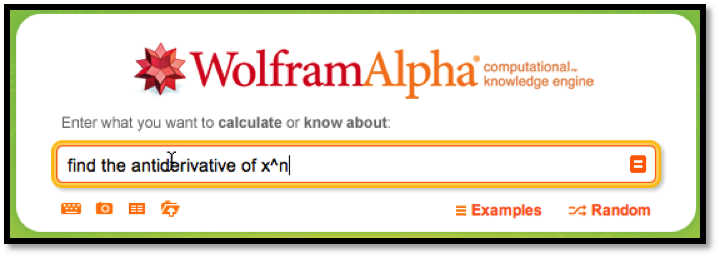
\includegraphics[width=\linewidth]{images/sec7-5-1.png}
\end{sbspanel}%
\end{sidebyside}%
\par
The Alpha provides an answer.%
\begin{sidebyside}{1}{0.15}{0.15}{0}%
\begin{sbspanel}{0.7}%
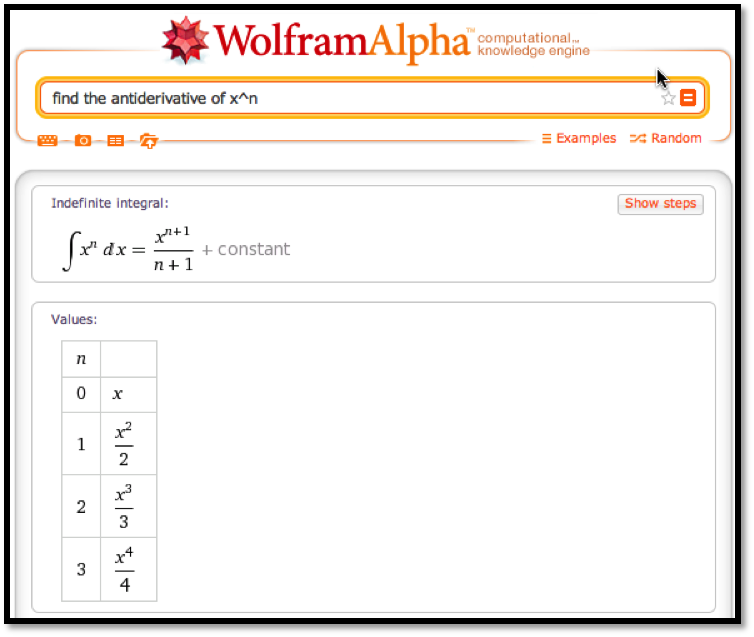
\includegraphics[width=\linewidth]{images/sec7-5-2.png}
\end{sbspanel}%
\end{sidebyside}%
\par
Note that the response tells us the question the Wolfram\textbar{}Alpha is answering.  That helps us check that we have been properly understood.  We may find it useful to give a formula without the extra words.%
\begin{sidebyside}{1}{0.15}{0.15}{0}%
\begin{sbspanel}{0.7}%
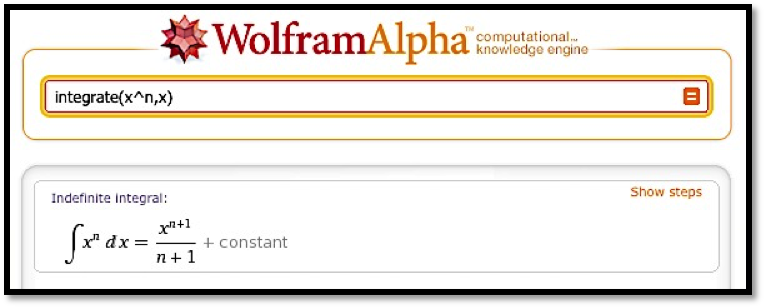
\includegraphics[width=\linewidth]{images/sec7-5-3.png}
\end{sbspanel}%
\end{sidebyside}%
\par
The interface is fairly robust.  It understands the convention that the variable for math problems is typically \(x\), so it will generally guess that x is our variable if we don't specify the variable with respect to which we are integrating.%
\begin{sidebyside}{1}{0.15}{0.15}{0}%
\begin{sbspanel}{0.7}%
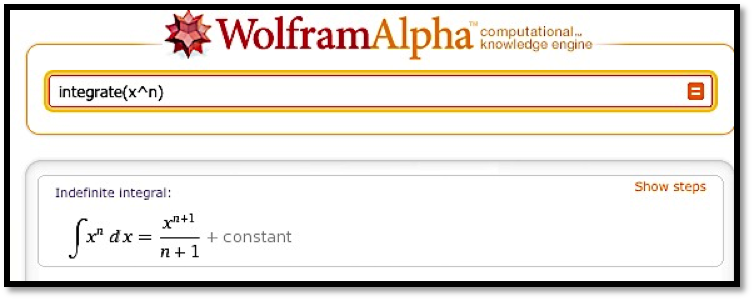
\includegraphics[width=\linewidth]{images/sec7-5-4.png}
\end{sbspanel}%
\end{sidebyside}%
\par
It is worth noting that Wolfram\textbar{}Alpha is connected with Mathematica, so it will understand questions in Mathematica syntax.  On the right side to the screen there is a link for related links.  In particular, there will be a link for the related command in Mathematica.%
\begin{sidebyside}{1}{0.25}{0.25}{0}%
\begin{sbspanel}{0.5}%
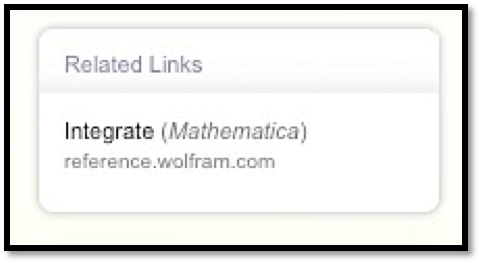
\includegraphics[width=\linewidth]{images/sec7-5-5.png}
\end{sbspanel}%
\end{sidebyside}%
\par
Following that link gives more information on the syntax of the Mathematica command.  We generally don't need to know the syntax, but it is useful if we want to use specific options.%
\begin{sidebyside}{1}{0}{0}{0}%
\begin{sbspanel}{1}%
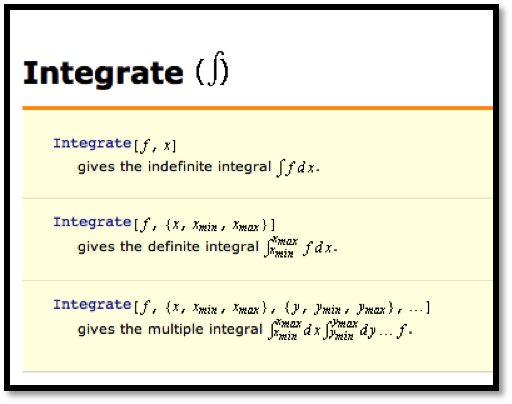
\includegraphics[width=\linewidth]{images/sec7-5-6.png}
\end{sbspanel}%
\end{sidebyside}%
\par
We should note that Wolfram\textbar{}Alpha will easily find antiderivatives that we would find very hard to do or beyond the scope of this class.%
\begin{sidebyside}{1}{0.1}{0.1}{0}%
\begin{sbspanel}{0.8}%
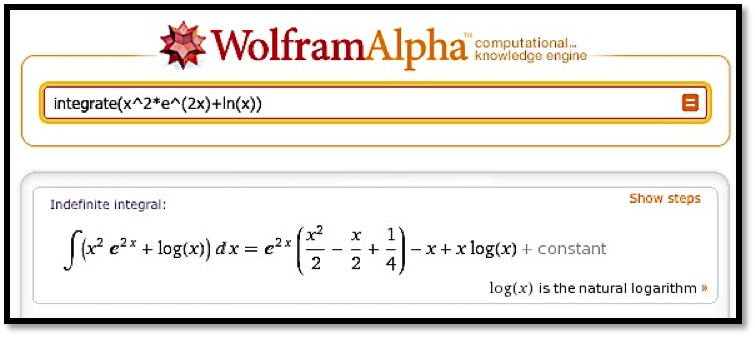
\includegraphics[width=\linewidth]{images/sec7-5-7.png}
\end{sbspanel}%
\end{sidebyside}%
\par
The output also has a link for showing steps on complicated problems.%
\begin{sidebyside}{1}{0.1}{0.1}{0}%
\begin{sbspanel}{0.8}%
\includegraphics[width=\linewidth]{images/sec7-5-8.png}
\end{sbspanel}%
\end{sidebyside}%
\par
The show steps link only works on the paid version of Alpha.  However we can find other tools by searching for integral calculator.  Such a search reveals symbolab, ( https:\slash{}\slash{}www.symbolab.com\slash{}solver\slash{}definite-integral-calculator\textgreater{}, which we also used in chapter 4.%
\begin{sidebyside}{1}{0.05}{0.05}{0}%
\begin{sbspanel}{0.9}%
\includegraphics[width=\linewidth]{images/sec7-5-9.png}
\end{sbspanel}%
\end{sidebyside}%
\par
In chapter 4, we found a derivative calculator.  Similarly we can find an integral calculator (http:\slash{}\slash{}www.integral-calculator.com\slash{}\textgreater{}  that will show steps. For problems of at the level of difficulty we have been doing, Wolfram\textbar{}Alpha also produces plots of the integral.%
\begin{sidebyside}{1}{0.05}{0.05}{0}%
\begin{sbspanel}{0.9}%
\includegraphics[width=\linewidth]{images/sec7-5-10.png}
\end{sbspanel}%
\end{sidebyside}%
\par
\terminology{Definite integrals} - One of the reasons we wanted to find antiderivatives was to be able to use them to evaluate definite integrals.  We can ask Wolfram\textbar{}Alpha for the definite integral directly.  In that case, Wolfram\textbar{}Alpha will give the numeric answer and will also produce the relevant graph.  (Symbolab will also do definite integrals.)%
\begin{sidebyside}{1}{0.05}{0.05}{0}%
\begin{sbspanel}{0.9}%
\includegraphics[width=\linewidth]{images/sec7-5-11.png}
\end{sbspanel}%
\end{sidebyside}%
\par
This is particularly useful when finding the antiderivative is beyond the scope of this course.  Consider for example if we want to find the area under a portion of a curve that has the shape of a normal curve.%
\begin{sidebyside}{1}{0.05}{0.05}{0}%
\begin{sbspanel}{0.9}%
\includegraphics[width=\linewidth]{images/sec7-5-12.png}
\end{sbspanel}%
\end{sidebyside}%
\par
Another example when we can easily set up integrals we cannot solve by hand occurs when we are trying to find the current value of a revenue stream.  A value, \(V\), that we get \(t\) years in the future, has a present value of \(V exp(-r t)\) where \(r\) is an investment return rate.  Thus the current value of a revenue stream, \(V(t)\), from time \(a\) to time \(b\), is \(\int_a^b V(t)*e^{(-r*t)} dt\).  However we only have a rule for finding the antiderivative when \(V(t)\) is either a constant or exponential function.  With a CAS program it is straightforward to compute such integrals for a broad range of value stream functions.%
\begin{sidebyside}{1}{0.1}{0.1}{0}%
\begin{sbspanel}{0.8}%
\includegraphics[width=\linewidth]{images/sec7-5-13.png}
\end{sbspanel}%
\end{sidebyside}%
\par
If you are going to use Wolfram\textbar{}Alpha in doing work, you should realize that the terms of use of the site require you to appropriately cite Wolfram\textbar{}Alpha.  (This is standard academic procedure.)  Your citation should include that date that you got your answer from the site.  The results above were obtained on Feb 29, 2012.%
\par
In business situations, we are rarely asked to simply find an integral.  Instead, finding an integral is generally part of a larger problem.  Thus we often use CAS for part of a problem.%
\par
\terminology{Initial value problems} - We often want to choose a particular antiderivative of a function.  We typically do this when we have the value of the antiderivative for some value.  We simply plug that value into the general antiderivative and solve for \(C\).%
\begin{example}{Finding the antiderivative, then the constant.}{g:example:idm291741075184}%
The rate of change profit with respect to quantity is given by \(P' (q)=-q^2+5q+50\) and the break-even point occurs when \(q=5\).  Find the formula for profit as a function of \(q\).  Find the maximum profit.%
\par
We can do this by putting together things we have already done.  First we use Wolfram\textbar{}Alpha to find an antiderivative.%
\begin{sidebyside}{1}{0.15}{0.15}{0}%
\begin{sbspanel}{0.7}%
\includegraphics[width=\linewidth]{images/sec7-5-14.png}
\end{sbspanel}%
\end{sidebyside}%
\par
Thus we know \(P(q)=\frac{1q^3}{3}+\frac{5q^2}{2}+50q+C\) for some constant \(C\).  We also know \(P(5)=0\).  We now plug the function, without the \(C\), into Excel and evaluate at \(q=5\).%
\begin{sidebyside}{1}{0.15}{0.15}{0}%
\begin{sbspanel}{0.7}%
\includegraphics[width=\linewidth]{images/sec7-5-15.png}
\end{sbspanel}%
\end{sidebyside}%
\par
We make C the negative of our answer and modify our function accordingly.  We now use solver to maximize the function.%
\begin{sidebyside}{1}{0.15}{0.15}{0}%
\begin{sbspanel}{0.7}%
\includegraphics[width=\linewidth]{images/sec7-5-16.png}
\end{sbspanel}%
\end{sidebyside}%
\par
Thus the maximum profit is \textdollar{}145.83, and it occurs when \(q=10\).%
\end{example}
\begin{example}{The previous example in one step.}{g:example:idm291741063424}%
The rate of change profit with respect to quantity is given by \(P' (q)=-q^2+5q+50\) and the break-even point occurs when \(q=5\).  Find the formula for profit as a function of \(q\).  Find the maximum profit.%
\par
We can also do this with Wolfram\textbar{}Alpha setting up the boundary value problem.  We give the alpha bot the derivative we want integrated and the fixed value of the original function.  (Notice that the answer does not include a +C, since we have computed a particular constant.)%
\begin{sidebyside}{1}{0.15}{0.15}{0}%
\begin{sbspanel}{0.7}%
\includegraphics[width=\linewidth]{images/sec7-5-17.png}
\end{sbspanel}%
\end{sidebyside}%
\begin{sidebyside}{1}{0.15}{0.15}{0}%
\begin{sbspanel}{0.7}%
\includegraphics[width=\linewidth]{images/sec7-5-18.png}
\end{sbspanel}%
\end{sidebyside}%
\par
We then ask Alpha to maximize the function.%
\begin{sidebyside}{1}{0.05}{0.05}{0}%
\begin{sbspanel}{0.9}%
\includegraphics[width=\linewidth]{images/sec7-5-19.png}
\end{sbspanel}%
\end{sidebyside}%
\par
This gives the same answer of \textdollar{}145.83.%
\end{example}
This first example could easily have been done by hand.  We can repeat the process with an example that could not be easily been by hand.%
\begin{example}{A more complicated initial value problem.}{g:example:idm291741054080}%
The rate of change of profit with respect to quantity is given by \(P' (q)=q^2  \exp(-q/10)-q/10\) and a break-even point occurs when \(q = 5\).  Find the formula for profit as a function of \(q\).  Find the maximum profit.%
\par
In structure, this example is very similar to the first example.  However, where in the first example, the function would have been easy to do by hand, in this case, the problem is very hard to do by hand.  We use Wolfram\slash{}Alpha to find the antiderivative.%
\begin{sidebyside}{1}{0.15}{0.15}{0}%
\begin{sbspanel}{0.7}%
\includegraphics[width=\linewidth]{images/sec7-5-20.png}
\end{sbspanel}%
\end{sidebyside}%
%
\begin{equation*}
P(q) = exp(-q/10)*(-10*q^2-200*q-2000)-q^2/20+C.
\end{equation*}
We then use Excel to find \(C\), noting that if we use \(P(q)\) without the \(C\), then \(C\) is the value of \(–P(5) = 1972.474\).%
\begin{sidebyside}{1}{0.15}{0.15}{0}%
\begin{sbspanel}{0.7}%
\includegraphics[width=\linewidth]{images/sec7-5-21.png}
\end{sbspanel}%
\end{sidebyside}%
\par
We plug in 5 and note \(P(5) = 0 = C-1972.474\), thus \(C = 1972.474\).  We use solver to maximize and find the maximum profit of \textdollar{}1675.17 occurs at \(q=64.72775\).%
\begin{sidebyside}{1}{0.05}{0.05}{0}%
\begin{sbspanel}{0.9}%
\includegraphics[width=\linewidth]{images/sec7-5-22.png}
\end{sbspanel}%
\end{sidebyside}%
\end{example}
Riemann sums - We can also use Alpha to do Riemann sums.  We need to give a starting and ending point and the number of intervals.%
\begin{example}{Riemann sums with Wolfram\textbar{}Alpha.}{g:example:idm291741040864}%
Find the current value of a revenue stream \(V(t)=2000+5t\) for 10 years with an investment rate of \(r=1.03\), assuming payments are made daily.%
\par
We approximate the current value with the integral%
%
\begin{equation*}
CurrentValue=\int_{start}^{stop} r^{-t} V(t)dt= \int_0^{10} 1.03^{-t} (2000+5t)dt.
\end{equation*}
What we really want is the Riemann sum with one interval per day.  Over 10 years we have 3652 days.%
\begin{sidebyside}{1}{0.15}{0.15}{0}%
\begin{sbspanel}{0.7}%
\includegraphics[width=\linewidth]{images/sec7-5-23.png}
\end{sbspanel}%
\end{sidebyside}%
\begin{sidebyside}{1}{0.15}{0.15}{0}%
\begin{sbspanel}{0.7}%
\includegraphics[width=\linewidth]{images/sec7-5-24.png}
\end{sbspanel}%
\end{sidebyside}%
\par
If we assume payments start at the beginning of the first day we would use the left endpoint method.%
\end{example}
%
%
\typeout{************************************************}
\typeout{Exercises 1.5.1 Exercises: Integration using Computer Algebra Problems}
\typeout{************************************************}
%
\begin{exercises-subsection}{Exercises: Integration using Computer Algebra Problems}{}{Exercises: Integration using Computer Algebra Problems}{}{}{x:exercises:exercises-set-sec-7-5}
For 1-10, find the antiderivative of the given function%
\begin{divisionexercise}{1}{}{}{g:exercise:idm291741032208}%
%
\begin{equation*}
f(x)=x \ln(x)
\end{equation*}
\par\smallskip%
\noindent\textbf{Solution}.\hypertarget{g:solution:idm291741031536}{}\quad{}%
\begin{equation*}
\int x \ln(x)dx=\frac{1}{4} x^{2}(2\ln(x)-1) +c
\end{equation*}
\end{divisionexercise}%
\begin{divisionexercise}{2}{}{}{g:exercise:idm291741030672}%
%
\begin{equation*}
f(t)=e^{.07t} (-t^2+3t+5)
\end{equation*}
\end{divisionexercise}%
\begin{divisionexercise}{3}{}{}{g:exercise:idm291741030016}%
%
\begin{equation*}
f(t)=t^2 e^(-0.06t)
\end{equation*}
\par\smallskip%
\noindent\textbf{Solution}.\hypertarget{g:solution:idm291741029472}{}\quad{}%
\begin{equation*}
\int t^2 e^{-0.06 t} dt= e^{-0.06t} (-9259.26 - 555.556 t - 16.6667 t^2)+c
\end{equation*}
\end{divisionexercise}%
\begin{divisionexercise}{4}{}{}{g:exercise:idm291741028720}%
%
\begin{equation*}
f(x)=\ln(x)
\end{equation*}
\end{divisionexercise}%
\begin{divisionexercise}{5}{}{}{g:exercise:idm291741028048}%
%
\begin{equation*}
f(t)=(t+1) e^{-0.06t}
\end{equation*}
\par\smallskip%
\noindent\textbf{Solution}.\hypertarget{g:solution:idm291741027504}{}\quad{}%
\begin{equation*}
\int (t+1) e^{-0.06t}\ dt =e^(-0.06t) (-294.444 - 16.6667 t)+c
\end{equation*}
\end{divisionexercise}%
\begin{divisionexercise}{6}{}{}{g:exercise:idm291741026768}%
%
\begin{equation*}
f(x)=\frac{1}{(1+2x)(3+x)(5+6x) }
\end{equation*}
\end{divisionexercise}%
\begin{divisionexercise}{7}{}{}{g:exercise:idm291741026064}%
%
\begin{equation*}
f(x)=\frac{1}{\sqrt{1+x^2}}
\end{equation*}
\par\smallskip%
\noindent\textbf{Solution}.\hypertarget{g:solution:idm291741025520}{}\quad{}%
\begin{equation*}
\int \frac{1}{\sqrt{1+x^2}}\ dx= \sinh^{-1}(x)+c
\end{equation*}
\end{divisionexercise}%
\begin{divisionexercise}{8}{}{}{g:exercise:idm291741024784}%
%
\begin{equation*}
f(x)=\frac{1}{(3+2x)^2} 
\end{equation*}
\end{divisionexercise}%
\begin{divisionexercise}{9}{}{}{g:exercise:idm291741024096}%
%
\begin{equation*}
f(x)=\frac{5}{9+x^2 }
\end{equation*}
\par\smallskip%
\noindent\textbf{Solution}.\hypertarget{g:solution:idm291741023552}{}\quad{}%
\begin{equation*}
\int \frac{5}{9+x^2 }\ dx = \left(\frac{5}{3}\right)\tan^{-1}\left(\frac{x}{3}\right)+c
\end{equation*}
\end{divisionexercise}%
\begin{divisionexercise}{10}{}{}{g:exercise:idm291741022784}%
%
\begin{equation*}
f(x)=\frac{1}{(5x+4)^2 (7x+9)}
\end{equation*}
\end{divisionexercise}%
For problems 11-16 evaluate the definite integral.%
\begin{divisionexercise}{11}{}{}{g:exercise:idm291741021632}%
%
\begin{equation*}
\int_0^{10} t^2 e^{-0.06t}  dt 
\end{equation*}
\par\smallskip%
\noindent\textbf{Solution}.\hypertarget{g:solution:idm291741021072}{}\quad{}%
\begin{equation*}
\int_0^{10} t^2 e^{-0.06t}  dt \approx 214.03
\end{equation*}
\end{divisionexercise}%
\begin{divisionexercise}{12}{}{}{g:exercise:idm291741020208}%
%
\begin{equation*}
\int_1^{10}\frac{dt}{t} 
\end{equation*}
\end{divisionexercise}%
\begin{divisionexercise}{13}{}{}{g:exercise:idm291741019376}%
%
\begin{equation*}
\int_1^8(x-1)(x-8)  dx
\end{equation*}
\par\smallskip%
\noindent\textbf{Solution}.\hypertarget{g:solution:idm291741018688}{}\quad{}%
\begin{equation*}
\int_1^8(x-1)(x-8)  dx \approx -57.167
\end{equation*}
\end{divisionexercise}%
\begin{divisionexercise}{14}{}{}{g:exercise:idm291741017824}%
%
\begin{equation*}
\int_0^{10}t^2 e^{.05(10-t)}  dt 
\end{equation*}
\end{divisionexercise}%
\begin{divisionexercise}{15}{}{}{g:exercise:idm291741017120}%
%
\begin{equation*}
\int_0^2 e^{-x^2} dx
\end{equation*}
\par\smallskip%
\noindent\textbf{Solution}.\hypertarget{g:solution:idm291741016576}{}\quad{}%
\begin{equation*}
\int_0^2 e^{-x^2} dx \approx 0.882081
\end{equation*}
\end{divisionexercise}%
\begin{divisionexercise}{16}{}{}{g:exercise:idm291741015712}%
%
\begin{equation*}
\int_9^{16} \frac{1}{\sqrt{2\pi}} e^{-(x-10)^2}  dx 
\end{equation*}
\end{divisionexercise}%
For problems 17-20 do the initial value problem.%
\begin{divisionexercise}{17}{}{}{g:exercise:idm291741014528}%
%
\begin{equation*}
P' (q)=-q^2+3q+5\hbox{ and }P(3)=5.\hbox{ Find } P(q)
\end{equation*}
\par\smallskip%
\noindent\textbf{Solution}.\hypertarget{g:solution:idm291741013952}{}\quad{}%
\begin{equation*}
P(q)=\frac{1}{6} (-2q^3+9q^2+30q-87)
\end{equation*}
\end{divisionexercise}%
\begin{divisionexercise}{18}{}{}{g:exercise:idm291741013088}%
%
\begin{equation*}
F' (t)=t^2 e^{-0.1t} \hbox{ and } F(10)=2.  \hbox{ Find } F(t).
\end{equation*}
\end{divisionexercise}%
\begin{divisionexercise}{19}{}{}{g:exercise:idm291741012352}%
%
\begin{equation*}
P' (q)=\sqrt{q^2+5q+7} \hbox{ and } P(0)=7.  \hbox{ Find } P(q).
\end{equation*}
\par\smallskip%
\noindent\textbf{Solution}.\hypertarget{g:solution:idm291741011760}{}\quad{}%
\begin{equation*}
P(q) = (56 - 50 \sqrt{157} + (4q+10) \sqrt{7 + 5 q + q^2} 
\end{equation*}
%
\begin{equation*}
- 3 \sinh^{-1}\left(\frac{25}{\sqrt{3}}\right)+ 3 \sinh^{-1}\left(\frac{5 + 2 q}{\sqrt{3}}\right))/8
\end{equation*}
\end{divisionexercise}%
\begin{divisionexercise}{20}{}{}{g:exercise:idm291741010512}%
%
\begin{equation*}
P' (q)=-(q^2+2q+3)^2 \hbox{ and } P(10)=-7.  \hbox{ Find } P(q).
\end{equation*}
\end{divisionexercise}%
\begin{divisionexercise}{21}{}{}{g:exercise:idm291741009776}%
I have an investment that produces income at a rate of \(P(t)=5000+100t\).  I assume the present value of an asset decreases continuously at a rate of 2\% per year for the length of time I have to wait for the asset.  What is the present value of the first 7 years of return from my investment?%
\par\smallskip%
\noindent\textbf{Solution}.\hypertarget{g:solution:idm291741008576}{}\quad{}%
\begin{equation*}
\int_0^7(5000+100t) (.98)^t dt\approx 34868.6
\end{equation*}
\end{divisionexercise}%
\begin{divisionexercise}{22}{}{}{g:exercise:idm291741007712}%
My oil well is producing revenue at a rate of \(P(t)=5000(0.09^t)\).  I assume the present value of an asset decreases continuously at a rate of 3\% per year for the length of time I have to wait for the asset.  What is the present value of the first 10 years of return from my investment?%
\end{divisionexercise}%
\begin{divisionexercise}{23}{}{}{g:exercise:idm291741006368}%
The rate of marginal profit is \(MP(q)=100-12\ln(q)\) and a break-even point occurs at \(q=100\). Find the quantity that produces the most profit and the amount of profit generated at that point.%
\par\smallskip%
\noindent\textbf{Solution}.\hypertarget{g:solution:idm291741004832}{}\quad{}We have maximal profit when \(MP(q)=0\), or when \(q=e^8=2981\).%
\par
Using WolframAlpha to solve the initial value problem we get%
%
\begin{equation*}
P(q)=16(7q-700+75ln(100))-12q ln(q)
\end{equation*}
%
\begin{equation*}
P(2981)= 16(7*2981-700+75ln(100))-12*2981 ln(2981)=42021.7
\end{equation*}
\end{divisionexercise}%
\begin{divisionexercise}{24}{}{}{g:exercise:idm291741001776}%
Our marginal cost function is \(MC(q)=10q \ln(q)\) and the startup costs are \textdollar{}23,000.  Produce a cost function.%
\end{divisionexercise}%
\end{exercises-subsection}
\end{sectionptx}
%
%
\typeout{************************************************}
\typeout{Section 1.6 The Normal Distribution: An extended numeric example}
\typeout{************************************************}
%
\begin{sectionptx}{The Normal Distribution: An extended numeric example}{}{The Normal Distribution: An extended numeric example}{}{}{x:section:sec-7-6-NormalDistribution}
\href{./Examples/Section-7-6-Examples.xlsx}{Link to worksheets used in this section}%
\par
We want to look at an extended example where we realistically want to find a definite integral, but need to use numerical methods rather than solving for the antiderivative and using the fundamental theorem of calculus. Most students are familiar with the concept of a course that is graded on a curve.  Formally that means that there is a preset distribution of grades available in the class, with a certain percentage of the students getting an A, a certain percentage getting a B, and so forth.  Most college students are also familiar with the ACT, SAT, or other standardized tests, where the grades typically follow a normal or bell curve.  The result we pull from more advanced mathematics is that many phenomena such as height, weight, and hat size, also follow a bell curve.  In a business setting, we are often concerned whether or not a portion of a market will be big enough to support a specialty store.  We also want to know how much of my production should be allocated to a range of sizes of a product.  This question often boils down to finding the area under a specified portion of the normal curve.%
\par
\terminology{Background from probability}%
\par
We want to pull some definitions and results from the theory of probability.  In particular we want a description of the function we are finding the area under and also of the related area function.%
\begin{assemblage}{}{g:assemblage:idm291740996832}%
\terminology{Definition}: A \terminology{Probability Density Function} is a function that spreads the area 1 over the entire real line, with the obvious understanding that no value can have a negative probability.%
\par
In calculus terms, a \terminology{Probability Density Function} is a function  \(f(x)\) defined for \(-\infty\lt x \lt \infty \)  such that \(f(x)\ge 0\)  and  \(\int_{-\infty}^{\infty}f(x)dx=1\).%
\end{assemblage}
A probability density function is also called a continuous distribution function.  The probability density function that is of most interest to us is the normal distribution.  The normal density function is given by%
%
\begin{equation*}
f(x)=\frac{1}{\sigma\sqrt{2\pi}}\exp\left(\frac{-(x-\mu)^2}{2\sigma^2}\right)
\end{equation*}
where sigma, \(\sigma\), and mu, \(\mu\), are respectively the standard deviation and mean of the distribution.  For this course the mean is the center of the distribution and the standard deviation is a measure of how tightly packed the distribution is.  If we set the mean to 0 and the standard deviation to 1 we have the standardized normal distribution, or the familiar bell curve.%
\par
Thus, when I note that the adult men in the United States have a height distribution that is normal with a mean of 70 inches and a standard deviation of 3 inches, the distribution is%
%
\begin{equation*}
f(x)=\frac{1}{3\sqrt{2\pi}}\exp\left(\frac{-(x-70)^2}{2*3^2}\right)
\end{equation*}
\begin{sidebyside}{1}{0.25}{0.25}{0}%
\begin{sbspanel}{0.5}%
\includegraphics[width=\linewidth]{images/sec7-6-1.png}
\end{sbspanel}%
\end{sidebyside}%
\par
Thus finding the percentage of men less than 5 feet tall, reduces to evaluating the appropriate integral.  Since finding the percentage of the population that fits in our market reduces to finding the area under a specified portion of this curve, we are also interested in the anti-derivative of the distribution.%
\begin{assemblage}{}{g:assemblage:idm291740986656}%
\terminology{Definition}: Given a probability density function, \(f(x)\) , the related \terminology{Cumulative Distribution Function},  \(CDFf(x)\), is a function that measures how much area is over the interval  \((-\infty,x]\).%
\par
In calculus terms,  \(CDFf(x)\), the \terminology{Cumulative Distribution Function} of  \(f(x)\), is  \(\int_{-\infty}^x f(t)dt\).%
\end{assemblage}
You will notice the techniques we have for anti-differentiation will not work with the normal distribution.  In fact, the normal distribution has no closed form anti-derivative using the functions we are familiar with.  Thus we need to use numeric methods.%
\begin{example}{Tall men in an area.}{g:example:idm291740981088}%
In the United States, the height of men follows a normal distribution with a mean of 70 inches (5' 10") and a standard deviation of 3 inches.  I want to set up a specialty shop for men who are at least 6’ tall, but no more than 7' tall.  In an area with 100,000 adult men, how big is my potential market?%
\par
\terminology{Solution set up}.  My distribution function is \(\frac{1}{3\sqrt{2\pi}}\exp\left(\frac{-(x-70)^2}{2*3^3}\right)\). Since I have a population of 100,000 and am interested in the men who are between 72 and 84 inches tall, my potential market is%
%
\begin{equation*}
100000\int_{72}^{84} \frac{1}{3\sqrt{2\pi}} \exp\left(\frac{-(x-70)^2}{2*3^2} \right)dx.
\end{equation*}
As an alternative, I can convert the problem so it is expressed in terms of standard deviations.  Then I use the standardized normal distribution and my limits of integration are%
%
\begin{equation*}
low\ bound\ in\ SD = (low\ bound-mean)/(SD) = (72-70)/3 = 2/3
\end{equation*}
%
\begin{equation*}
upper\ bound\ in\ SD = (upper\ bound-mean)/(SD) = (84-70)/3 = 14/3.
\end{equation*}
Then my potential market is%
%
\begin{equation*}
100000\int_{2/3}^{14/3} \frac{1}{\sqrt{2\pi}} \exp(-x^2/2)dx.
\end{equation*}
\terminology{Solution 1, using Excel and Riemann Sums}:  I want to set up a spreadsheet to find the area under the curve.  Since I think I may do this for several problems, I want to set up the worksheet as a template that I can simply fill in.  It will make my life easier if I recast the problem in terms of standard deviations.   My potential market is \(100000\int_{2/3}^{14/3} \frac{1}{\sqrt{2\pi}} \exp(-x^2/2)dx\).   I am ready to set up a Riemann sum worksheet as we did in section 7.1%
\begin{sidebyside}{1}{0.1}{0.1}{0}%
\begin{sbspanel}{0.8}%
\includegraphics[width=\linewidth]{images/sec7-6-2.png}
\end{sbspanel}%
\end{sidebyside}%
\par
In cells F3 through F5 we convert the lower bound, upper bound, and del x to standard deviations.  We recall that we get better accuracy by evaluating the rectangles with a midpoint.  The midpoint of the nth rectangle is (n-0.5)\textasteriskcentered{}del x above the lower bound.  As we did in previous sections, we use the offset command to bring our answer into the top region.  When we look at the numbers we see that the potential market is 25,249.%
\begin{sidebyside}{1}{0.25}{0.25}{0}%
\begin{sbspanel}{0.5}%
\includegraphics[width=\linewidth]{images/sec7-6-3.png}
\end{sbspanel}%
\end{sidebyside}%
\par
\terminology{Solution 1a, using Excel Statistics Commands}:  By this point in the course you should expect that if we claim a computation is important and done by business many times, that there is an Excel command to do the computation.%
\par
The function we are interested in is%
%
\begin{equation*}
\hbox{NORM.DIST(x, mean, standard deviation, cumulative).}
\end{equation*}
Where \(x\), mean, and standard deviation have the obvious meanings.  The cumulative parameter is either true or false.  If it is true we get the cumulative distribution function.  If it is false we get the probability density function.  If we are working with the standardized normal distribution, where the mean is 0 and the standard deviation is 1, the command is%
%
\begin{equation*}
\hbox{NORM.S.DIST(x, cumulative).}
\end{equation*}
(If you are using older versions of Excel, the syntax of the command is a little different.  Check the appropriate help page if you are using an older version of Excel.)  With these commands, our spreadsheet is noticeably simpler.%
\begin{sidebyside}{1}{0.15}{0.15}{0}%
\begin{sbspanel}{0.7}%
\includegraphics[width=\linewidth]{images/sec7-6-4.png}
\end{sbspanel}%
\end{sidebyside}%
\par
When we look at the values, we get a target population of 25,249.  This agrees with our estimate to 5 significant figures.%
\begin{sidebyside}{1}{0.25}{0.25}{0}%
\begin{sbspanel}{0.5}%
\includegraphics[width=\linewidth]{images/sec7-6-5.png}
\end{sbspanel}%
\end{sidebyside}%
\par
\terminology{Solution 1b, using Wolfram alpha}:  Once I have reduced the problem to evaluating a definite integral, I can find a numeric solution with a CAS package like Wolfram\textbar{}Alpha.%
%
\begin{equation*}
100000\int_{72}^{84} \frac{1}{3\sqrt{2\pi}} \exp\left(\frac{-(x-70)^2}{2*3^2 }\right)dx
\end{equation*}
becomes%
100000\textasteriskcentered{}integrate(exp(-(x-70)\textasciicircum{}2\slash{}(2\textasteriskcentered{}3\textasciicircum{}2))\slash{}(3\textasteriskcentered{}sqrt(2\textasteriskcentered{}pi))) from 72 to 84.%
We get our familiar answer of 25,249.%
\begin{sidebyside}{1}{0.2}{0.2}{0}%
\begin{sbspanel}{0.6}%
\includegraphics[width=\linewidth]{images/sec7-6-6.png}
\end{sbspanel}%
\end{sidebyside}%
\par
When we compute a target population, we sometimes want to include the tail of the distribution.  We might, for example be concerned with all women who are 5 feet tall or less.  This sets up an integral over an infinite interval, which we can’t do as a Riemann sum.  The first workaround notes that the tails are very small.  If all humans who have ever lived are normally distributed, less than 1 is more than 7 standard deviations from the mean.  Taking the integral down to -7 will practically be the same as integrating down to \(-\infty\).  The second workaround uses the symmetry of the normal distribution.%
%
\begin{equation*}
\int_{-\infty}^a SND(x)dx=\int_{-\infty}^0 SND(x)dx+\int_0^a SND(x)dx=.5+\int_0^a SND(x)dx.
\end{equation*}
\end{example}
\begin{example}{Finding tall women.}{g:example:idm291740955136}%
In the United States, the height of women follows a normal distribution with a mean of 64 inches (5' 4") and a standard deviation of 2.75 inches.  I want to set up a specialty shop for women who are no more than 5' tall.  In an area with 500,000 adult women, how big is my potential market?%
\par
\terminology{Solution}: Set up.  Using the reasoning as above, I want to estimate my market if it is 50\% of the population plus the percentage between 0 and (-4\slash{}2.75) standard deviations below the mean.%
\par
\terminology{Solution}: Using Excel and Riemann Sums:  One advantage of having set up the first exercise well, it the Riemann sum problem is now a matter of changing the parameters and subtracting from 0.5 before multiplying by the market size.%
\begin{sidebyside}{1}{0.25}{0.25}{0}%
\begin{sbspanel}{0.5}%
\includegraphics[width=\linewidth]{images/sec7-6-7.png}
\end{sbspanel}%
\end{sidebyside}%
\par
We notice that since we are finding the area under the standardized normal distribution from 0 to a negative number, we get a negative area.  Our potential market is composed of 3,645 women.%
\par
\terminology{Solution a}: Using Excel Statistics Commands:  When using the statistics commands, the area function is zero at \(-\infty\).  Thus we simply have to evaluate%
 NORM.S.DIST(right hand limit, cumulative). \begin{sidebyside}{1}{0.2}{0.2}{0}%
\begin{sbspanel}{0.6}%
\includegraphics[width=\linewidth]{images/sec7-6-8.png}
\end{sbspanel}%
\end{sidebyside}%
\par
Once again, we get a potential market of 3,645 women.%
\end{example}
While the normal distribution spreads a population over the real numbers, most objects come in discrete sizes.  Depending on the kind of shoes, the sizes are either whole or half numbers.  You can’t buy a shoe of size 8.764.  The normal procedure is to divide the population at the middle between the sizes.%
\begin{example}{Women's shoes.}{g:example:idm291740945712}%
In the United States, the shoe sizes of women follows a normal distribution with a mean of 8 and a standard deviation of 1.5.  I want to order 1000 pairs of shoes.  If the shoes are only available in full sizes, how many pairs should I order of size 7?%
\par
\terminology{Solution}:  I want the portion of the population between size 6.5 and 7.5.   I fit it into my worksheet for Riemann sums.%
\begin{sidebyside}{1}{0.25}{0.25}{0}%
\begin{sbspanel}{0.5}%
\includegraphics[width=\linewidth]{images/sec7-6-7.png}
\end{sbspanel}%
\end{sidebyside}%
\par
Of the 1000 pairs of shoes, 211 should be size 7.%
\end{example}
We have looked at three methods for finding a portion of a normally distributed population, which we describe as Excel with Riemann sums, Excel with statistics commands, and CAS.  It is worthwhile to consider the advantages and disadvantages of the methods.  The Riemann sums method takes the most work to set up.  It is also conceptually the most straightforward and the most flexible.  It is the easiest to adapt if we are doing some nonstandard distribution of a population.  It also shows intermediate values if we have a less sharp question and are trying to see what is going on and are still deciding on the business question we want to ask.  The Excel with statistics command approach requires us to learn special commands.  It is also less work.  It would probably be the favored method if we were doing a lot of these computations.  It should be noted that Excel has corresponding commands for the other standard probability distributions. The CAS method does not require special commands, but it takes us out of our Excel environment.  It does not let us leave a worksheet that is well documented and that can be easily modified by someone else asking similar questions.%
%
%
\typeout{************************************************}
\typeout{Exercises 1.6.1 Exercises: Normal Distribution Problems}
\typeout{************************************************}
%
\begin{exercises-subsection}{Exercises: Normal Distribution Problems}{}{Exercises: Normal Distribution Problems}{}{}{x:exercises:exercises-set-sec-7-6}
\begin{divisionexercise}{1}{}{}{g:exercise:idm291740940016}%
Assume that women’s shoe sizes are normally distributed with a mean of 8 and a standard deviation of 1.5.  A particular style of shoes in available in full and half sizes.  I plan to make 10,000 pairs of this style.%
%
\begin{enumerate}[label=(\alph*)]
\textgreater{} \item{}Express, as an integral, the number of pairs I should make of size 9.%
\item{}How many pairs of size 9 shoes should I make?%
\item{}How do your answers change if the shoes are only to be made in full sizes?%
\end{enumerate}
\par\smallskip%
\noindent\textbf{Solution}.\hypertarget{g:solution:idm291740936688}{}\quad{}%
\begin{enumerate}[label=(\alph*)]
\textgreater{} \item{}%
\begin{equation*}
\hbox{pairs size 9}=10000\int_{8.75}^{9.25}
\frac{1}{1.5\sqrt{2\pi}}e^{\left({\frac{-(x-9)^2}{2*1.5^2}}\right)}\ dx
\end{equation*}
%
\item{}%
\begin{equation*}
10000\int_{8.75}^{9.25} \frac{1}{1.5\sqrt{2\pi}} e^{\left({\frac{-(x-9)^2}{2*1.5^2}}\right)}\ dx=1062.
\end{equation*}
%
\item{}If we only have full sizes the limits of integration go from 8.5 to 9.5.  I then need 2108 pairs of size 9.%
\end{enumerate}
\end{divisionexercise}%
\begin{divisionexercise}{2}{}{}{g:exercise:idm291740933680}%
Men's shoes in Europe are made if full sizes with a different measuring system than we use in the United States.  They are normally distributed with a mean of 43 and a standard deviation of 2\slash{}3.  I plan to buy 1,000 pairs of shoes for my store.%
%
\begin{enumerate}[label=(\alph*)]
\item{}Express, as an integral, the number of pairs I should order of size 45.%
\item{}Express, as an Excel command, the number of pairs I should order of size 45.%
\item{}How many pairs should I order of size 44?  (Give a number, not an equation.)%
\end{enumerate}
\end{divisionexercise}%
\begin{divisionexercise}{3}{}{}{g:exercise:idm291740930144}%
Assume that women’s dress sizes are normally distributed with a mean of 14 and a standard deviation of 3.  For a particular style, 5000 dresses will be made, and they are available in even integer sizes.  (2, 4, …).%
%
\begin{enumerate}[label=(\alph*)]
\item{}Express, as an integral, the number of dresses I should make of size 10.%
\item{}How many size 6 dresses should I make?%
\item{}How many size 10 dresses should I make?%
\end{enumerate}
\par\smallskip%
\noindent\textbf{Solution}.\hypertarget{g:solution:idm291740926848}{}\quad{}%
\begin{enumerate}[label=(\alph*)]
\item{}%
\begin{equation*}
\hbox{size 10 dresses}=5000\int_{9}^{11}
\frac{1}{3\sqrt{2\pi}}e^{\left({\frac{-(x-14)^2}{2*3^2}}\right)}\ dx
\end{equation*}
%
\item{}%
\begin{equation*}
5000\int_{5}^{7}\frac{1}{3\sqrt{2\pi}} e^{\left({\frac{-(x-14)^2}{2*3^2}}\right)}\ dx = 43
\end{equation*}
%
\item{}%
\begin{equation*}
5000\int_{9}^{11}\frac{1}{3\sqrt{2\pi}} e^{\left({\frac{-(x-14)^2}{2*3^2}}\right)}\ dx = 555
\end{equation*}
%
\end{enumerate}
\end{divisionexercise}%
\begin{divisionexercise}{4}{}{}{g:exercise:idm291740923888}%
Assume that men’s suit coat sizes are normally distributed with a mean of 44 and a standard deviation of 4.  For a particular style, 2000 suit coats will be made, and they are available in even integer sizes.  (2, 4, …).%
%
\begin{enumerate}[label=(\alph*)]
\item{}Express, as an integral, the number of suit coats I should make of size 44.%
\item{}How many size 44 suit coats should I make?%
\end{enumerate}
\end{divisionexercise}%
\begin{divisionexercise}{5}{}{}{g:exercise:idm291740921008}%
A study of the size of male soldiers found the headband lengths were normally distributed with a mean of 22.1 inches and a standard deviation of 0.85 inches.  Standard sized caps will fit headbands lengths of 20-25 inches.%
%
\begin{enumerate}[label=(\alph*)]
\item{}Express, as an integral, the percentage of soldiers for who will fit the standard sized caps.%
\item{}Cap sizes come in quarter sizes with a full size corresponding to a change in headband size of 3 inches, with a size 8 corresponding to 25 inches.  Out of 1,000 soldiers, how many need a size 8 cap?%
\end{enumerate}
\par\smallskip%
\noindent\textbf{Solution}.\hypertarget{g:solution:idm291740918096}{}\quad{}%
\begin{enumerate}[label=(\alph*)]
\item{}%
\begin{equation*}
\hbox{pecentage fit}=100\int_{20}^{25}\frac{1}{0.85\sqrt{2\pi}} e^{\left({\frac{-(x-22.1)^2}{2*0.85^2}}\right)}\ dx =99.29
\end{equation*}
%
\item{}%
\begin{equation*}
\hbox{size 8 caps}=1000\int_{24.625}^{25.375}\frac{1}{0.85\sqrt{2\pi}} e^{\left({\frac{-(x-22.1)^2}{2*0.85^2}}\right)}\ dx =1.42
\end{equation*}
%
\end{enumerate}
\end{divisionexercise}%
\begin{divisionexercise}{6}{}{}{g:exercise:idm291740915696}%
A study of the size of male soldiers found the hip breadths were normally distributed with a mean of 13.45 inches and a standard deviation of 0.64 inches.  Seats on one airline measure 17 inches between the armrests.  Express, as an integral, the percentage of soldiers who hips are too wide for the seats.%
\end{divisionexercise}%
\begin{divisionexercise}{7}{}{}{g:exercise:idm291740914720}%
Assume that women’s shoe sizes are normally distributed with a mean of 8 and a standard deviation of 1.5.  A particular style of shoes is available in full and half sizes.  I plan to make 1,000 pairs of this style.  Using the Excel statistics commands, make a chart telling me many pairs I should make of each size.%
\par\smallskip%
\noindent\textbf{Solution}.\hypertarget{g:solution:idm291740913872}{}\quad{}Since the shoes come in half sizes, we want the area under the normal distribution function from 0.25 before the given size to 0.25 after the given size.%
\par
The desired syntax is%
\par
Population size \textasteriskcentered{} (NORM.DIST(Size+0.25, Mean, Standard Deviation, TRUE) - NORM.DIST(Size+0.25, Mean, Standard Deviation, TRUE) )%
\begin{sidebyside}{1}{0.1}{0.1}{0}%
\begin{sbspanel}{0.8}%
\includegraphics[width=\linewidth]{images/sec7-6-sol7a.png}
\end{sbspanel}%
\end{sidebyside}%
\begin{sidebyside}{1}{0.3}{0.3}{0}%
\begin{sbspanel}{0.4}%
\includegraphics[width=\linewidth]{images/sec7-6-sol7b.png}
\end{sbspanel}%
\end{sidebyside}%
\end{divisionexercise}%
\begin{divisionexercise}{8}{}{}{g:exercise:idm291740908752}%
Assume that men’s suit coat sizes are normally distributed with a mean of 44 and a standard deviation of 4.  For a particular style, 2,000 suit coats will be made, and they are available in even integer sizes.  (2, 4, …). Using the Excel statistics commands, make a chart telling me many suits I should make of each size.%
\end{divisionexercise}%
\begin{divisionexercise}{9}{}{}{g:exercise:idm291740907760}%
Assume that results on an intelligence test are normally distributed with a mean of 100 and a standard deviation of 15.  Using the Excel statistics commands, make a chart distributing 1,000,000 people between intervals of size 10 (90-100, 100-110, etc.).  What is the highest IQ score I should expect to find in my population of 1 million?%
\par\smallskip%
\noindent\textbf{Solution}.\hypertarget{g:solution:idm291740906896}{}\quad{}We set the ranges with a high value and a low value.%
\par
The desired syntax is%
\par
Population size \textasteriskcentered{} (NORM.DIST(High value, Mean, Standard Deviation, TRUE) - NORM.DIST(Low value, Mean, Standard Deviation, TRUE) )%
\begin{sidebyside}{1}{0.1}{0.1}{0}%
\begin{sbspanel}{0.8}%
\includegraphics[width=\linewidth]{images/sec7-6-sol9a.png}
\end{sbspanel}%
\end{sidebyside}%
\begin{sidebyside}{1}{0.3}{0.3}{0}%
\begin{sbspanel}{0.4}%
\includegraphics[width=\linewidth]{images/sec7-6-sol9b.png}
\end{sbspanel}%
\end{sidebyside}%
\par
With a million people, the high IQ should be between 170 and 180.%
\end{divisionexercise}%
\begin{divisionexercise}{10}{}{}{g:exercise:idm291740901360}%
I have been informed that the distance from the back of a chair to the front of the knee of a man sitting is normally distributed with a mean of 24 inches and a standard deviation of 1.3 inches.  I want to design airline chairs to fit 99\% of the male passengers with 1 inch between the knee and the back of the next chair.  How much distance do I need between the front of one chair seat and the back of the next?%
\end{divisionexercise}%
\begin{divisionexercise}{11}{}{}{g:exercise:idm291740900272}%
I have been informed that the breadth at the shoulders of an adult male is normally distributed with a mean of 17.9 inches and a standard deviation of 1 inch.  The standard coach seat on a plane is 17.2 inches wide.  What percentage of adult males fit in such a seat without overflow?%
\par\smallskip%
\noindent\textbf{Solution}.\hypertarget{g:solution:idm291740899472}{}\quad{}%
\begin{equation*}
\hbox{pecentage fit}=100\int_{0}^{17.2}\frac{1}{1\sqrt{2\pi}} e^{\left({\frac{-(x-17.9)^2}{2*1^2}}\right)}\ dx =24.196
\end{equation*}
\end{divisionexercise}%
\begin{divisionexercise}{12}{}{}{g:exercise:idm291740898528}%
The techniques used in this section can easily be adapted to other distributions.  For example, the mean time to failure of a brand of hard drives, measured in units of 10,000 hours, has been found to follow a Weibull distribution with shape variable 3 and scale variable 5.  The probability density function of failure is%
%
\begin{equation*}
FailureDensity(x)=(3/5) (x/5)^2 \exp(-(x/5)^3 ).
\end{equation*}
%
\begin{enumerate}[label=(\alph*)]
\item{}Our warranty is for 10,000 hours of use.  (This is approximately 1 year.)  What percentage of drives get replaced under warrantee?%
\item{}We offer an extended warrantee that replaces the hard drive if it fails in under 30,000 hours of use.  What percentage of users who buy the extended warranty will have their hard drive fail in the period of time between the expiration of the original warrantee and the end of the extended warranty?%
\item{}Some credit cards double the manufacturer’s warranty.  What percentage of the people who use this plan will have their hard drive replaced by the credit card company?%
\item{}What percentage of customers see their hard drives last for 100,000 hours of use?%
\end{enumerate}
\end{divisionexercise}%
\begin{divisionexercise}{13}{}{}{g:exercise:idm291740893584}%
– Project – Pick a product and find evidence on the kind of function that describes its failure rate.  Based on that data, determine how long we expect it to take until 10\% , 50\% , and 90\%  of the products fail.%
\end{divisionexercise}%
\end{exercises-subsection}
\end{sectionptx}
%
%
\typeout{************************************************}
\typeout{Section 1.7 Applications of the integral: Investment and depreciation}
\typeout{************************************************}
%
\begin{sectionptx}{Applications of the integral: Investment and depreciation}{}{Applications of the integral: Investment and depreciation}{}{}{x:section:sec-7-7-InvestmentDepreciation}
\href{./Examples/Section-7-7-Examples.xlsx}{Link to worksheets used in this section}%
\par
Having looked at several ways to evaluate definite integrals, we return to practical problems that we can solve be evaluating an integral.  We will break our applications in this section into two groups.  Problems in the first group reduce to accumulation over time, and are analogous to finding the area under a curve, or finding a definite integral.  Problems in the second group ask you to find a specific anti-derivative of a function.  They are called boundary value problems.%
\par
\terminology{Basic Accumulation}– The most straightforward problem for integration is one where I have a function for some value, like an income stream, or materials produced, or a cost, and I am interested if calculating how much accumulates in a specified interval.  We work through a series of examples where the accumulation function gets progressively more complicated.%
\begin{example}{Accumulating a constant function over time.}{g:example:idm291740888416}%
Mary runs a small shop that is temporarily disconnected from the power network.  A generator that provides power uses 2 gallons of fuel per hour.  How much fuel does she need to keep the shop running from 8 in the morning until 6 in the afternoon.%
\par
\terminology{Solution}: We started with a problem that is easy to do without calculus to give us confidence in our method.  We solve it with algebra first.  Mary wants to run the generator for 10 hours and it consumes 2 gallons of fuel per hour.  She needs (10 hours)(2 gallons\slash{}hour) = 20 gallons of fuel.%
\par
To set the problem up for calculus, we use a 24-hour clock to put time on a number line.  We are accumulating \(FuelConsumption(t)=2\) from \(t=8\) to \(t=18\).  We need%
%
\begin{equation*}
\int_8^{18} 2 dt=|2t|_8^{18}=(2*18)-(2*8)=20
\end{equation*}
gallons of fuel.%
\begin{sidebyside}{1}{0.15}{0.15}{0}%
\begin{sbspanel}{0.7}%
\includegraphics[width=\linewidth]{images/sec7-7-1.png}
\end{sbspanel}%
\end{sidebyside}%
\end{example}
\begin{example}{Accumulating marginal cost.}{g:example:idm291740881824}%
%
\begin{equation*}
Marginal Cost(quantity)=50+quantity/1000
\end{equation*}
Find the increase in cost as production goes from 50,000 to 80,000.%
\par
\terminology{Solution}: Since the change in cost looks like a Riemann sum with 30,000 intervals, we will approximate the change in cost with the integral of the marginal cost.  With this function we can easily find an antiderivative and evaluate. The change in cost is%
%
\begin{equation*}
\int_{50000}^{80000} 50+\frac{q}{1000} dq=
\left.\left( 
50q+\frac{q^2}{2000}
\right)\right|_{50000}^{80000}
\end{equation*}
%
\begin{equation*}
=(7,200,000)-(3,750,000)=3,450,000.
\end{equation*}
The change in cost of production is \textdollar{}3,450,000.%
\begin{sidebyside}{1}{0.25}{0.25}{0}%
\begin{sbspanel}{0.5}%
\includegraphics[width=\linewidth]{images/sec7-7-2.png}
\end{sbspanel}%
\end{sidebyside}%
\end{example}
\begin{example}{Oil production.}{g:example:idm291740876096}%
An oil well in Texas initially produces oil at a rate of 2 million barrels of oil per year.  The production rate will typically fall 15\% per year.  How much oil is produced over a 5-year period?%
\par
\terminology{Solution}: We want to integrate our production rate of \(2(0.85)^t\) as \(t\) goes from 0 to 5.  We can use our antidifferentiation formulas for this problem.%
%
\begin{equation*}
\int_0^5 2(0.85)^t   dt= \left.\left(\frac{2(0.85)^t}{\ln (0.85)}\right)\right|_0^5=\frac{2}{\ln (0.85)}  (0.85^5-1)=6.846.
\end{equation*}
Over 5 years, the well will produce 6.846 million barrels of oil.%
\begin{sidebyside}{1}{0.3}{0.3}{0}%
\begin{sbspanel}{0.4}%
\includegraphics[width=\linewidth]{images/sec7-7-3.png}
\end{sbspanel}%
\end{sidebyside}%
\end{example}
\begin{example}{Discounted revenue stream.}{g:example:idm291740870416}%
Your company is interested in acquiring a revenue stream that is currently producing are a rate of 50+5 t  thousand dollars per year, where t is measured in years.  To obtain current value, you are discounting at a rate of 6\%\slash{}year compounded continuously.  What is the current value of the first 10 years of income from the stream?%
\par
\terminology{Solution}: To find the total income we would want to integrate \((50+5t)\) as \(t\) goes from 0 to 10.  To find the current value we must discount the income based in when we receive it.  Thus we want to integrate \((50+5t) e^{-0.06t}\) as \(t\) goes from 0 to 10.  We set up the integral \(\int_0^{10} (50+5t) e^{-0.06t}  dt\).  Since we do not know how to find the anti-derivative for this function, we find the area either with Excel and Riemann sums, or with Wolfram Alpha.%
\begin{sidebyside}{1}{0.1}{0.1}{0}%
\begin{sbspanel}{0.8}%
\includegraphics[width=\linewidth]{images/sec7-7-4.png}
\end{sbspanel}%
\end{sidebyside}%
\par
With either method, we find that the present value of the revenue stream to be \textdollar{}545,298.%
\begin{sidebyside}{1}{0.25}{0.25}{0}%
\begin{sbspanel}{0.5}%
\includegraphics[width=\linewidth]{images/sec7-7-5.png}
\end{sbspanel}%
\end{sidebyside}%
\end{example}
\terminology{Boundary value problems}: The accumulation problems asked you to find the area under a curve between two specific points.  For those problems, we are not interested in a formulation of a general area function.  A second set of applications starts with a derivative and is interested in finding the particular anti-derivative that meets certain initial conditions.  (We use the conditions to find the correct value of "+C" in the general anti-derivative.)  These problems are often solved once to find the general anti-derivative for a particular kind of problem, and the general solution is then used as a formula to find the constant C.%
\begin{example}{Proportional growth and continuous reinvestment.}{g:example:idm291740860656}%
I put \textdollar{}20,000 in a retirement account that earns 4\% interest compounded continuously.  I reinvest all my earnings from the account back into the retirement account.   I would like a simple formula for the principal at sometime in the future.%
\par
\terminology{Solution}: We already have the formula for continuous growth, but it is worthwhile to derive it again.  We are told%
%
\begin{equation*}
Principal' (time)=.05*Principal(time)
\end{equation*}
or%
%
\begin{equation*}
\frac{Principal' (time)}{Principal(time)}=.05
\end{equation*}
Integrating both sides with respect to time, we get%
%
\begin{equation*}
\ln (Principal(time))=.05*time+C
\end{equation*}
Exponentiating both sides gives%
%
\begin{equation*}
Principal(time)=\exp(0.05*time)*\exp(C)=e^C e^{.05*time}.
\end{equation*}
Since we know that the Principal is \textdollar{}20,000 at time 0, we see that \(e^C=20000\) and our equation simplifies to%
%
\begin{equation*}
Principal(time)=20000e^{.05*time}.
\end{equation*}
This is the formula we took on faith in the last chapter.%
\end{example}
\terminology{Depreciation} When computing costs of a business, we need to evaluate the depreciation cost of capital equipment.  There are a number of reasonable ways of computing depreciation.%
%
\begin{itemize}[label=\textbullet]
\item{}\terminology{Straight-line depreciation}, which assumes that a piece of equipment loses the same amount of value each year until it is worthless.%
\begin{assemblage}{}{g:assemblage:idm291740851184}%
%
\begin{equation*}
Annual\ Depreciation\ Expense=  \frac{Cost\ of\ fixed\ Asset-Residual\ Value}{Useful\ life\ of\ Asset\ (in\ years)}
\end{equation*}
%
\end{assemblage}
\item{}\terminology{The sum of digits method of depreciation}.  It assumes the rate of depreciation is proportional to the expected remaining useful life of the piece of equipment. For example with a sum of years method and defining V(t) as the value, EL is the expected lifetime, k is a constant, and t is time, we would have:%
\begin{assemblage}{}{g:assemblage:idm291740849152}%
%
\begin{equation*}
V' (t)= -k (EL-t)
\end{equation*}
%
\end{assemblage}
\item{}\terminology{The declining balance depreciation}.  This method assumes the rate of depreciation is proportional to the current value, with the initial rate of depreciation twice the straight-line rate, with depreciation stopping when the value is the scrap value. We let N be the estimated life of the asset and we let the rate of depreciation be:%
\begin{assemblage}{}{g:assemblage:idm291740847184}%
%
\begin{equation*}
Depreciation\ rate=1- \sqrt[N]{
\frac{residual\ value}{cost\ of\ fixed\ asset}}
\end{equation*}
%
\end{assemblage}
\end{itemize}
\begin{example}{Straight Line Depreciation.}{g:example:idm291740846288}%
You buy a car for \textdollar{}18,000 and you want to depreciate it to \textdollar{}0 over 5 years. Find a formula for the value of the car. We assume the value decreases a constant rate, so we use straight-line depreciation.  Give a simple formula to find the book value of the equipment after 3.5 years.%
\par
\terminology{Solution}: The easiest way to do this problem is not to use calculus, but to realize we want the equation of a line and we have two points.%
%
\begin{equation*}
Value(0)=18000 \hbox{ and } Value(5)=0.
\end{equation*}
Taking slope as rise over run, the slope is -3,600 and the intercept is 18,000.  Thus our equation is%
%
\begin{equation*}
Value(time)=18000-3600*time.
\end{equation*}
%
\begin{equation*}
Value(3.5)=5,400.
\end{equation*}
Using calculus on the same problem we have%
%
\begin{equation*}
Value' (time)=-k\hbox{ for some constant }k, 
\end{equation*}
%
\begin{equation*}
Value(0)=18000\hbox{ and } Value(5)=0.
\end{equation*}
. Integrating the first equation gives%
%
\begin{equation*}
Value(time)=-k*time+C.
\end{equation*}
Thus, straight-line depreciation gives a value function, which is a straight line.  We now plug in known values to find the constants.  We plug in for \(time = 0\) to see \(C = 18,000\).  We plug in for \(time = 5\) to see \(k = 3.600\).  This gives us the same equation using calculus as we obtained using algebra.  The book value of the equipment at 3.5 years is \textdollar{}5,400 with this method of depreciation.%
\begin{sidebyside}{1}{0.2}{0.2}{0}%
\begin{sbspanel}{0.6}%
\includegraphics[width=\linewidth]{images/sec7-7-6.png}
\end{sbspanel}%
\end{sidebyside}%
\end{example}
\begin{example}{Sum of years method.}{g:example:idm291740836032}%
After buying the same car from the example above, we assume that the depreciation is proportional to the amount of useful life that the equipment has left.  (A car loses more value in its first year than in its last year of life.)   Produce an equation for the book value of the same \textdollar{}18,000 car with this method.%
\par
\terminology{Solution}: We start with the observation that we are given that \(V' (t)=-k(EL-t)\) for some constant \(k\), and we know that \(V(0)=18,000\) and \(V(5)=0\).%
\par
With an expected lifetime of 5, integrating the first equation gives%
%
\begin{equation*}
Value(time)=-k*5*t+k*t^2/2+C.
\end{equation*}
Thus the sum of years method gives a value function which is quadratic.  Once again, we plug in known points to find the constants.  We plug in for time = 0 to see C = 18,000.  We plug in for time = 5 and get%
%
\begin{equation*}
0=-k*25+k*25/2+18,000.
\end{equation*}
Solving this we get \(k = 1,440\).  Our book value formula is then%
%
\begin{equation*}
Value(time)=-7,200 t+720 t^2+18000.
\end{equation*}
At 3.5 years the value will be%
%
\begin{equation*}
Value(3.5)=-7,200*3.5+720*12.25+18000=1620.
\end{equation*}
The book value at 3.5 years is \textdollar{}1,620 with this method of depreciation.%
\begin{sidebyside}{1}{0.25}{0.25}{0}%
\begin{sbspanel}{0.5}%
\includegraphics[width=\linewidth]{images/sec7-7-7.png}
\end{sbspanel}%
\end{sidebyside}%
\end{example}
\begin{example}{Declining Balance depreciation.}{g:example:idm291740826048}%
This method of depreciation says an item loses value in proportion to its current value.  The standard method uses a rate that is twice the rate of straight-line depreciation until we reach scrap value, when depreciation stops.  Use this method to find the book value of our \textdollar{}100,000 piece of equipment at 3.5 years if the scrap value is \textdollar{}10,000 and the useful life is 5 years..%
\par
\terminology{Solution}: In example 5 we saw that proportional growth or decay give an exponential function.  The basic value function is%
%
\begin{equation*}
Value(time)=100000(1-2*.20)^{time}=100000(0.6)^{time}.
\end{equation*}
However we need to find when the piece of equipment stops depreciating.  Solving%
%
\begin{equation*}
10000=100000(0.6)^{time}.
\end{equation*}
we get%
%
\begin{equation*}
.1=(0.6)^{time}.
\end{equation*}
or%
%
\begin{equation*}
time=\ln (0.1)/\ln (0.6) =4.508.
\end{equation*}
Since 3.5 is less than 4.5 years, the equipment is still depreciating.  Its book value is \(100,000*(0.6)^{3.}5 = \$16,731\).%
\begin{sidebyside}{1}{0.2}{0.2}{0}%
\begin{sbspanel}{0.6}%
\includegraphics[width=\linewidth]{images/sec7-7-8.png}
\end{sbspanel}%
\end{sidebyside}%
\end{example}
%
%
\typeout{************************************************}
\typeout{Exercises 1.7.1 Exercises: Applications of the integral: Investment and depreciation Problems}
\typeout{************************************************}
%
\begin{exercises-subsection}{Exercises: Applications of the integral: Investment and depreciation Problems}{}{Exercises: Applications of the integral: Investment and depreciation Problems}{}{}{x:exercises:exercises-set-sec-7-7}
\begin{divisionexercise}{1}{}{}{g:exercise:idm291740817008}%
The marginal costs for producing widgets is%
%
\begin{equation*}
Marginal\ cost(q+1)=20-\frac{q}{10000}
\end{equation*}
Find the increase in cost in going from producing 60,000 units to producing 80,000 units.%
\par\smallskip%
\noindent\textbf{Solution}.\hypertarget{g:solution:idm291740815504}{}\quad{}%
\begin{align*}
\hbox{increased cost}\amp=\int_{start}^{stop}\hbox{marginal cost}\ dq\\
\amp=\int_{60000}^{80000}(20-\frac{q}{10000})\ dq\\
\amp=\left.(20q-\frac{q^2}{20000}\right|_{60000}^{80000})\ \\
\amp=1280000-1020000\\
\amp=260000
\end{align*}
\end{divisionexercise}%
\begin{divisionexercise}{2}{}{}{g:exercise:idm291740812448}%
The marginal profit for producing gizmos is%
%
\begin{equation*}
Marginal\ profit(q+1)=200-\frac{q}{1000}-\frac{q^2}{100,000,000}
\end{equation*}
Find the change in profit in going from producing 70,000 units to producing 90,000 units.%
\end{divisionexercise}%
\begin{divisionexercise}{3}{}{}{g:exercise:idm291740810768}%
The daily sales projections for a fad item are:%
%
\begin{equation*}
Daily\ Sales(t)=100 t^2 e^{-t/5}
\end{equation*}
Find the estimated total sales over the first 100 days.%
\par\smallskip%
\noindent\textbf{Solution}.\hypertarget{g:solution:idm291740809280}{}\quad{}\begin{sidebyside}{1}{0.1}{0.1}{0}%
\begin{sbspanel}{0.8}%
\includegraphics[width=\linewidth]{images/sec7-7-sol3a.png}
\end{sbspanel}%
\end{sidebyside}%
\par
We expect sales of about 25000 units.%
\end{divisionexercise}%
\begin{divisionexercise}{4}{}{}{g:exercise:idm291740806816}%
The daily sales projections for a new item are:%
%
\begin{equation*}
Daily\ Sales(t)=100+10t-\frac{t^2}{100}
\end{equation*}
Find the estimated total sales over the first 200 days.%
\end{divisionexercise}%
\begin{divisionexercise}{5}{}{}{g:exercise:idm291740805184}%
The production from an oil well starts at a rate of 10,000 barrels per year and declines exponentially at a rate of 10\% per year.  How much is produced in 6 years?%
\par\smallskip%
\noindent\textbf{Solution}.\hypertarget{g:solution:idm291740804496}{}\quad{}\begin{sidebyside}{1}{0.1}{0.1}{0}%
\begin{sbspanel}{0.8}%
\includegraphics[width=\linewidth]{images/sec7-7-sol5a.png}
\end{sbspanel}%
\end{sidebyside}%
\par
We expect 44,472 barrels of oil over the 6 years.%
\end{divisionexercise}%
\begin{divisionexercise}{6}{}{}{g:exercise:idm291740802016}%
An oil well is producing 15,000 barrels per year.  The rate of production is continuously declining at a rate of 10\% per year.  The well will be capped as unproductive when it produces 3,000 barrels per year.  How much will it produce before being capped?%
\end{divisionexercise}%
\begin{divisionexercise}{7}{}{}{g:exercise:idm291740801088}%
A stream of revenue produces at a rate of \textdollar{}40,000 per year.  We assume that the risk free investment rate is 3\% per year.  What is the current value of the revenue stream over 20 years?%
\par\smallskip%
\noindent\textbf{Solution}.\hypertarget{g:solution:idm291740800384}{}\quad{}\begin{sidebyside}{1}{0.1}{0.1}{0}%
\begin{sbspanel}{0.8}%
\includegraphics[width=\linewidth]{images/sec7-7-sol7a.png}
\end{sbspanel}%
\end{sidebyside}%
\par
We evaluate the revenue stram to be worth \textdollar{}603,982.%
\end{divisionexercise}%
\begin{divisionexercise}{8}{}{}{g:exercise:idm291740797904}%
A stream of revenue produces at a rate of \($40,000+$2,000t\) dollars per year with \(t\) measured in years.  We assume that the risk free investment rate is 3\% per year.  What is the current value of the revenue stream over 20 years?%
\end{divisionexercise}%
\end{exercises-subsection}
\end{sectionptx}
%
%
\typeout{************************************************}
\typeout{Section 1.8 Economics Applications of the Integral}
\typeout{************************************************}
%
\begin{sectionptx}{Economics Applications of the Integral}{}{Economics Applications of the Integral}{}{}{x:section:sec-7-8-BusinessApplicationsIntegral}
\href{./Examples/Section-7-8-Examples.xlsx}{Link to worksheets used in this section}%
\par
We have looked at the definite integral as the signed area under a curve.  This lets us compute total profit, or revenue, or cost, from the related marginal functions.  We have looked at a number of applications where this was interpreted as an accumulation over time, including total production of an oil well and present value of a revenue stream.  For some applications we want to look at the area between two curves. For example, considering profit as the area between the cost and revenue curves.%
\par
In this section we will look at more applications from finance and economics where the concepts can easily be described in terms as of the area between curves.%
\par
\terminology{Consumer and Producer Surplus}%
\par
When we looked at supply and demand curves we found an equilibrium point where the amount being offered for sale was equal to the amount people wanted to buy.%
\begin{sidebyside}{1}{0.25}{0.25}{0}%
\begin{sbspanel}{0.5}%
\includegraphics[width=\linewidth]{images/sec7-8-1.png}
\end{sbspanel}%
\end{sidebyside}%
\par
However, in that model, there were people who were willing to sell for less than the equilibrium price and people who were willing to buy for more than the equilibrium price.  These people got an exceptionally good deal in the transaction.  We would like to measure that benefit, since we can think of it as the extra profit the suppliers and buyers make on the transaction.  We note that each side will have an incentive to maximize that benefit.%
\par
Focus first on the consumer side.  The area under the demand function, from 0 to the quantity sold, measures the consumers’ willingness to spend.  The area in the rectangle with that same base and height equal to the sale price measures the actual consumer expenditure.  The difference between the two is a quantity we will call \terminology{consumer surplus}.%
\begin{sidebyside}{1}{0.25}{0.25}{0}%
\begin{sbspanel}{0.5}%
\includegraphics[width=\linewidth]{images/sec7-8-2.png}
\end{sbspanel}%
\end{sidebyside}%
\par
In calculus terms:%
\begin{assemblage}{}{g:assemblage:idm291740785712}%
%
\begin{equation*}
Willingness\ To\ Spend= \int_0^{q_s} demand\ function(q) dq
\end{equation*}
%
\par
%
\begin{equation*}
consumer\ expendature= \int_0^{q_s} p_s  dq
\end{equation*}
%
\par
%
\begin{equation*}
consumer surplus= \int_0^{q_s} (demand\ function(q)- p_s )  dq
\end{equation*}
%
\end{assemblage}
As long as the price stays on the demand function curve, a lower price means a greater quantity sold, and a greater consumer surplus.%
\par
In a similar manner, we can focus on the producer side. The area under the supply function, from 0 to the quantity sold, measures the producers’ need for revenue.  The area in the rectangle with that same base and height equal to the sale price measures the actual producer revenue.  The difference between the two is a quantity we will call \terminology{producer surplus}.%
\begin{sidebyside}{1}{0.25}{0.25}{0}%
\begin{sbspanel}{0.5}%
\includegraphics[width=\linewidth]{images/sec7-8-3.png}
\end{sbspanel}%
\end{sidebyside}%
\par
In calculus terms:%
\begin{assemblage}{}{g:assemblage:idm291740779776}%
%
\begin{equation*}
Needed\ revenue= \int_0^{q_s} supply function(q) dq
\end{equation*}
%
\par
%
\begin{equation*}
producer\ revenue= \int_0^{q_s} p_s  dq
\end{equation*}
%
\par
%
\begin{equation*}
producer\ surplus= \int_0^{q_s} ( p_s-supply function(q))  dq
\end{equation*}
%
\end{assemblage}
As long as the price stays on the supply function curve, a higher price means a greater quantity sold, and a greater producer surplus.    Consider first an example where the supply and demand functions are simple enough that the computations can all be done by hand.%
\begin{example}{Producer surplus with linear functions.}{g:example:idm291740776928}%
I am trying to sell widgets and have determined the supply and demand functions to be:%
%
\begin{equation*}
supply price(quantity)=4+quantity
\end{equation*}
%
\begin{equation*}
demand price(quantity)=106- 2*quantity
\end{equation*}
Find the equilibrium price and quantity.  Find the producer and consumer surpluses when the shirts are sold at the equilibrium price.  If the producers form a cartel, find the price that maximizes producer surplus.%
\par
\terminology{Solution}: By setting supply price and demand price equal to each other we find an equilibrium quantity of 34 and an equilibrium price of 38.  The formulas for the consumer and producer surpluses become:%
%
\begin{equation*}
consumer surplus= \int_0^{34} ((106-2q)-38)  dq
\end{equation*}
%
\begin{equation*}
producer surplus= \int_0^{34} ( 38-(4+q))  dq
\end{equation*}
To evaluate the integrals we can notice that each is a triangle of base 34.  One has height of 34 and the other has a height of 68.  Using geometry, the consumer surplus is \textdollar{}1,156 and the producer surplus is \textdollar{}578.%
\par
To find the maximum producer surplus, we need to turn the endpoint into a variable.  If the producers act as a cartel%
%
\begin{equation*}
producer\ surplus= \int_0^x ( (106-2x)-(4+q))  dq=\int_0^x ( 102-2x-q)  dq
\end{equation*}
%
\begin{equation*}
=\left.\left((102-2x)q-\frac{q^2}{2}\right) \right|_0^x=((102-2x)x-\frac{x^2}{2}=102x-\frac{5x^2}{2}
\end{equation*}
We can find the maximum of this by taking its derivative and setting it equal to 0.  The maximum occurs when \(x=\frac{102}{5}=20.4\).  At that point the producer surplus is \textdollar{}1,040.40%
\end{example}
We now try an example where we need other techniques to evaluate the integrals.%
\begin{example}{Producer surplus with numeric integration.}{g:example:idm291740768944}%
A store trying to sell t-shirts on campus has determined the supply and demand functions to be:%
%
\begin{equation*}
supply price(quantity)=5+\ln (quantity+10)
\end{equation*}
%
\begin{equation*}
demand price(quantity)=10+100/(quantity+2)
\end{equation*}
Find the equilibrium price and quantity.  Find the producer and consumer surpluses when the shirts are sold at the equilibrium price.%
\par
\terminology{Solution}: We load the supply and demand price functions into excel and use Goal Seek to find an equilibrium price.  Rounding to the nearest unit for quantity and cent for price, we have an equilibrium price of \textdollar{}10.45 for a quantity of 222 shirts.%
\begin{sidebyside}{1}{0.3}{0.3}{0}%
\begin{sbspanel}{0.4}%
\includegraphics[width=\linewidth]{images/sec7-8-4.png}
\end{sbspanel}%
\end{sidebyside}%
\begin{sidebyside}{1}{0.3}{0.3}{0}%
\begin{sbspanel}{0.4}%
\includegraphics[width=\linewidth]{images/sec7-8-5.png}
\end{sbspanel}%
\end{sidebyside}%
\par
We then substitute these values into the equations for consumer and producer surplus.%
%
\begin{equation*}
consumer\ surplus= \int_0^{q_s} (demand\ function(q)- p_s )  dq
\end{equation*}
%
\begin{equation*}
consumer\ surplus= \int_0^{222} ((10+100/(quantity+2))- 10.45)  dq
\end{equation*}
%
\begin{equation*}
producer\ surplus=\int_0^{q_s} ( p_s-supply\ function(q))  dq
\end{equation*}
%
\begin{equation*}
producer\ surplus=\int_0^{222} ( 10.45-(5+\ln (quantity+10)))  dq
\end{equation*}
To evaluate these integrals we either use a Riemann sum approximation, like the one found on the example worksheet, or use Wolfram Alpha.  In either case, rounded to the nearest dollar, we have a consumer surplus of \textdollar{}372 and a producer surplus of \textdollar{}191.%
\begin{sidebyside}{1}{0.3}{0.3}{0}%
\begin{sbspanel}{0.4}%
\includegraphics[width=\linewidth]{images/sec7-8-6.png}
\end{sbspanel}%
\end{sidebyside}%
\begin{sidebyside}{1}{0.3}{0.3}{0}%
\begin{sbspanel}{0.4}%
\includegraphics[width=\linewidth]{images/sec7-8-7.png}
\end{sbspanel}%
\end{sidebyside}%
\end{example}
The sum of the consumer surplus and the producer surplus is referred to as the \terminology{total social gain}.   As we looked at consumers' surplus, we assumed that the sales were determined by supply and the price-quantity point was on the supply curve.  Similarly, when looking at producers' surplus we assume price is set by demand and the price-quantity point was on the demand curve.  If both sides are made up of many individuals acting independently, the price-quantity point is the equilibrium point, which is on both curves.  Selling at that point also maximizes the total social gain.%
\begin{sidebyside}{1}{0.2}{0.2}{0}%
\begin{sbspanel}{0.6}%
\includegraphics[width=\linewidth]{images/sec7-8-8.png}
\end{sbspanel}%
\end{sidebyside}%
\par
If however, either the producers or consumers can organize and act as a unit, they can form a cartel and limit the amount sold.  If the producers form a cartel, they can lower production and raise the price.%
\begin{sidebyside}{1}{0.2}{0.2}{0}%
\begin{sbspanel}{0.6}%
\includegraphics[width=\linewidth]{images/sec7-8-9.png}
\end{sbspanel}%
\end{sidebyside}%
\par
As we can see from the picture, this always lowers the total social gain.  However for some reduction of quantity the producers’ surplus is increased.  In the equation for producer surplus the price \(p_s\) is \(demand\ function (q_s)\) rather than \(supply\ function (q_s)\).  If the quantity goes down too far the producer surplus will also go down.%
\begin{example}{Computing loss of social gain.}{g:example:idm291740748896}%
A store trying to sell t-shirts on campus has determined the supply and demand functions to be:%
%
\begin{equation*}
supply\ price(quantity)=5+\ln (quantity+10)
\end{equation*}
%
\begin{equation*}
demand\ price(quantity)=10+100/(quantity+2)
\end{equation*}
The store owner has a monopoly on campus and decides to limit the quantity sold to 200 shirts and charge what the market will bear.  Find the price, the producer surplus, and consumer surpluses.  Find these numbers if the owner decides to limit sales to 50.   How many shirts should the owner sell at what price to maximize producer surplus?  If producer surplus is maximized, how much is the total social gain reduced?%
\par
\terminology{Solution}: The formulas involved for supply and demand are the same ones we used in example 2.  With a slight modification if the worksheet from that example we can set it to compute the Riemann sums approximating the surpluses.  In particular, we use the demand function for finding the height of producer surplus.  (See cell D7.)%
\begin{sidebyside}{1}{0.1}{0.1}{0}%
\begin{sbspanel}{0.8}%
\includegraphics[width=\linewidth]{images/sec7-8-10.png}
\end{sbspanel}%
\end{sidebyside}%
\par
If we only want to sell 200 shirts, we can raise the price to from \textdollar{}10.45 to \textdollar{}10.50.  The producer surplus rises from \textdollar{}191 to \textdollar{}199.  However the consumer surplus falls from \textdollar{}372 to \textdollar{}362.%
\begin{sidebyside}{1}{0.25}{0.25}{0}%
\begin{sbspanel}{0.5}%
\includegraphics[width=\linewidth]{images/sec7-8-11.png}
\end{sbspanel}%
\end{sidebyside}%
\par
If we only want to sell 50 shirts, we can raise the price from\textdollar{}10.45 to \textdollar{}11.92.  The producer surplus falls from \textdollar{}191 to \textdollar{}174.  The consumer surplus falls from \textdollar{}372 to \textdollar{}230.%
\begin{sidebyside}{1}{0.25}{0.25}{0}%
\begin{sbspanel}{0.5}%
\includegraphics[width=\linewidth]{images/sec7-8-12.png}
\end{sbspanel}%
\end{sidebyside}%
\par
We can use solver to maximize the Producer surplus by varying the quantity.  A quantity of 140 maximizes the producer surplus at \textdollar{}210, but is doing that the total social gain is down to \textdollar{}537 from \textdollar{}563.%
\begin{sidebyside}{1}{0.25}{0.25}{0}%
\begin{sbspanel}{0.5}%
\includegraphics[width=\linewidth]{images/sec7-8-13.png}
\end{sbspanel}%
\end{sidebyside}%
\end{example}
Similarly, if the consumers form a cartel, they can artificially reduce the demand.  Since they will then pay the supply price the total social gain will be decreased, but the consumers’ surplus may be increased.  In this case the consumer surplus is the integral of the difference between the demand function and the supply price of the quantity that will be sold.%
\begin{sidebyside}{1}{0.2}{0.2}{0}%
\begin{sbspanel}{0.6}%
\includegraphics[width=\linewidth]{images/sec7-8-14.png}
\end{sbspanel}%
\end{sidebyside}%
\par
In the example we just looked at, both the supply and demand curves have a small slope, so the market is quite elastic from both the producers and consumers point of view.  Is such a case there is less incentive to form a cartel.  In other markets, like gas and oil, where the market is more inelastic, there is more incentive to engage in monopolistic practices.%
\par
\terminology{Lorenz Curves and the Gini Index}%
\par
A question that arises in economics looks at the equity of income or wealth distribution in a country.  In standard economic theories either too much or too little equity indicates a lack of opportunity and is a hindrance to growth.  However, before being able to address the advantages or disadvantages of a level of inequity we need to be able to quantify the level of equity or inequity.  The standard method is to use the \terminology{Lorenz curve} and the \terminology{Gini index}.%
\par
The Lorenz curve is defined by a function \(L(x)\), with \(0\le x\le 1\), that measures the proportion of something is held by the bottom \(x\) proportion of the population.  Thus, if \(L(0.2)=.1\), for the Lorenz function for income in a country, then the bottom 20\% of the population earns 10\% of the income in the country.  Since, under usual definitions, a person cannot have negative income, the Lorenz functions are nonnegative and increasing.  Since the Lorenz functions are measured from the bottom, we also have \(L(x)\le x\) for all \(x\).%
\par
We can make a few more observations.  The population as a whole has the entire income of the population.  An empty set of the population has none of the population's income.  Any bottom segment will have nonnegative income.  In formulas these observations become \(L(1)=1\), \(L(0)=0\), and \(L(x)\ge 0\), for all \(x\), respectively.%
\par
If we had perfect equity, our Lorenz function would be \(L(x)=x\).  Any Lorenz curve we find for a real population will be below this curve.  The Gini index (or Gini coefficient) measures the percentage that a real Lorenz curve is below the ideal curve.%
\begin{sidebyside}{1}{0.25}{0.25}{0}%
\begin{sbspanel}{0.5}%
\includegraphics[width=\linewidth]{images/sec7-8-15.png}
\end{sbspanel}%
\end{sidebyside}%
\par
Computationally,%
%
\begin{equation*}
G=\frac{\int_0^1 (x-L(x))dx}{\int_0^1 x  dx}=2\int_0^1 (x-L(x))dx.
\end{equation*}
In practice this number is often multiply by 100, reporting the percentage (0 to 100) rather than proportion (0 to 1) of the area under the ideal function and above the measured function.%
\begin{example}{Gini index with a formula for income distribution.}{g:example:idm291740721376}%
The Lorenz curve for income in a certain country is given by \(L(x)=.8x^3+.2x\).  What proportion of the income is earned by the bottom half of the population?  Find the Gini index.%
\par
\terminology{Solution}: To find the proportion earned by the bottom half of the population we substitute 0.5 in the equation.%
%
\begin{equation*}
L(0.5)=(0.8) (0.5)^3+(0.2)(0.5)=0.1+0.1=0.2.
\end{equation*}
Thus the bottom 50\% of the population earns 20.\% of the total income. To compute the Gini index, we compute:%
%
\begin{equation*}
G=2\int_0^1 (x-0.8x^3-0.2x)dx=(2)(0.4x^2-0.2x^4 ) |_0^1=.4
\end{equation*}
So the Gini index in this hypothetical country is 40.  To put this number in context, the reported Gini index for the United States in 2009 was 46.8.%
\end{example}
In practice, the Gini index is an application where a numeric approximation of an integral is the method most likely to be used.  We are unlikely to get a formula for income distribution.  Instead we are likely to find data points.  Since there is no good model for how the income will be distributed, we can simply connect the points with line segments and find the area using the area formula for a trapezoid.%
\begin{example}{Gini index with a chart for income distribution.}{g:example:idm291740716080}%
We have the following data from the census bureau on income distribution in the US in 2008.  Compute the Gini index.%
\begin{sidebyside}{1}{0}{0}{0}%
\begin{sbspanel}{1}%
{\centering%
{\tabularfont%
\begin{tabular}{cccccccc}\hrulethick
Population \%tile&0&20&40&60&80&90&100\tabularnewline\hrulethin
Income \%tile&0&3.4&12.0&26.7&50.0&78.5&100\tabularnewline\hrulemedium
\end{tabular}
}%
\par}
\end{sbspanel}%
\end{sidebyside}%
\par
\terminology{Solution}:  We recall that the area of a trapezoid is (width)(average height).  We put the data into a spreadsheet.%
\begin{sidebyside}{1}{0.2}{0.2}{0}%
\begin{sbspanel}{0.6}%
\includegraphics[width=\linewidth]{images/sec7-8-16.png}
\end{sbspanel}%
\end{sidebyside}%
\par
Then we evaluate the formulas.%
\begin{sidebyside}{1}{0.2}{0.2}{0}%
\begin{sbspanel}{0.6}%
\includegraphics[width=\linewidth]{images/sec7-8-17.png}
\end{sbspanel}%
\end{sidebyside}%
\par
In percentages, the Gini index is approximated at 45.%
\end{example}
%
%
\typeout{************************************************}
\typeout{Exercises 1.8.1 Exercises: Business Applications of the Integral Problems}
\typeout{************************************************}
%
\begin{exercises-subsection}{Exercises: Business Applications of the Integral Problems}{}{Exercises: Business Applications of the Integral Problems}{}{}{x:exercises:exercises-set-sec-7-8}
For exercises 1-6, assume we have a free market and that goods are sold at market equilibrium.  Find the consumer surplus, producer surplus, and total social gain.%
\begin{divisionexercise}{1}{}{}{g:exercise:idm291740700528}%
\(SupplyPrice(q)= 50+q/2\) and \(DemandPrice(q)= 150-q/5\).%
\par\smallskip%
\noindent\textbf{Solution}.\hypertarget{g:solution:idm291740699024}{}\quad{}The two curve intersect at the point of market equilibrium, \(\left({\frac{1000}{7},\frac{850}{7}}\right)\).%
%
\begin{equation*}
ProducerSurplus=
\int_0^{1000/7}
\left({\frac{850}{7}}\right)-
\left({50+\frac{x}{2}}\right)\ dx=5102.04
\end{equation*}
%
\begin{equation*}
ConsumerSurplus=
\int_0^{1000/7}
\left({150-\frac{x}{5}}\right)-\left({\frac{850}{7}}\right)\ dx=2040.82.
\end{equation*}
%
\begin{equation*}
TotalSocialGaine=ProducerSurplus+ConsumerSurplus=7142.86
\end{equation*}
\end{divisionexercise}%
\begin{divisionexercise}{2}{}{}{g:exercise:idm291740696352}%
\(SupplyPrice(q)=\ln (q+10)\) and \(DemandPrice(q)= 100-q\).%
\end{divisionexercise}%
\begin{divisionexercise}{3}{}{}{g:exercise:idm291740694816}%
\(SupplyPrice(q)= 50(1-(0.99)^q)\) and \(DemandPrice(q)= 100(0.99)^q\).%
\par\smallskip%
\noindent\textbf{Solution}.\hypertarget{g:solution:idm291740693280}{}\quad{}The two curve intersect at the point of market equilibrium, \((109.31, 33.33)\).%
%
\begin{equation*}
ProducerSurplus=
\int_0^{109.31}
(33.33)-
\left({50(1-(0.99)^q)}\right)\ dx=1494.79
\end{equation*}
%
\begin{equation*}
ConsumerSurplus=
\int_0^{109.31}
\left({100(0.99)^q}\right)-33.33)\ dx=2989.58.
\end{equation*}
%
\begin{equation*}
TotalSocialGaine=ProducerSurplus+ConsumerSurplus=4484.37
\end{equation*}
\end{divisionexercise}%
\begin{divisionexercise}{4}{}{}{g:exercise:idm291740690688}%
\(SupplyPrice(q)= 50(1-(0.95)^{q/10}\) and \(DemandPrice(q)= 150(0.95)^{q/10}\).%
\end{divisionexercise}%
\begin{divisionexercise}{5}{}{}{g:exercise:idm291740689120}%
%
\begin{equation*}
SupplyPrice(q)=\begin{cases}
5&q\le 10\\
q^2/20&q>10\\
\end{cases}
\end{equation*}
and%
%
\begin{equation*}
DemandPrice(q)=\begin{cases}
100&q\le 10\\
110-q&q>10\\
\end{cases}
\end{equation*}
\par\smallskip%
\noindent\textbf{Solution}.\hypertarget{g:solution:idm291740687344}{}\quad{}The two curve intersect at the point of market equilibrium, \((37.958, 72.042)\).%
%
\begin{equation*}
ProdSurplus=
\int_0^{37.958}
(72.042)-
(SupplyPrice(q))\ dx=1789.732.
\end{equation*}
The integral needs to be done in two parts with the break at 10.%
%
\begin{equation*}
ConsSurplus=
\int_0^{37.958}
DemandPrice(q)-72.042\ dx=670.405.
\end{equation*}
%
\begin{equation*}
TotalSocialGain=ProdSurplus+ConsSurplus=2460.137.
\end{equation*}
\end{divisionexercise}%
\begin{divisionexercise}{6}{}{}{g:exercise:idm291740684144}%
\(SupplyPrice(q)= q/2\) and%
%
\begin{equation*}
DemandPrice(q)=\begin{cases}
200&q\le 10\\
250*.8^{q/10}&q>10\\
\end{cases}
\end{equation*}
\end{divisionexercise}%
\begin{divisionexercise}{7}{}{}{g:exercise:idm291740682416}%
Assume SupplyPrice(q)= 30+q and DemandPrice(q)= 170-q.%
%
\begin{enumerate}[label=(\alph*)]
\item{}Find the consumer surplus, producer surplus, and total social gain at market equilibrium.%
\item{}If the producers can form a cartel and restrict the available quantity to 50, selling at the supply price for 50, what are the consumer surplus, producer surplus, and total social gain?%
\item{}Find the price where a producer cartel will maximize the producer surplus.  Find the producer surplus at that price.%
\end{enumerate}
\par\smallskip%
\noindent\textbf{Solution}.\hypertarget{g:solution:idm291740679040}{}\quad{}%
\begin{enumerate}[label=(\alph*)]
\item{}The two curve intersect at the point of market equilibrium, \((70, 100)\).%
%
\begin{equation*}
ProdSurplus=
\int_0^{70}
(100)-
(30+q)\ dx=2450.
\end{equation*}
%
\begin{equation*}
ConsSurplus=
\int_0^{70}
(170-q)-100\ dx=2450.
\end{equation*}
%
\begin{equation*}
TotalSocialGain=ProdSurplus+ConsSurplus=4900.
\end{equation*}
\item{}%
\begin{equation*}
DemandPrice(50)=120.
\end{equation*}
%
\begin{equation*}
ProdSurplus=
\int_0^{50}
(120)-
(30+q)\ dx=3250.
\end{equation*}
%
\begin{equation*}
ConsSurplus=
\int_0^{50}
(170-q)-120\ dx=1250.
\end{equation*}
%
\begin{equation*}
TotalSocialGain=ProdSurplus+ConsSurplus=4500.
\end{equation*}
%
\item{}The formula for the producer surplus at x is%
%
\begin{equation*}
\int_0^x DemandPrice(t)-SupplyPrice(x)\ dx
\end{equation*}
In our case we get%
%
\begin{equation*}
\int_0^x (170-t)-(30+x) \ dt=\int_0^x(140-t-x) \ dt
\end{equation*}
We note that x is a constant for our integration.  Thus, thus we get%
%
\begin{equation*}
\left.\left({140t-\frac{t^2}{2}-xt}\right)\right|_0^x=140x-\frac{3x^2}{2}
\end{equation*}
The Maximum Producer surplus is 3266.67, achieved when q is 46.67%
\end{enumerate}
\end{divisionexercise}%
\begin{divisionexercise}{8}{}{}{g:exercise:idm291740670176}%
Assume SupplyPrice(q)= 10+q\slash{}2 and DemandPrice(q)= 110-q\slash{}3.%
%
\begin{enumerate}[label=(\alph*)]
\item{}Find the consumer surplus, producer surplus, and total social gain at market equilibrium.%
\item{}If the producers can form a cartel and restrict the available quantity to 400, selling at the supply price for 400, what are the consumer surplus, producer surplus, and total social gain?%
\item{}Find the price where a producer cartel will maximize the producer surplus.  Find the producer surplus at that price.%
\end{enumerate}
\end{divisionexercise}%
\begin{divisionexercise}{9}{}{}{g:exercise:idm291740666656}%
Assume \(SupplyPrice(q)= 10+q^2\) and \(DemandPrice(q)= 210-q^2\).%
%
\begin{enumerate}[label=(\alph*)]
\item{}Find the consumer surplus, producer surplus, and total social gain at market equilibrium.%
\item{}If the producers can form a cartel and restrict the available quantity to 5, selling at the demand price for 5 (for a price of 185), what are the consumer surplus, producer surplus, and total social gain?%
\item{}Find the price where a producer cartel will maximize the producer surplus.  Find the producer surplus at that price.%
\end{enumerate}
\par\smallskip%
\noindent\textbf{Solution}.\hypertarget{g:solution:idm291740662448}{}\quad{}%
\begin{enumerate}[label=(\alph*)]
\item{}The two curve intersect at the point of market equilibrium, \((10, 110)\).%
%
\begin{equation*}
ProdSurplus=
\int_0^{10}
(110)-
(10+q^2)\ dx=\frac{2000}{3}.
\end{equation*}
%
\begin{equation*}
ConsSurplus=
\int_0^{10}
(210-q^2)-110\ dx=\frac{2000}{3}.
\end{equation*}
%
\begin{equation*}
TotalSocialGain=ProdSurplus+ConsSurplus=\frac{4000}{3}.
\end{equation*}
\item{}%
\begin{equation*}
DemandPrice(5)=185.
\end{equation*}
%
\begin{equation*}
ProdSurplus=
\int_0^{5}
(185)-
(10+q^2)\ dx=\frac{2500}{3}.
\end{equation*}
%
\begin{equation*}
ConsSurplus=
\int_0^{5}
(210-q^2)\ dx=\frac{250}{3}.
\end{equation*}
%
\begin{equation*}
TotalSocialGain=ProdSurplus+ConsSurplus=\frac{2750}{3}.
\end{equation*}
%
\item{}The formula for the producer surplus at \(x\)e is%
%
\begin{equation*}
\int_0^x DemandPrice(t)-SupplyPrice(x)\ dx
\end{equation*}
In our case we get%
%
\begin{equation*}
\int_0^x (210-t^2)-(10+x^2) \ dt=\int_0^x(200-t^2-x^2) \ dt
\end{equation*}
We not that x is a constant for our integration.  Thus, thus we get%
%
\begin{equation*}
\left.\left({200t-\frac{t^3}{3}-x^2t}\right)\right|_0^x=200x-\frac{4x^3}{3}
\end{equation*}
To find the maximum producer surplus, we take the derivative of the function above and see it is zero at \(\sqrt{50}\).  The maximum producer surplus is 942.81, achieved when q is \(\sqrt{50}\)%
\end{enumerate}
\end{divisionexercise}%
\begin{divisionexercise}{10}{}{}{g:exercise:idm291740652336}%
Consider the Lorenz curve \(L(x)=0.2x+0.8x^2\).  Find the Gini index.%
\end{divisionexercise}%
\begin{divisionexercise}{11}{}{}{g:exercise:idm291740651200}%
Consider the Lorenz curve \(L(x)=.03x+0.7x^4\).  Find the Gini index.%
\par\smallskip%
\noindent\textbf{Solution}.\hypertarget{g:solution:idm291740650064}{}\quad{}%
\begin{equation*}
G=\frac{100 \int_0^1(x-(0.3x+0.7x^4))dx}{.5}
=200 \int_0^1(-0.7x+0.7x^4)dx=42
\end{equation*}
\end{divisionexercise}%
\begin{divisionexercise}{12}{}{}{g:exercise:idm291740649168}%
You research a country and find the following information on income share:%
\begin{sidebyside}{1}{0}{0}{0}%
\begin{sbspanel}{1}%
{\centering%
{\tabularfont%
\begin{tabular}{ccccc}\hrulethick
Population \%tile&20&40&60&80\tabularnewline\hrulethin
Income \%tile&5&15&30&50\tabularnewline\hrulemedium
\end{tabular}
}%
\par}
\end{sbspanel}%
\end{sidebyside}%
\par
Compute an approximation of the Gini index.%
\end{divisionexercise}%
\begin{divisionexercise}{13}{}{}{g:exercise:idm291740642160}%
You research a country and find the following information on income share:%
\begin{sidebyside}{1}{0}{0}{0}%
\begin{sbspanel}{1}%
{\centering%
{\tabularfont%
\begin{tabular}{cccccccc}\hrulethick
Population \%tile&20&40&60&80&90&95&99\tabularnewline\hrulethin
Income \%tile&5&15&30&50&65&75&90\tabularnewline\hrulemedium
\end{tabular}
}%
\par}
\end{sbspanel}%
\end{sidebyside}%
\par
Compute an approximation of the Gini index.%
\par\smallskip%
\noindent\textbf{Solution}.\hypertarget{g:solution:idm291740633232}{}\quad{}We approximate the area by using straight lines between the given point and using trapezoids for the area of section.  We then need to multiply by 2, since we want the percentage below the diagonal line, and multiply by 100 to go from percentile to percents.%
\begin{sidebyside}{1}{0.2}{0.2}{0}%
\begin{sbspanel}{0.6}%
\includegraphics[width=\linewidth]{images/sec7-8-sol13a.png}
\end{sbspanel}%
\end{sidebyside}%
\par
The Gini index is approximately 57.%
\end{divisionexercise}%
\begin{divisionexercise}{14}{}{}{g:exercise:idm291740630240}%
Find data online on the income distribution in the United States.  Good sources are the Census Bureau, at \href{http://www.census.gov/hhes/www/income/data/historical/inequality/index.html}{http:\slash{}\slash{}www.census.gov\slash{}hhes\slash{}www\slash{}income\slash{}data\slash{}historical\slash{}inequality\slash{}index.html}, and \href{http://www.wealthandwant.com/issues/income/income_distribution.html}{http:\slash{}\slash{}www.wealthandwant.com\slash{}issues\slash{}income\slash{}income\textunderscore{}distribution.html} . Compute an approximation of the Gini index from your data.%
\end{divisionexercise}%
\end{exercises-subsection}
\end{sectionptx}
\end{chapterptx}
\end{document}